% This is an adaptation of the the Reed College LaTeX thesis template.
% Most of the work for the document class was done by Sam Noble (SN),
% as well as this  template. Later comments etc. by Ben Salzberg (BTS).
% Additional restructuring and APA support by Jess Youngberg (JY).
% Your comments and suggestions are more than welcome; please email
% them to cus@reed.edu
%
% See https://www.reed.edu/cis/help/LaTeX/index.html for help. There are a
% great bunch of help pages there, with notes on
% getting started, bibtex, etc. Go there and read it if you're not
% already familiar with LaTeX.
%
% Any line that starts with a percent symbol is a comment.
% They won't show up in the document, and are useful for notes
% to yourself and explaining commands.
% Commenting also removes a line from the document;
% very handy for troubleshooting problems. -BTS
%
%
% This template was originally adapted by Kristen Sauby (KS) in 2017
% to meet the requirements outlined in the University of Florida
% Guide for Preparing Theses and Dissertations
% http://graduateschool.ufl.edu/media/graduate-school/pdf-files/Guide-for-ETDs.pdf
% http://graduateschool.ufl.edu/about-us/offices/editorial/thesis-and-dissertation/
% https://helpdesk.ufl.edu/application-support-center/etd-technical-support/ms-word-and-latex-templates/
%
% Austin N Fife (AF) made some adaptations to the template and .cls files in 2021 to reduce
% dependencies on external files, as well as integrating many of the edits from ismayc's depository
%%
%% Preamble and comments added by AF
%%
% \documentclass{<something>} must begin each LaTeX document
\documentclass[12pt,final,CPage]{ufthesis}

% moved packages from 'packages.tex' to the template file -AF
% here you define all the packages you wish to use in your paper, the ones shown are not all necessary,
% but all have purpose and can be very useful, so leave these as default and add packages as necassary
\usepackage{graphicx}
%\usepackage[dvipdfmx]{graphicx}
\usepackage{amsmath}
\usepackage{amsthm}
\usepackage{algpseudocode}
\usepackage{tabularx}
\usepackage{url}
\usepackage[letterpaper,hmargin=1in,vmargin=1in]{geometry}
\usepackage{lscape}
%\usepackage{hanging}
\usepackage{longtable}
\usepackage{amsfonts}
\usepackage{amssymb}
%\usepackage[cmbright]{sfmath} % Comment this line to use Times New Roman Math Typeface
\usepackage{booktabs}
\usepackage{subfigure}
\usepackage{rotating}
\usepackage{calc}
\usepackage{setspace}
%\usepackage{ufenumerate}
\usepackage{latexsym}
\usepackage{epsf}
\usepackage{epsfig}
\usepackage{euscript}
\usepackage[format=hang,justification=raggedright,singlelinecheck=0,labelsep=period]{caption}
\usepackage[numbers,sort&compress]{natbib} %Use this set-up for numbered reference lists
%\usepackage[authoryear]{natbib} %Use this set-up if you want an un-numbered reference list
%\usepackage{hypernat}
\usepackage{siunitx}
%\usepackage[utf8]{inputenc}
\usepackage{textgreek}
\usepackage{pdfpages}
\RequirePackage[linktoc=all]{hyperref}% Use this to provide intra-pdf hyperlinking and better toc
\hypersetup{%               %           Setup the coloring of the links.
%                           %           Currently the only necessary one is "colorlinks=true" and "linkcolor=blue".
    colorlinks   = true,    %           Colours links instead of ugly boxes
    urlcolor     = blue,    %           Colour for external hyperlinks
    linkcolor    = blue,    %           Colour of internal links
    citecolor    = blue     %           Colour of citations, could be ``red''
    }
% % %DO NOT PLACE ANY PACKAGES AFTER THE HYPERREF SET UP

%from ismayc/thesisdown, allows for changes made to newer release of pandoc
% From {rticles}
\newlength{\csllabelwidth}
\setlength{\csllabelwidth}{3em}
\newlength{\cslhangindent}
\setlength{\cslhangindent}{1.5em}
% for Pandoc 2.8 to 2.10.1
\newenvironment{cslreferences}%
{}%
{\par}
% For Pandoc 2.11+
\newenvironment{CSLReferences}[2] % #1 hanging-ident, #2 entry spacing
{% don't indent paragraphs
	\setlength{\parindent}{0pt}
	% turn on hanging indent if param 1 is 1
	\ifodd #1 \everypar{\setlength{\hangindent}{\cslhangindent}}\ignorespaces\fi
	% set entry spacing
	\ifnum #2 > 0
	\setlength{\parskip}{#2\baselineskip}
	\fi
}%
{}
\usepackage{calc} % for calculating minipage widths
\newcommand{\CSLBlock}[1]{#1\hfill\break}
\newcommand{\CSLLeftMargin}[1]{\parbox[t]{\csllabelwidth}{#1}}
\newcommand{\CSLRightInline}[1]{\parbox[t]{\linewidth - \csllabelwidth}{#1}}
\newcommand{\CSLIndent}[1]{\hspace{\cslhangindent}#1}


\def\UrlFont{\rmfamily}

\renewcommand{\topfraction}{0.85}
\renewcommand{\textfraction}{0.1}
\renewcommand{\floatpagefraction}{0.75}

%this grabs the information provided in your yaml header and formats it using the .cls file
\SetFullName{Austin Nathaniel Fife}
\SetThesisType{Dissertation}
\SetDegreeType{Doctor of Philosophy}
\SetGradMonth{}
\SetGradYear{2021}
\SetDepartment{See your Editorial Document Management record for your exact major}
\SetChair{Xavier Martini}
\SetCochair{Mathews Paret}
\SetTitle{Mite-Virus-Plant Complexes of Importance for Florida Agriculture: Early Detection, Chemical Ecology and Biocontrol of \emph{Phyllocoptes fructiphilus} and \emph{Brevipalpus californicus}}

%\include{usersetcommands}
\begin{document}

	%\bibliographystyle{IEEEtran} %I think we should let the rmarkdown .csl define the formatting instead -AF

%this creates and formats your title page using the data supplied from your yaml header
	\maketitle

	\makecopyright

%this creates and formats your dedication page using the data supplied from your yaml header
	\dedication{For Liz, Violet, Juniper and Fifes to come}

%this creates and formats your acknowledgements using the data supplied from your yaml header
	\acknowledge{Acknowledgments must be written in complete sentences. Do not use direct address. For example, instead of Thanks, Mom and Dad!, you should say I thank my parents.}

%The list shown below gives a brief description of the major mathematical symbols defined in this work. For each
%symbol, the page number corresponds to the place where the symbol is first used.} %
\tableofcontents %



% Produced list of abbreviations or symbols
% These commands don't work now, the TOC used to be preserved as a separate tex file
% hopefully someone who needs these can find a way to fix them
% \printindex[keylist]{KEY TO ABBREVIATIONS}{KEY TO ABBREVIATIONS}{}
% \printindex[mathlist]{KEY TO SYMBOLS}{KEY TO SYMBOLS}{%
% }% Produced list of abbreviations or symbols %
%\printindex[keylist]{KEY TO ABBREVIATIONS}{KEY TO ABBREVIATIONS}{}
%\printindex[mathlist]{KEY TO SYMBOLS}{KEY TO SYMBOLS}{%
  \phantomsection

%this takes the 'abstract:' field from your yaml header and formats it
  \abstract{Rose Rosette Virus (genus Emaraviridae) is the most devastating disease of roses. Rose Rosette Virus (RRV) creates witches brooms, rosetting, deforms flowers, increases prickle density, elongates shoots, reddens of plant tissues, causes dieback and ultimately plant death. RRV is spread by a microscopic eriophyid mite known as \emph{Phyllocoptes fructiphilus} Keifer (Trombidiformes: Eriophyidae). Few management options are available: Current mite control is achieved by removing infected roses and frequent pesticide applications. Growers are interested in alternative and less expensive management options to combat \emph{P. fructiphilus} and RRV. Predatory mites have potential to fulfill this need: mites from the family Phytoseiidae are being investigated as biocontrol agents for the management of \emph{P. fructiphilus}. Preliminary data suggest that the phytoseiid mite \emph{Amblyseius swirskii} Athias-Henriot (Mesostigmata: Phytoseiidae) orients itself towards volatiles of RRV-infected roses. This attraction may have synergistic effects for \emph{P. fructiphilus} control. \emph{A. swirskii} and three other commercially-available phytoseiid mites will be tested in olfactometer choice tests to identify specific volatile compounds which may be causing this behavior. Findings will help to develop chemical lures and promote depredation on \emph{P. fructiphilus} in Rose Rosette-infected roses. This research will contribute a biocontrol option for the management of \emph{P. fructiphilus} in southern Georgia and northern Florida.}

%this adds a header which says 'CHAPTER' to the toc
  \addtocontents{toc}{\protect\addvspace{10pt}\noindent{CHAPTER}\protect\hfill\par}{\pdfbookmark[0]{TABLE OF CONTENTS}{tableofcontents}
  \hypertarget{review}{%
  \chapter{Literature Review}\label{review}}

  \hypertarget{acari}{%
  \section{A small introduction to the Acari}\label{acari}}

  Mites and ticks belong to a subclass of small arachnids known as the Acari, an incredibly diverse group of arthropods. Despite their ubiquity, mites and invertebrates in general remain understudied relative to other animal fauna (Grodsky et al. 2015, Rosenthal et al. 2017, Titley et al. 2017). Hoy (2011) speculates that our understanding of mite diversity and abundance may be around 50-100 years behind the taxonomy of the Insecta: The small size and cryptic habits of mites make them easy to overlook, and difficult to observe. In addition, their disputed placement in the Arachnida (Giribet 2018) presents a real challenge for taxonomists (Giangrande 2003). Lastly, many mite species have been missclassified, and cryptic species make taxonomic certainty elusive (Bickford et al. 2007). In spite of these impediments, technological improvements, such as Low-Temperature Scanning Electron Microscopy (Achor et al. 2001, Wergin et al. 2006), Confocal Laser Scanning Microscopy (Chetverikov 2012, Chetverikov et al. 2012), X-ray computed tomography (Dunlop et al. 2011, Facchini et al. 2019), and advances in molecular biology--including high-throughput sequencing--(Dasch et al. 2019), have helped to alleviate the pains of mite identification. The combination of these techniques allows for greater taxonomic certainty (Chetverikov et al. 2012).

  \hypertarget{herbivorous-mites}{%
  \section{Herbivorous mites}\label{herbivorous-mites}}

  The most well known species of mites have gained scientific recognition primarily due to their pest status (Savory 1964, Jeppson et al. 1975, Hoy 2011): many acari are parasites of plants and animals, causing disease and economic injury (Jeppson et al. 1975, Hoy 2011, Walter and Proctor 2013). Even so, the majority of mite species are of no economic importance, and are harmless, or even beneficial: many show promise as biological control agents for weeds and arthropod pests (Gerson et al. 2003, Carrillo 2015). Although the majority of arachnids are predatory, mites are unique in that there are species which feed on plants (Savory 1964). Phytophagy arose at least seven times in the Trombidiformes: Parasitengonae, Tetranychoidea, Raphignathoidea, Heterostigmata, Eupodoidea, Tydeoidea and Eriophyoidea all have species which feed on plants (Lindquist 1999). Phytophagy is thought to be a facultative development for the majority of mite taxa outside of the Tetranychoidea and Eriophyoidea; few species of Eupodoidea and Raphignathoidea are obligate herbivores--only \emph{Halotydeus}, \emph{Penthaleus} (Raphignathoidea: Penthaleidae) and \emph{Eustigmaeus} (Raphignathoidea: Stigmaeidae (Gerson 1971))--and the other mite groups have few morphological adaptations associated with plant feeding (Krantz and Lindquist 1979, Lindquist 1999). An important development in the evolution of acarine phytophagy is the reduction of the chelicerae into sharp stylets used for piercing plant tissues (Lillo et al. 2018). These styliform mouthparts are thought to reduce damage to the plant in order to avoid some of the toxic chemistry plants use to defend themselves from arthropod feeding (Brattsten and Ahmad 1986). Herbivorous mite damage is dependent on the specific mite-plant interactions for a given plant spp. or cultivar (Petanović and Kielkiewicz 2010). Mites generally feed on plant epidermal and mesophyll cells (McCoy and Albrigo 1996, Rancic et al. 2006). High mite populations can reduce the amount of chlorophyll available to the plant (Khederi et al. 2018), primarily causing bronzing/russetting/silvering by direct feeding, but this damage often spreads to the surrounding tissues as the plant's immune system responds (Bensoussan et al. 2016). Mite salivary secretions can also cause a condition known as toxemia, which causes plant tissues to become chlorotic or discolor (Oldfield 1996a). Feeding on young tissues often forms distortions and delays plant growth, and some mites--many eriophyoidea and two spp. of Tenuipalpidae--form galls on their host plants (Jeppson et al. 1975, Westphal and Manson 1996, Oldfield 2005). The majority of herbivorous mites do not transmit pathogens (Oldfield and Proeseler 1996), but those which do act as vectors of plant viruses principally from two families from the Prostigmata: Eriophyidae and Tenuipalpidae (Slykhuis 1965). Members of these mite superfamilies are obligate herbivores considered to be some of the more ancient lineages of phytophagous mites (Lindquist 1999). There have been singular reports of spider mites--tetranychidae--associated with viruses (Slykhuis 1965, Robertson and Carroll 1988), but other studies have failed to reproduce similar results (Granillo and Smith 1974). Plant mites are generally considered secondary pests, but often cause significant losses when conditions are optimal, due to the fast reproductive rate of many pest species (Gerson and Cohen 1989, Dutcher 2007). Although the development of phytophagy can be considered an evolutionary advantage for the Acari, it puts the interest of these minute arachnids in direct conflict with the interests of modern agriculture, and motivates the need for management of mite populations to avoid reaching a crop's economic injury level (Stern et al. 1959).

  \hypertarget{in-depth-with-the-plant-specialists-the-eriophyoidea}{%
  \section{In-depth With the Plant Specialists: The Eriophyoidea}\label{in-depth-with-the-plant-specialists-the-eriophyoidea}}

  The eriophyoidea are the second most economically-important group of herbivorous mites, right behind Tetranychidae. Where eriophyoids lose out in damage output, they pull ahead in diversity: It is estimated that the 2,838 species reported in the ``Catalog of the Eriophyoidea of the World'' represent only about 10\% of the total number of species which exist (Amrine and Stasny 1994). Publications of new species descriptions of eriophyids averaged about 70 per year from 1996 to 2007, and have greatly increased since the publication of \emph{Eriophyoid Mites -- their Biology, Natural Enemies and Control} (Lindquist et al. 1996), a landmark publication for the field of eriophyoid studies. Eriophyids range in size from 80-500 \si{\micro\metre} long (Nuzzaci and Lillo 1996), and seem to have evolved specifically for plant feeding (Krantz and Lindquist 1979, Oldfield and Proeseler 1996, Lindquist 1999, Skoracka and Dabert 2010, Lillo et al. 2018): they have styliform chelicera covered with a protective sheath (Lindquist 1999, Bolton et al. 2018), elongate vermiform bodies, and have a reduced number of legs from the typical eight to four (Lindquist 1996). The stylets of eriophyids are short, \(\le\) 20 \si{\micro\metre} (Oldfield and Proeseler 1996), which primarily limits their feeding to epidermal cells. Eriophyoid mites also have an abbreviated lifecycle, progressing from egg, to protonymph, followed by deutonymph, then adult, skipping the tritionymph stage (Manson and Oldfield 1996). Many eriophyoid mites have summer forms (protogynes) which readily proliferate and winter forms (deutogynes), which are able to survive harsher conditions until they can disperse when environmental conditions are moderate (Kassar and Amrine Jr 1990). Eriophyids are not able to disperse very far by walking (Calvet et al. 2020), but are known to disperse aerially (Kuczyński et al. 2020) and passively (Galvão et al. 2012), rarely by phoresy on other animals (Li et al. 2018). The majority of eriophyids studied to date are considered host specific, limited to feeding on a single genus, or one host plant. (Oldfield and Proeseler 1996, Lillo et al. 2018). The few mite species which appear to have a broader host range may be misidentified cryptic species (Navia et al. 2012, Skoracka et al. 2013), a hypothesis strengthened by their limited ability to disperse and close associations with their host plants (Magalhães et al. 2007). These lifestyles and feeding habits of the Eriophyoidea are thought to have shaped both their relationships with their host plants and their ability to transmit pathogens (Mauck et al. 2012, Biere and Bennett 2013): Eriophyid mites represent the majority of mites involved in virus transmission to plants Lillo et al. (2018). In the absence of an infectious agent, most damage from the feeding of vagrant forms of eriophyids is superficial and causes minimal damage to their host plant (Krantz and Lindquist 1979, Oldfield and Proeseler 1996). To date, eriophyids have only been associated with plant viruses (Lillo et al. 2018), which may be explained by the small size of eriophyoid mouths and foreguts, which preclude the acquisition and circulation of large pathogens (Oldfield and Proeseler 1996).

  \hypertarget{pfruct}{%
  \subsection{\texorpdfstring{\emph{Phyllocoptes fructiphilus} (Acari: Trombidiformes: Prostigmata: Eriophyoidea: Eriophyidae)}{Phyllocoptes fructiphilus (Acari: Trombidiformes: Prostigmata: Eriophyoidea: Eriophyidae)}}\label{pfruct}}

  \emph{Phyllocoptes fructiphilus} Keifer, (Trombidiformes: Eriophyidae) is an eriophyoid mite from the Prostigmata group. \emph{P. fructiphilus} grows from egg to adult in 11 days (Kassar and Amrine Jr 1990).

  \hypertarget{the-tetranychoidea}{%
  \section{The Tetranychoidea}\label{the-tetranychoidea}}

  The mite superfamily Tetranychoidea is comprised of 2,000 species divided into 5 families (Krantz 2009), two of which have economic significance, Tetranychidae--the spider mites--and Tenuipalpidae. Tenuipalpidae are known colloquially as the false spider mites, or flat mites due to their flattened character and superficial similarity to tetranychidae. In contrast to tetranychids, tenuipalpids do not spin webs and are considered to be a pest of reduced severity: Krantz (2009) places them as the `third most important family of phytophagous mites.'

  \hypertarget{bcali}{%
  \subsection{\texorpdfstring{\emph{Brevipalpus californicus} (Acari: Trombidiformes: Prostigmata: Tetranychoidea: Tenuipalpidae)}{Brevipalpus californicus (Acari: Trombidiformes: Prostigmata: Tetranychoidea: Tenuipalpidae)}}\label{bcali}}

  \emph{Brevipalpus californicus} (Banks), (Trombidiformes: Tenuipalpidae) is a tenuipalpid mite from .

  \hypertarget{lit-review-rrv}{%
  \subsection{1.2 Rose Rosette Virus and Rose Rosette Disease}\label{lit-review-rrv}}

  Like many other eriophyoids, the relationships \emph{P. fructiphilus} has with its host and virus are very specific (Krantz and Lindquist 1979, Oldfield and Proeseler 1996): \emph{P. fructiphilus} only feeds on plants in the genus \emph{Rosa} (roses) and doesn't create noticeable damage by feeding. An increased interest in \emph{P. fructiphilus} stems from its relationship with a virus known as Rose Rosette Virus (RRV) Emaraviridae (Allington et al. 1968, Tzanetakis et al. 2006, Laney et al. 2011).

  \emph{P. fructiphilus} transmits RRV while feeding on the rose epidermis (Allington et al. 1968). Infection creates the following symptoms: clusters of deformed flowers known as rosettes/witches' brooms, increased thorniness, elongated shoots, reddened leaves and stems, and increased cane die-back which ultimately kills the rose host (Epstein and Hill 1995). This disease is known as Rose Rosette Disease (RRD) and is the most serious disease of roses, creating millions of dollars of losses for growers (Babu et al. 2014) and threatening the ornamental rose industry Rwahnih et al. (2019).

  RRD was first described in North America in 1941 from an outbreak in Manitoba, Canada (Conners 1941). \emph{P. fructiphilus} later became recognized as the vector for RRV (Allington et al. 1968, Doudrick et al. 1986, Jesse et al. 2006) and RRV was eventually confirmed to be the casual agent for the RRD (Doudrick et al. 1987, Tzanetakis et al. 2006, Laney et al. 2011, Bello et al. 2015, Dobhal et al. 2016, Di Bello et al. 2017). The mite and virus were generally associated with invasive multiflora rose, \emph{Rosa multiflora} (Thunb) Amrine Jr (2002) and spread along with the rose throughout the central US (Crowe 1983), and the east (Hindal et al. 1988). Initially the relationship between \emph{R. multiflora} and the pathogen was considered as a type of natural biological control (Epstein and Hill 1999), and some studies even considered artificially spreading RRD to eradicate these pestilent roses (Tipping and Sindermann 2000). The relationship between, \emph{R. multiflora}, mite and virus also has a positive influence on \emph{P. fructiphilus} fecundity: Epstein and Hill (1999) reported a 17-fold increase in the mite population of diseased roses compared to uninfected plants. Like other plant-feeding mites, \emph{P. fructiphilus} reproduce via arrhenotokous parthenogenesis, meaning that unfertilized eggs become male, while fertilized eggs become female. This allows a single female to found a new colony without being fertilized \emph{a priori} to dispersion (Helle and Wysoki 1996).

  Together, these factors likely contributed to \emph{P. fructiphilus}'s ability to disperse. RRD and \emph{P. fructiphilus} can spread through the landscape in various ways: RRV can be spread by grafting (Doudrick et al. 1987) and the mites can crawl from plant to plant or be blown by the wind over long distances (Zhao and Amrine 1997, Zhao and James 1997, Michalska et al. 2009). Unfortunately, \emph{P. fructiphilus} and RRD have the ability to infest commercial rose cultivars as well (Epstein and Hill 1995, Byrne et al. 2018), and can be spread by humans moving infested plants (Navia et al. 2009).

  \hypertarget{lit-review-management}{%
  \subsection{1.3 Disease Management}\label{lit-review-management}}

  Rose Rosette Virus (RRV), the casual agent of Rose Rosette Disease (RRD) and \emph{P. fructiphilus} Kiefer invaded the southeastern United States on the multiflora rose, \emph{R. multiflora} (Thunb) as it spread its range towards the coast (Amrine Jr 2002, Otero-Colina et al. 2018). RRD is present throughout the US, including Decatur County, GA, near the Florida border (\emph{Figure 1}), (EDDMapS 2019).

  Currently, all roses are known to host \emph{P. fructiphilus}, and few roses show signs of resistance to RRV (Di Bello et al. 2017). Nursery managers tentatively control the disease by removing sick plants and spraying acaracides. Acaricide applications are expensive, and eriophyid mites may develop resistance to acaricides with increased applications (Omoto et al. 1995). In addition, to date there is limited information regarding the toxicity and effectiveness of acaricides used to combat \emph{P. fructiphilus}. Pesticide applications are further complicated by the biology of the mite: \emph{P. fructiphilus} are a refuge seeking species of eriophyoids which prefer to feed on the small plant hairs on the sepals, underneath the petals (Amrine and Stasny 1994, Jesse et al. 2006, Lillo et al. 2018, Otero-Colina et al. 2018). The petals help shield the mites from conventional pesticide treatments. Furthermore, a single mite is potentially enough to transmit the virus (Di Bello et al. 2017), which can infect a rose in less than an hour, yet plants can remain sick and symptomless for months to years (Amrine Jr 1996, Di Bello et al. 2017). This slow onset of disease symptoms creates an additional challenge for management (Di Bello et al. 2017), because by the time the disease is noticed, the mites may have already spread to the whole garden. Disease detection is also difficult: Symptoms can appear similar to natural plant growth or herbicide damage, making it hard to diagnose in the field (Hong et al. 2012). Molecular methods for testing RRV are becoming readily available Di Bello et al. (2017), and newer technologies, such as Raman spectroscopy (Farber et al. 2019) are being developed to test for RRV, but it remains to be seen if these methods are capable of identifying asymptomatic infections or if these tests are suitable for disease monitoring on larger scales. Overall, rose growers need better methods to combat \emph{P. fructiphilus} and RRV.

  
\includegraphics[width=3.47in]{figure/reed}

  Figure 2: Typical symptoms of Rose Rosette Disease (RRD), caused by Rose Rosette Virus: clusters of deformed flowers known as rosettes/witches' brooms, increased thorniness, elongated shoots, reddened leaves and stems. RRD ultimately kills the rose host.

  
\includegraphics[width=3.47in]{figure/reed}

  Figure 3: Illustration of the typical location of \emph{Phyllocoptes fructiphilus} on roses. \emph{P. fructiphilus} are difficult to manage with pesticides due to the protection offered by the sepals.

  \hypertarget{ipm}{%
  \section{Integrated Pest Management (IPM)}\label{ipm}}

  \hypertarget{plant-defenses-and-systemic-acquires-resistance-sar}{%
  \subsection{Plant defenses and Systemic Acquires Resistance (SAR)}\label{plant-defenses-and-systemic-acquires-resistance-sar}}

  Plants are primarily sessile organisms which aren't able to run or hide when an herbivorous mite attacks it. Instead, plants rely heavily on their ability to protect themselves in-situ, via a myriad of different physical and chemical defenses (Walling 2000). These defenses are categorized as either constitutive defenses or induced defenses (Farmer 2016). Constitutive defenses are always `on,' being produced by the plant constantly, such as tannins and latex, while inducible defenses rely on some sort of signal before the plant will produce them. Physical defenses of herbivory includes spines, prickles, thorns, glandular trichomes, latex, sclereids, epicuticular wax, bark, thick cell walls, and compensatory growth to prevent tissue damage while increasing wear on herbivore mouthparts (Farmer 2016). In addition to these physical barriers to herbivory, plants are also efficient chemical factories which produce a bevy of secondary plant metabolites, including inhibitory proteins, enzymes, and toxins which reduce palatability of plant tissues, prevent uptake of essential amino acids, or kill the herbivore outright (Farmer 2016). The hypotheses surrounding inducible defenses vary, from considering the costs of resource allocation (Optimal Defense Theory) (Adler and Karban 1994) The majority of chemical defenses are inducable in nature (\textbf{citation?}), which permits them to be exploited for laboratory studies and pest management.

  There are a number of hypotheses about plant defenses, to be a trade-off between growth and defense

  Induction of plant defenses can have negative consequences for the herbivores as well as the predators (Pappas et al. 2017): Ataide et al. (2016) observed that inducing a plant JA pathway reduces phytophagous mite performance, but also negatively affected ovophagy by predatory mites. Also, the predatory mites preferred eggs from herbivorous mites unaffected by the induced plant defenses (Ataide et al. 2016). This reduction in predation allowed the resurgence of the pest mite later (Ataide et al. 2016).

  Kant et al. (2007) found examples of interspecific variation of \emph{T. urticae}'s ability to induce--and resist--JA defenses.

  The interaction of SA and JA varies by species, and exhibit negative cross-talk in some plant systems
  \emph{Aculops lycopersici} induce SA defenses while suppressing JA pathways, not via antagonistic cross-talk between the responses, but by suppressing downstream accumulation of JA (Glas et al. 2014). \emph{T. urticae} feeding induces both JA and SA pathways, but when both mites were introduced to the same plant, the JA response plummeted and SA doubled (Glas et al. 2014). When the mites feed on the same plant, \emph{T. urticae} populations benefit from the reduction of JA caused by \emph{A. lycopersici}, but \emph{A. lycopersici} populations suffer (Glas et al. 2014). Meanwhile, the effects of increased SA from eriopyhid mite feeding prevented a secondary bacterial infection.

  When a plant is attacked by an herbivore and a plant pathogen at the same time, it creates pressure on the plant to defend on two fronts, which is further complicated by the negative cross-talk which sometimes occurs when defenses are induced (Belliure et al. 2010). This struggle has clear benefits for vectors of plant pathogens (Belliure et al. 2010).

  \emph{T. urticae} and \emph{Brevipalpus} suppress plant defenses (Alba et al. 2014, Arena et al. 2018)

  Plant cross-talk during the induction of plant defenses is put under pressure when mites and viruses team up? (Belliure et al. 2010)

  \hypertarget{predatory-mites}{%
  \section{Predatory mites}\label{predatory-mites}}

  \hypertarget{amblyseius-swirskii}{%
  \subsection{Amblyseius swirskii}\label{amblyseius-swirskii}}

  \hypertarget{first-report-of-phyllocoptes-fructiphilus-in-florida}{%
  \chapter{\texorpdfstring{First report of \emph{Phyllocoptes fructiphilus} in Florida}{First report of Phyllocoptes fructiphilus in Florida}}\label{first-report-of-phyllocoptes-fructiphilus-in-florida}}

  \includepdf[pages={-}]{pubs/pfruct-report.pdf}

  \hypertarget{survey}{%
  \chapter{\texorpdfstring{2. Objective 1: Survey for the invasive mite \emph{Phyllocoptes fructiphilus}, Rose Rosette Virus (RRV), and wild predatory mites in northern Florida}{2. Objective 1: Survey for the invasive mite Phyllocoptes fructiphilus, Rose Rosette Virus (RRV), and wild predatory mites in northern Florida}}\label{survey}}

  \hypertarget{survey-nfl}{%
  \section{\texorpdfstring{2.1 \emph{P. fructiphilus} detection in Northern Florida}{2.1 P. fructiphilus detection in Northern Florida}}\label{survey-nfl}}

  \hypertarget{problem-statement}{%
  \subsubsection{2.1.1 Problem Statement}\label{problem-statement}}

  Rose Rosette Virus (RRV), the casual agent of Rose Rosette Disease (RRD) and \emph{P. fructiphilus} Kiefer invaded the southeastern United States on the multiflora rose, \emph{R. multiflora} (Thunb) as it spread its range towards the coast (Amrine Jr 2002, Otero-Colina et al. 2018). RRD is present throughout the US, including Decatur County, GA, near the Florida border (\emph{Figure 1}), (EDDMapS 2019).

  
\includegraphics[width=3.47in]{figure/reed}

  Figure 1: Map of the distribution of Rose Rosette Disease (RRD) in 2019 as reported from the Early Detection \& Distribution Mapping System maintained by the University of Georgia's Center for Invasive Species and Ecosystem Health. Areas in green are counties where RRD has been reported.

  In 2018, a group of researchers conducted a series of surveys for \emph{P. fructiphilus} and RRD in the southeastern United States (Solo 2018). They encountered \emph{P. fructiphilus} in Thomas County and Lowndes County, (\emph{Figure 4}), (Solo 2018), less than 20 miles from the northern border of Florida.

  
\includegraphics[width=3.47in]{figure/reed}

  Figure 4: Distribution of \emph{Phyllocoptes fructiphilus} in the United States from Solo 2018. The black line circles represent areas where \emph{P. fructiphilus} have been found.

  Unfortunately, these surveys did not include Florida (see \emph{Figure 4}), (Solo 2018).

  \hypertarget{first-report-of-phyllocoptes-fructiphilus-in-florida-1}{%
  \subsubsection{\texorpdfstring{2.1.2 First report of \emph{Phyllocoptes fructiphilus} in Florida}{2.1.2 First report of Phyllocoptes fructiphilus in Florida}}\label{first-report-of-phyllocoptes-fructiphilus-in-florida-1}}

  \emph{Phyllocoptes fructiphilus} is a microscopic plant-feeding eriophyid mite. Eriophyoid mites are very host specific (Oldfield 1996b, Skoracka et al. 2009) and \emph{P. fructiphilus} only feeds on plants in the genus \emph{Rosa} (Amrine Jr 1996). \emph{P. fructiphilus} is the vector of Rose Rosette Virus (RRV). RRV infection is commonly associated with the following symptoms: witches' brooms/rosetting, deformed flowers, increased prickle density, elongated shoots, reddened leaves and stems, and increased die-back
  which ultimately kills the rose host (Amrine Jr 1996). This disease is known as Rose Rosette Disease (RRD). and is the most serious disease of roses, creating millions of dollars of losses for growers. Rose Rosette Disease and the mite have invaded the southeastern united states as they followed the range expansion of the non-native \emph{Rosa multiflora} (Thunb) towards the coast (Amrine Jr 2002, Otero-Colina et al. 2018).

  RRD has been detected in Florida in 2014 on 15 plants; however, the plants were destroyed and \emph{P. fructiphilus} were not detected on the roses at that time (Babu et al. 2014). In 2018 we began a series of surveys along the borders of northern Florida and southern Georgia

  Cities with populations over 1,000 will be visited along this route and cuttings will be taken from various roses in each city. Rose species, symptoms and coordinates will be recorded to map out sites which have \emph{P. fructiphilus} or possibly Rose Rosette Disease.

  Rose tissue samples were taken from the periphery of various roses throughout Leon and Gadsden counties as well as surrounding regions. Rose tissues sampled included a mixture of flowers, fruits, buds and short lengths of rose cane, trimmed with bypass pruners and stored in quart sized plastic baggies. Pruners were sanitized with 70\% ethanol between cuts. Rose species and coordinates were recorded to map out sites which had predatory mites, \emph{P. fructiphilus}, or possibly RRD.

  Rose samples were processed using a washing method derived from Monfreda et al. (2007): cut roses were soaked in a 500 mL beaker with a solution of 1:1 bleach:water with few drops of dishwasher detergent. The solution was stirred vigorously with a glass rod to dislodge any mites. This solution was then poured over a stack of sieves with decreasing screen sizes: 180 \si{\micro\metre}, 53 \si{\micro\metre} and 25 \si{\micro\metre}.
  The beaker and rose pieces were further rinsed with tap water over the sieve stack to knock off any remaining mites. The 25 \si{\micro\metre} sieve screen traps mites which are the size of \emph{P. fructiphilus}. This sieve was then backwashed from the underside of the screen with a water-filled wash bottle, starting from the highest point of the sieve and working to the bottom of the sieve to flush the trapped debris into a 50 ml centrifuge tube for storage and future observation. Samples were observed under a dissecting microscope. Mites found among the plant debris were siphoned off with a glass pipette and subsequently stored in micro-centrifuge containers filled with 95\% ethanol as a preservative. Select specimens were mounted directly into Hoyer's slide mountant (Hempstead Halide, Inc.~Galveston, TX), dried at 90°C, then ringed with nail polish.

  On February 14, 2019, we found a total of 42 eriophyid mites from six samples obtained while surveying roses in Leon County, Florida. (see \emph{Figure 5A}) The mites were sent to the Florida Department of Agriculture and Consumer Services - Department of Plant Industry (FDACS-DPI) and were all identified as \emph{P. fructiphilus} using the keys provided in (Baker et al. 1996). The roses did not show signs or symptoms of RDD. These roses were tested for RRV with RT-qPCR and Reverse Transcription Recombinase Polymerase Amplification (RT-RPA) (Babu et al. 2016, 2017a). However, none of the plants infested with \emph{P. fructiphilus} were positive for RRV.

  On July 16th we conducted an additional survey of 33 roses near the initial site of discovery, including the rose sites where P. fructiphilus were originally detected. (see \emph{Figure 5B}), Each sample contained more than 50 eriophyid mites, with some samples containing over 300 mites. We compared the samples collected during February and July with a paired t-test and we found a significant increase in \emph{P. fructiphilus} population between the two sampling dates: p-value = 0.001, α = 0.05, df = 4. A subsample of these mites were slide mounted and subsequently confirmed as \emph{P. fructiphilus}. Additional rose samples were tested for RRV by RT-qPCR, but no virus was detected.

  This is the first record for \emph{P. fructiphilus} in Florida. More importantly, RRV is currently not established in Florida. None of the mite-infested roses had symptoms of RRD and none were positive for RRV. However, the presence of \emph{P. fructiphilus}, along with past detections of RRV in Florida warrants increased monitoring for the mite and virus in Florida. There is a critical need to develop methods to manage \emph{P. fructiphilus} and RRV, or the US rose industry stands to lose millions on mite control.

  
\includegraphics[width=3.47in]{figure/reed}

  Figure 5: Presence of \emph{Phyllocoptes fructiphilus} in Leon County, Florida in (A) Feburary 2019 and (B) July 2019. Orange dots indicate sites sampled which had \emph{P. fructiphilus}. Gray areas indicate previously surveyed areas where no \emph{P. fructiphilus} were found.

  
\includegraphics[width=3.47in]{figure/reed}

  Figure 6: Log number of \emph{Phyllocoptes fructiphilus} per rose sample. Samples were taken from sites in Leon County, Florida on February 14 and July 16th, 2019. Asterisks represent significant differences as calculated by pairwise t-tests of the 5 sites tested for \emph{P. fructiphilus} during both months. a = 0.05, p-value = 0.001.

  \hypertarget{proposal-a-series-of-surveys-for-p.-fructiphilus-and-rose-rosette-disease-in-northern-florida}{%
  \subsubsection{\texorpdfstring{2.1.3 Proposal: a series of surveys for \emph{P. fructiphilus} and Rose Rosette Disease in northern Florida}{2.1.3 Proposal: a series of surveys for P. fructiphilus and Rose Rosette Disease in northern Florida}}\label{proposal-a-series-of-surveys-for-p.-fructiphilus-and-rose-rosette-disease-in-northern-florida}}

  A key part of controlling the spread of \emph{P. fructiphilus} is mite and disease monitoring. We propose an expanded survey of mites on roses in Florida to estimate the populations and distribution of \emph{P. fructiphilus}, as well as to detect if Rose Rosette Disease is present. Doing so will provide us with insight into the patterns of how \emph{P. fructiphilus} and RRD spread.

  An additional value of rose surveys will be detecting other mites present on roses: there are many species of mites present in Florida with potential to control agricultural pests such as \emph{P. fructiphilus}. Native predatory mites sometimes have an advantage for bio-control because native mites have adapted to the environment where they will be released. Besides predatory mites, we also may encounter other vectors of RRD or different mite species of concern which have not yet been reported in Florida.

  \hypertarget{materials-methods}{%
  \subsubsection{2.1.4 Materials \& Methods}\label{materials-methods}}

  A survey of roses in the landscape was conducted following a transect of northern Florida from west to east, Pensacola to Jacksonville. Cities with populations over 1,000 were visited along this route and cuttings were taken from various roses in each city. Rose cultivar/species, sun exposure and GPS coordinates were recorded to map out sites which had predatory mites, eriophyid mites, or possibly symptoms of Rose Rosette Disease. Rose tissue samples were taken from the periphery of various roses in the landscape; sampling was focused on the flowering tips of roses and included a mixture of flowers, fruits, buds, and short lengths of rose cane. Samples were trimmed with bypass pruners which were routinely sanitized with 70\% ethanol between cuts. Samples were stored in 500 mL Nalgene™ Wide-Mouth Polypropylene Copolymer bottles (ThermoFisher Scientific, Waltham, MA, USA) with \textasciitilde10 mL of 95\% ethanol. The rose samples then were gently shaken to coat the rose tissues sampled with ethanol. Doing so made sure that the sampled mites were killed and acted to preserve both mites and rose tissues until samples could be processed further and checked for mites.

  Samples were processed using a washing method derived from Monfreda et al. (2007) used to detect eriphyoid mites such as \emph{P. fructiphilius}: The sampling bottles with ethanol and rose tissues were vigorously shaken to dislodge any mites, then the ethanol in the container was poured over a stack of sieves with decreasing screen sizes: 180 \si{\micro\metre}, 53 \si{\micro\metre}, and 25 \si{\micro\metre}. The bottle and rose pieces were then further rinsed with 95\% ethanol over the sieve stack to dislodge any remaining mites. The 53 \si{\micro\metre} and 25 \si{\micro\metre} sieves were processed separately; the 53 \si{\micro\metre} sieve retained larger mites while the 25 \si{\micro\metre} sieve retained smaller mites, including \emph{P. fructiphilus}. The sieves were then backwashed from the underside of their screen with a 95\% ethanol-filled wash bottle, starting from the highest point of a sieve and working to the bottom to flush any trapped debris and mites into a 50 mL centrifuge tube for storage and future observations.

  The ethanol solutions of mites and plant debris were allowed to settle until excess ethanol could be siphoned off, allowing us to then pour this concentrated plant-mite mixture into a thin, small petri dishes to be observed under a dissecting microscope. Mites found among the plant debris were counted, then siphoned off with a glass pipette and subsequently stored in micro-centrifuge containers with 95\% ethanol as a preservative. 5-10 specimens from each sample were made into prepared microscope slides: Mites were cleared and mounted using the methods of Faraji and Bakker (2008): mites were simultaneously cleared and stained with Faraji and Bakker's modified clearing solution and heated on a hot plate until the specimens were clear. Subsequently these mites were moved with an eyelash tool into an iodine-modified Hoyer's slide mounting media (Hempstead Halide®, Inc., Galveston, Texas, USA), underneath a 12 mm glass coverslip. The prepared slide was then dried at 90 °C before sealing the slide by painting a ring of alkyd insulating enamel (Red Glyptal® 1201, Chelsea, MA, USA) over the edges of the coverslip to seal the slide, to protect it from damage by air incursion and moisture. These slides could then be observed under a compound microscope with phase-contrast objectives to identify the mite families and species if necessary.

  A subset of up to 10 samples per site will be selected for molecular testing using the methods described in Druciarek et al. (2019) for determining mite species identity and RRV presence within those mites.

  After mite quantities and species were recorded, a representative sample of eriophyoids putatively identified as \emph{Phyllocoptes fructiphilus} had their identity verified with the acarologist, Dr.~Sam Bolton of the Florida Department of Agriculture and Consumer Services, Division of Plant Industry (FDACS-DPI) to ensure accuracy.

  Roses which appeared to show symptoms of Rose Rosette Disease, or which had populations of \emph{P. fructiphilus} present were tested by the Plant Disease Diagnostic Clinic at the NFREC. Plant tissues were tested for Rose rosette virus by Dr.~Fanny Iriarte using the currently accepted molecular methods described in Babu et al. (2016), Babu et al. (2017a), and/or Babu et al. (2017b).

  \hypertarget{potential-benefits}{%
  \subsubsection{2.1.5 Potential benefits}\label{potential-benefits}}

  Florida is the largest producer of roses with a total value exceeding \$30 million, and stands to lose millions of dollars if RRD and \emph{P. fructiphilus} become established. At this point, it is critical to develop action plans to control eriophyid mites on roses. By conducting this survey and finding \emph{P. fructiphilus} and RRD in the Florida landscape, we can determine the severity of the situation and inform growers who are in areas of greater risk. Informed nurseries can then take actions to protect their ornamentals from mite infestation, and can be vigilant for RRD symptoms.

  \hypertarget{expected-outcomes}{%
  \subsubsection{2.1.6 Expected outcomes}\label{expected-outcomes}}

  Potential outcomes of the mite surveys are fourfold:
  \begin{itemize}
  \item
    Detect the range of \emph{Phyllcoptes fructiphilus} and/or Rose Rosette Disease in northern Florida
  \item
    Identify native predatory mites with bio-control potential
  \item
    Identify other possible vectors of RRD
  \item
    Detect other mite species of concern on Florida roses
  \end{itemize}
  Our results will help identify areas with greater disease risk for \emph{P. fructiphilus} and/or RRV.

  Overall, we believe that the various objectives of this proposal will answer fundamental questions regarding the potential spread of \emph{Phyllocoptes fructiphilus} and Rose Rosette Disease (RRD) in Florida. RRD has been found without the mite, and now we may have found the mite without the pathogen at different parts of the year. This suggests that \emph{P. fructiphilus} and RRD have potential to become established in Florida. This research would be a first step in the development of preventative measures against RRD in Florida and will have direct practical outcomes that could be implemented in the short term to protect Florida production of roses.

  \hypertarget{swirskii}{%
  \chapter{\texorpdfstring{3. Objective 2: Potential of the predatory mite \emph{Amblyseius swirskii} to control \emph{Phyllocoptes fructiphilus}}{3. Objective 2: Potential of the predatory mite Amblyseius swirskii to control Phyllocoptes fructiphilus}}\label{swirskii}}

  \hypertarget{swirskii-roses}{%
  \section{\texorpdfstring{3.1 \emph{A. swirskii} attraction to RRV-infected roses}{3.1 A. swirskii attraction to RRV-infected roses}}\label{swirskii-roses}}

  \hypertarget{problem-statement-1}{%
  \subsubsection{3.1.1 Problem Statement}\label{problem-statement-1}}

  Some pest species can be successfully managed by introducing their natural enemies to control them. Phytoseiid mites such as \emph{Amblyseius swirskii} Athias-Henriot belong to a group of predatory mites which are used in agriculture for pest control (Smith and Papacek 1991, Onzo et al. 2012, Buitenhuis et al. 2015). Phytoseiid mites integrate well into pest management programs and are compatible with certain pesticides (Trumble and Morse 1993, Nicetic et al. 2001, Fernández et al. 2017) and other bio-control agents (Midthassel et al. 2016), which together help control pests when conventional methods are undesireable or unavailable.

  \emph{A. swirskii} are generalist predators which feed on other common agricultural pests such as whiteflies (Bolckmans et al. 2005), spider mites (McMurtry et al. 1970), and thrips (Wimmer et al. 2008). \emph{A. swirskii} can persist on pollen (Loughner et al. 2011, Delisle et al. 2015) and other arthropods even when the pest of concern is absent (Janssen and Sabelis 2015). This allows \emph{A. swirskii} to be released as a preventative measure instead of reacting to an outbreak (Kutuk and Yigit 2011). Predatory mites are able to locate their prey in tight areas when other predators might be too big. These features make \emph{A. swirskii} an interesting option for managing \emph{P. fructiphilus}, but their potential has not yet been tested.

  Predators like \emph{A. swirskii} learn to associate their prey with chemical cues (Boer and Dicke 2004a, 2004b, 2005), and become attracted to the Volatile Organic Compounds (VOCs) released when plants are injured by pests or infected with pathogens (Boer and Dicke 2004b).

  Salicylic Acid plays a role in activating a plant's immune system and helps protect the plant from pests, bacteria, fungus or viruses (Gozzo and Faoro 2013). We are collaborating with the University of Georgia to test how activating plant defensive compounds might protect roses from \emph{P. fructiphilus} and/or RRD. We applied Acibenzolar-S-methyl (ASM), a chemical which works like Salicylic Acid to activate plant defenses (Ziadi et al. 2001, Tripathi et al. 2010) at a high and a low rate, as well as a miticide and water as controls. These data suggest that activated plant defenses may work to control \emph{P. fructiphilus}.

  \hypertarget{preliminary-data}{%
  \subsubsection{3.1.2 Preliminary Data}\label{preliminary-data}}

  Predatory mites do not feed on the plants they live on, so they shouldn't be harmed by activated plant defensive compounds. In natural systems, predatory mites learn to follow plant defensive chemicals to find their prey (Boer and Dicke 2004a). This suggests that combining ASM-activated plant defenses with predatory mites may enhance the ability of predatory mites to find their prey, but this combination hasn't been tested yet.

  Preliminary tests with \emph{A. swirskii} show attraction towards compounds from RRV-infected roses. The lab has tested some of these compounds with Y-tube choice tests to determine their role in attracting \emph{A. swirskii} to the infected roses. Other chemicals remain to be tested. Understanding which chemicals are responsible for attracting \emph{A. swirskii} to RRV-infected roses is a preliminary part of determining if \emph{A. swirskii} will search for \emph{P. fructiphilus} when on a rose.

  
\includegraphics[width=3.47in]{figure/reed}

  Figure 7: \emph{Amblyseius swirskii} attraction to healthy and Rose Rosette Virus-infected Pink Double Knock Out® roses. Asterisks represent significant differences as calculated by χ-squared contingency table tests for given probabilities. N.S. = not significant. RRV-infected vs Healthy Rose: χ-squared = 9.33, df = 1, a = 0.05, p-value = 0.002. Filtered Air vs Healthy Rose: χ-squared = 0.47, df = 1, a = 0.05, p-value = 0.4913.

  \hypertarget{swirskii-trials}{%
  \section{3.2 Volatile changes in Rose Rosette Virus-infected Plants Treated with Acibenzolar-S-Methyl, a functional analog of Salicylic Acid}\label{swirskii-trials}}

  \hypertarget{problem-statement-2}{%
  \subsubsection{3.2.1 Problem Statement}\label{problem-statement-2}}

  Some mites orient themselves towards volatiles of their prey or the host plant of their prey. We intend to investigate differences between RRV-infected and uninfected Pink Double Knock Out® roses and their volatiles, as well as the effects of SAR-induction on rose volatiles. The results will help inform future assays involving predatory mites and their \emph{P. fructiphilus}-seeking behaviors in relation to rose RRV-infection status and the use of SAR-inducers for biological control.

  \hypertarget{materials-methods-1}{%
  \subsubsection{3.2.2 Materials \& Methods}\label{materials-methods-1}}

  We plan on collecting plant volatiles from Double Knock Out® roses and comparing the differences between RRV-infected and uninfected roses, using a push-pull volatile collection system as illustrated in \emph{Figure 8}. Filtered air fills an oven bag sealed over rose canes to trap leaf volatiles. Volatiles are then drawn through a clean collection filter by a vaccuum. The chemicals on the filter are eluted with 150 ul of dichloromethane, then 5 ul of nonyl acetate are added as an internal standard to the extraction. The extractions then are injected into a GC-MS and their spectra are analyzed. Compounds are identified by comparison to mass spectra databases as well as synthetic standards for confirmation.

  Treatments will be the following:
  \begin{enumerate}
  \def\labelenumi{\arabic{enumi}.}
  \tightlist
  \item
    Uninfected Pink Double Knock Out® roses
  \item
    RRD infected Pink Double Knock Out® roses
  \item
    SAR-induced uninfected Pink Double Knock Out® roses
  \item
    SAR-induced RRD-infected Pink Double Knock Out® roses
  \end{enumerate}
  A group of 20 plants will be isolated. Volatiles from the 20 plants will be collected as a baseline (already collected). Then half of the plants will be SAR inducted by bi-weekly spray applications of Acibenzolar-S-Methyl. Subsequently half of the remaining plants (5 control and 5 SAR-induced plants) will be grafted with RRV-infected buds to innoculate them with the virus (Doudrick et al. 1987). Volatiles will be collected bi-monthly following SAR-induction and RRV application.
\begin{verbatim}
Warning in tiff::readTIFF("figure/vol-extract-trap-filter.tif"):
TIFFFetchNormalTag: Incompatible type for "RichTIFFIPTC"; tag ignored
\end{verbatim}
  \begin{center}\includegraphics[width=0.8\linewidth]{thesis_files/figure-latex/test-vols-1} \end{center}

  Figure 9: Volatile collection system for rose headspace sampling. An inert nylon bag is placed around the canes of interest, an air inlet is inserted and sealed at the base with a zip-tie to form a relatively air-tight seal around the base of the rose canes. Once the bag begins to inflate, a small hole is cut in the corner of the bag and a filter inserted and sealed with a zip-tie to form a second seal. The exterior end of the filter is attached to a vacuum airline set to allow for constant static pressure on the bag from inflation. The rose is then left for 24 hours, the filter is eluted with Dichloromethane into a gas chromatography vial, 1 ul of Nonyl Acetate is added as an internal standard, and then the sample is processed using a coupled Gas Chromatography - Mass Spectrometer (GC-MS) for chemical identification.

  \hypertarget{potential-benefits-1}{%
  \subsubsection{3.2.3 Potential benefits}\label{potential-benefits-1}}

  By determining which chemicals change during infection or with SAR-induction, we can gain insight into the physiological changes occuring during RRV-infection and SAR-induction in roses. Testing headspace volatiles can also give us insight into what VOCs predators like \emph{A. swirskii} may encounter on infected or SAR-induced roses.

  \hypertarget{expected-outcomes-1}{%
  \subsubsection{3.2.4 Expected outcomes}\label{expected-outcomes-1}}
  \begin{itemize}
  \item
    Determine which headspace VOCs are different between RRV-infected and healthy roses
  \item
    Determine what effects SAR-induction has on RRV-infected and healthy roses
  \item
    Creates a starting point for volatile testing for future olfactometer studies with \emph{A. swirskii}
  \end{itemize}
  Knowing which VOCs affect the host-seeking abilities of a predatory mite like \emph{A. swirskii} is part of preliminary work for determining the compatibility of \emph{A. swirskii} as a predator of \emph{P. fructiphilus}.

  \hypertarget{proposal-a-series-of-behavioral-tests-to-determine-which-compounds-from-rrv-infected-pink-double-knock-out-roses-are-attractive-to-a.-swirskii}{%
  \subsubsection{\texorpdfstring{3.3.1 Proposal: a series of behavioral tests to determine which compounds from RRV-infected Pink Double Knock Out® roses are attractive to \emph{A. swirskii}}{3.3.1 Proposal: a series of behavioral tests to determine which compounds from RRV-infected Pink Double Knock Out® roses are attractive to A. swirskii}}\label{proposal-a-series-of-behavioral-tests-to-determine-which-compounds-from-rrv-infected-pink-double-knock-out-roses-are-attractive-to-a.-swirskii}}

  We propose observing the behavior of \emph{A. swirskii} with Y-tube choice tests to test \emph{A. swirskii}'s potential to control \emph{P. fructiphilus}.

  \hypertarget{materials-methods-2}{%
  \subsubsection{3.3.2 Materials \& Methods}\label{materials-methods-2}}

  \emph{Amblyseius swirskii} Athias-Henriot will be reared according to procedures adapted from Sarwar (2017): \emph{A. swirskii} mites will be reared in growth chambers set at 25 °C with 70\% RH and 16:8 hours light:dark. Colonies will be kept in vermiculite-filled plastic containers, which will be suspended on plastic pylons in a moat of water with a surfactant to break the surface tension, preventing mite escape. Colonies will be fed every 2 days with bee pollen.
  \begin{enumerate}
  \def\labelenumi{\arabic{enumi}.}
  \item
    We will analyze differences in headspace VOCs extracted from both RRV-infected and uninfected roses using paired Gas Chromatography-Mass Spectrometry and preform a Principal Component Analysis to determine which compounds are good candidates for testing \emph{A. swirskii} attraction.
  \item
    We will record the reponses of \emph{A. swirkii} mites with two-arm olfactometer assays to determine the attractiveness to the selected compounds and analyze the results using χ-squared tests.
  \item
    If there are significant differences in \emph{A. swirskii} attraction towards single compounds or blends with Y-tube assays, we will preform a series of tests with four-arm olfactometer assays to compare \emph{A. swirskii} choices between different attractive compounds.
  \end{enumerate}
  \hypertarget{potential-benefits-2}{%
  \subsubsection{3.3.3 Potential benefits}\label{potential-benefits-2}}

  \emph{A. swirskii} are compatible with some pesticides and existing bio-control methods. \emph{A. swirskii} feed on other pests as well, so they can integrate with existing pest management programs. Developing a bio-control option for RRD can increase profitability for rose growers, reduces losses from RRV-infection, and reduce the number of pesticide applications required. Reduced reliance on pesticides promotes the health and safety of growers as well as protecting the environment. Reducing pesticide usage can also prevent \emph{P. fructiphilus} from developing pesticide resistance and decrease risks for pollinators which frequent roses. Predatory mites are low-maintenance to rear and deploy. Mites subsist in the environment without decreasing sustainability in other areas. Overall, predatory mites represent great value for sustainable agriculture.

  
\includegraphics[width=3.47in]{figure/reed}

  Figure 8: \emph{Amblyseius swirskii} attraction to Methyl Salicylate (MeSA) and D-L Limonene vs Filtered Air at concentrations of 1 g/mL. 100 μm of chemical was applied to 3 cm dental wicks inside of erlenmeyer flasks which were part of the air line attached to the olfactometer. Asterisks represent significant differences as calculated by χ-squared contingency table tests for given probabilities. N.S. = not significant. MeSA vs Air: χ-squared = 0.48649, df = 1, a = 0.05, p-value = 0.4855. D-L Limonene vs Air: χ-squared = 0.94737, df = 1, a = 0.05, p-value = 0.3304.

  \hypertarget{expected-outcomes-2}{%
  \subsubsection{3.3.4 Expected outcomes}\label{expected-outcomes-2}}

  Potential outcomes of observing predatory mite behaviors are:
  \begin{itemize}
  \item
    Identify which RRV-infected rose compounds are attracting \emph{A. swirskii}
  \item
    Determine rate of \emph{A. swirskii} predation on \emph{P. fructiphilus}
  \end{itemize}
  Nursery managers are interested in alternative and less expensive management options to combat \emph{P. fructiphilus} and Rose Rosette Virus. Predatory mites have potential to fulfill this need: Mites from the family Phytoseiidae are being investigated as biocontrol agents for the management of \emph{P. fructiphilus}. Preliminary data suggest that the phytoseiid mite \emph{A. swirskii} is attracted to volatiles of Rose Rosette-infected roses. This attraction may have synergistic effects for \emph{P. fructiphilus} control. \emph{A. swirskii} This research will contribute testing the suitability of \emph{A. swirskii} as a biocontrol option for the management of \emph{P. fructiphilus}.

  \hypertarget{integrated-pest-management-of-phyllocoptes-fructiphilus}{%
  \chapter{\texorpdfstring{Integrated Pest Management of \emph{Phyllocoptes fructiphilus}}{Integrated Pest Management of Phyllocoptes fructiphilus}}\label{integrated-pest-management-of-phyllocoptes-fructiphilus}}

  \hypertarget{introduction}{%
  \subsection{Introduction}\label{introduction}}

  Rose Rosette Virus (RRV) is a lethal emaravirus (Emaraviridae) vectored by \emph{Phyllcoptes fructiphilus} Kiefer as it feeds (Allington et al. 1968, Laney et al. 2011). RRV creates a condition known as Rose Rosette Disease (RRD), with the following symptoms: witches' brooms/rosetting, deformed flowers, increased prickle density, elongated shoots, reddened leaves and stems, increased die-back and ultimately rose death. RRV and \emph{P. fructiphilus} are widely distributed in the US, and both virus and mite are present in the southeastern United States (Solo 2018), and \emph{P. fructiphilus} has been recently detected in Florida (Fife et al. 2020). The presence of \emph{P. fructiphilus} in Florida emphasizes the need to monitor and managed both mite and virus, to prevent establishment of RRV in Florida. Currently, no roses are known to resist \emph{P. fructiphilus} and few roses show signs of resistance to RRV (Di Bello et al. 2017). Horticulturists manage the disease by removing sick plants and spraying pesticides in an attempt to kill the mite vector. Pesticides are under increased public scrutiny due to concerns about health, the environment, and harm to pollinators. Although eriophyid mites are often controlled via chemical means (Messing and Croft 1996, Leeuwen et al. 2009), some species have developed resistance to some acaricides, including \emph{Phyllocoptruta oleivora} (Ashmead) and \emph{Acalitus vaccinii} (Keifer) becoming resistant to dicofol (Omoto et al. 1994, 1995) while \emph{Aculus cornutus} (Banks) and \emph{Aculops lycopersici} (Tryon) have developed resistance to various organophosphates (Baker 1979, Abou-Awad and El-Banhawy 1985). The lack of management options, as well as the increased cost of rose production due to RRV make it difficult for growers to compete with an increasingly competitive international market. Rose growers need better methods to combat \emph{P. fructiphilus} and RRV.

  An important part pest resistance comes from the plant's innate immune system (Nurnberger et al. 2004). Plants naturally have resistance genes which protect plants against certain pathogens (Grennan 2006), as well as as suite of pathogen/microbe-associated molecular patterns (PAMPs/MAMPs) which are able to recognize parts of invasive pathogens which are not present in plants, such as flagellar proteins (Nurnberger et al. 2004). Plants respond to pathogen detection with the activation of signalling pathways (Biere and Bennett 2013, Gozzo and Faoro 2013). The type of biochemical response is multivariate, based on the pathways involved and the species of plant in question (\textbf{citation?}), but activation of an immune response ultimately results in a variety of biophysical/biochemical changes in plant physiology, such as the thickening of cell walls or production of antimicrobial agents, proteins, reactive oxygen species and other defensive compounds (Chisholm et al. 2006, Jones and Dangl 2006, Kachroo and Robin 2013).

  The most well-studied hormones known for triggering plant immunity are Jasmonic Acid, Ethylene, and Salicylic Acid (Thomma et al. 2001).

  These signalling pathways respond to particular types of pest and pathogen attacks, and many of the pathways overlap or interact with one another in both complementary and antagonistic ways.

  Activation of the Salicylic Acid pathway causes a plant defense response known as known as Systemic Acquired Resistance (SAR) (Gozzo and Faoro 2013). SAR can protect a plant from becoming infected, but SAR can also be activated before infection to increase a plant's resistance to future microbial attack Kalaivani et al. (2016). This is done by exposing plants to chemicals similar to Salicylic Acid (SA), a defensive phytohormone which initiates the signalling cascade for SAR (Gaffney et al. 1993).

  \hypertarget{ipm-actigard}{%
  \section{\texorpdfstring{Inducing Systemic Acquired Resistance with Acibenzolar-S-Methyl to reduce populations of \emph{Phyllocoptes fructiphilus}}{Inducing Systemic Acquired Resistance with Acibenzolar-S-Methyl to reduce populations of Phyllocoptes fructiphilus}}\label{ipm-actigard}}

  Acibenzolar-S-methyl (ASM) is a functional analog of SA, which is able to induce SAR(Ziadi et al. 2001, Tripathi et al. 2010). ASM is currently used by growers to protect plants from fungal infection (Ziadi et al. 2001, Tripathi et al. 2010). ASM application has shown chitinase activity in roses (Suo and Leung 2001) and preliminary studies have shown that ASM might prevent RRV progression in roses (Babu et al., submitted). Mites have an exoskeleton comprised of chitin (Nuzzaci and Alberti 1996), suggesting that rose chitinases affect \emph{P. fructiphilus}'s ability to feed or grow on SAR-induced plants. We intend to test how ASM affects RRV progression and \emph{P. fructiphilus} survival by testing two rates of an ASM-based SAR activator on mite populations in areas with high pest pressure in Georgia. Our hypothesis is that there will be fewer \emph{P. fructiphilus} on plants treated with Actigard when compared to the water treated control group.

  \hypertarget{materials-methods-3}{%
  \subsubsection{4.1.4 Materials \& Methods}\label{materials-methods-3}}

  \textbf{Roses}
  This will be a 12-week experiment conducted from August to October simultaneously in Griffin, GA and Athens, GA.
  Each site will be given 48 Pink Double Knock Out® Roses (Star Roses and Plants, West Grove, PA, USA) which will be planted in 1 gallon buckets filled with potting soil and mixed with granular slow-release fertilizer. Plants will be placed on black plastic mulch and be watered weekly with overhead impact sprinklers.

  \textbf{Mites}
  \emph{Phyllocoptes fructiphilus} are present in the landscape of Georgia. Tissue from RRD-infected roses will be placed onto roses during the first week and 5th week

  \textbf{Spray rates}
  We will be applying the Acibenzolar-S-methyl (ASM) based Actigard50WG® (Syngenta AG, Basel, Switzerland), at two different rates: 50 mg/L (Half rate) and 100 mg/L (High rate) to observe the effects of inducing Systemic Acquired Resistance (SAR) on \emph{Phyllocoptes fructiphilus} Kiefer. We will have two field sites in Georgia with local populations of \emph{P. fructiphilus}: Griffin GA and Athens, GA. The tests in Griffin will have two controls for chemical applications in this experiment: The first will be the miticide Kontos (Bayer CropScience LP, Cary, NC, USA), at the label rate as a positive control and the second will be water as a negative control. The tests in Athens will have a control of untreated roses as well as water as a negative control.

  \textbf{Data Collection}
  Rose/rosebud cuttings \textasciitilde10 cm will be taken from each plant before the first treatment to determine the initial populations of \emph{P. fructiphilus} on the roses. We will then take a subset of samples from each rose treatment weekly, rotating samples until each rose plant has been sampled three times. We will also collect samples from all roses at the end of the trial. This experiment will be repeated for two seasons. Rose samples will be placed in 50 mL centrifuge tubes and refrigerated or frozen until floral samples can be processed. Samples will be processed using the washing methods of Monfreda et al. (2007), eriophyoid mites will be counted and identified as previously described.

  \textbf{Plot Design - 2018}

  
\includegraphics[width=3.47in]{figure/reed}

  Figure 10: Field design for testing the potential of Acibenzolar-S-Methyl to reduce populations of \emph{P. fructiphilus} by inducing Systemic Acquired Resistance in Pink Double Knock Out® roses. Trials were conducted for three months from August to October 2018 in Griffin, GA. Four treatments were applied weekly for 12 weeks: Blue = Water Red = Actigard50WG 100 mg/L (High rate), Pink = Actigard50WG 100 mg/L (Half rate) Turquoise = Kontos (Label rate). Flower cuttings were be taken weekly to record \emph{P. fructiphilus} numbers.

  \textbf{Plot Design - 2018}
  \begin{center}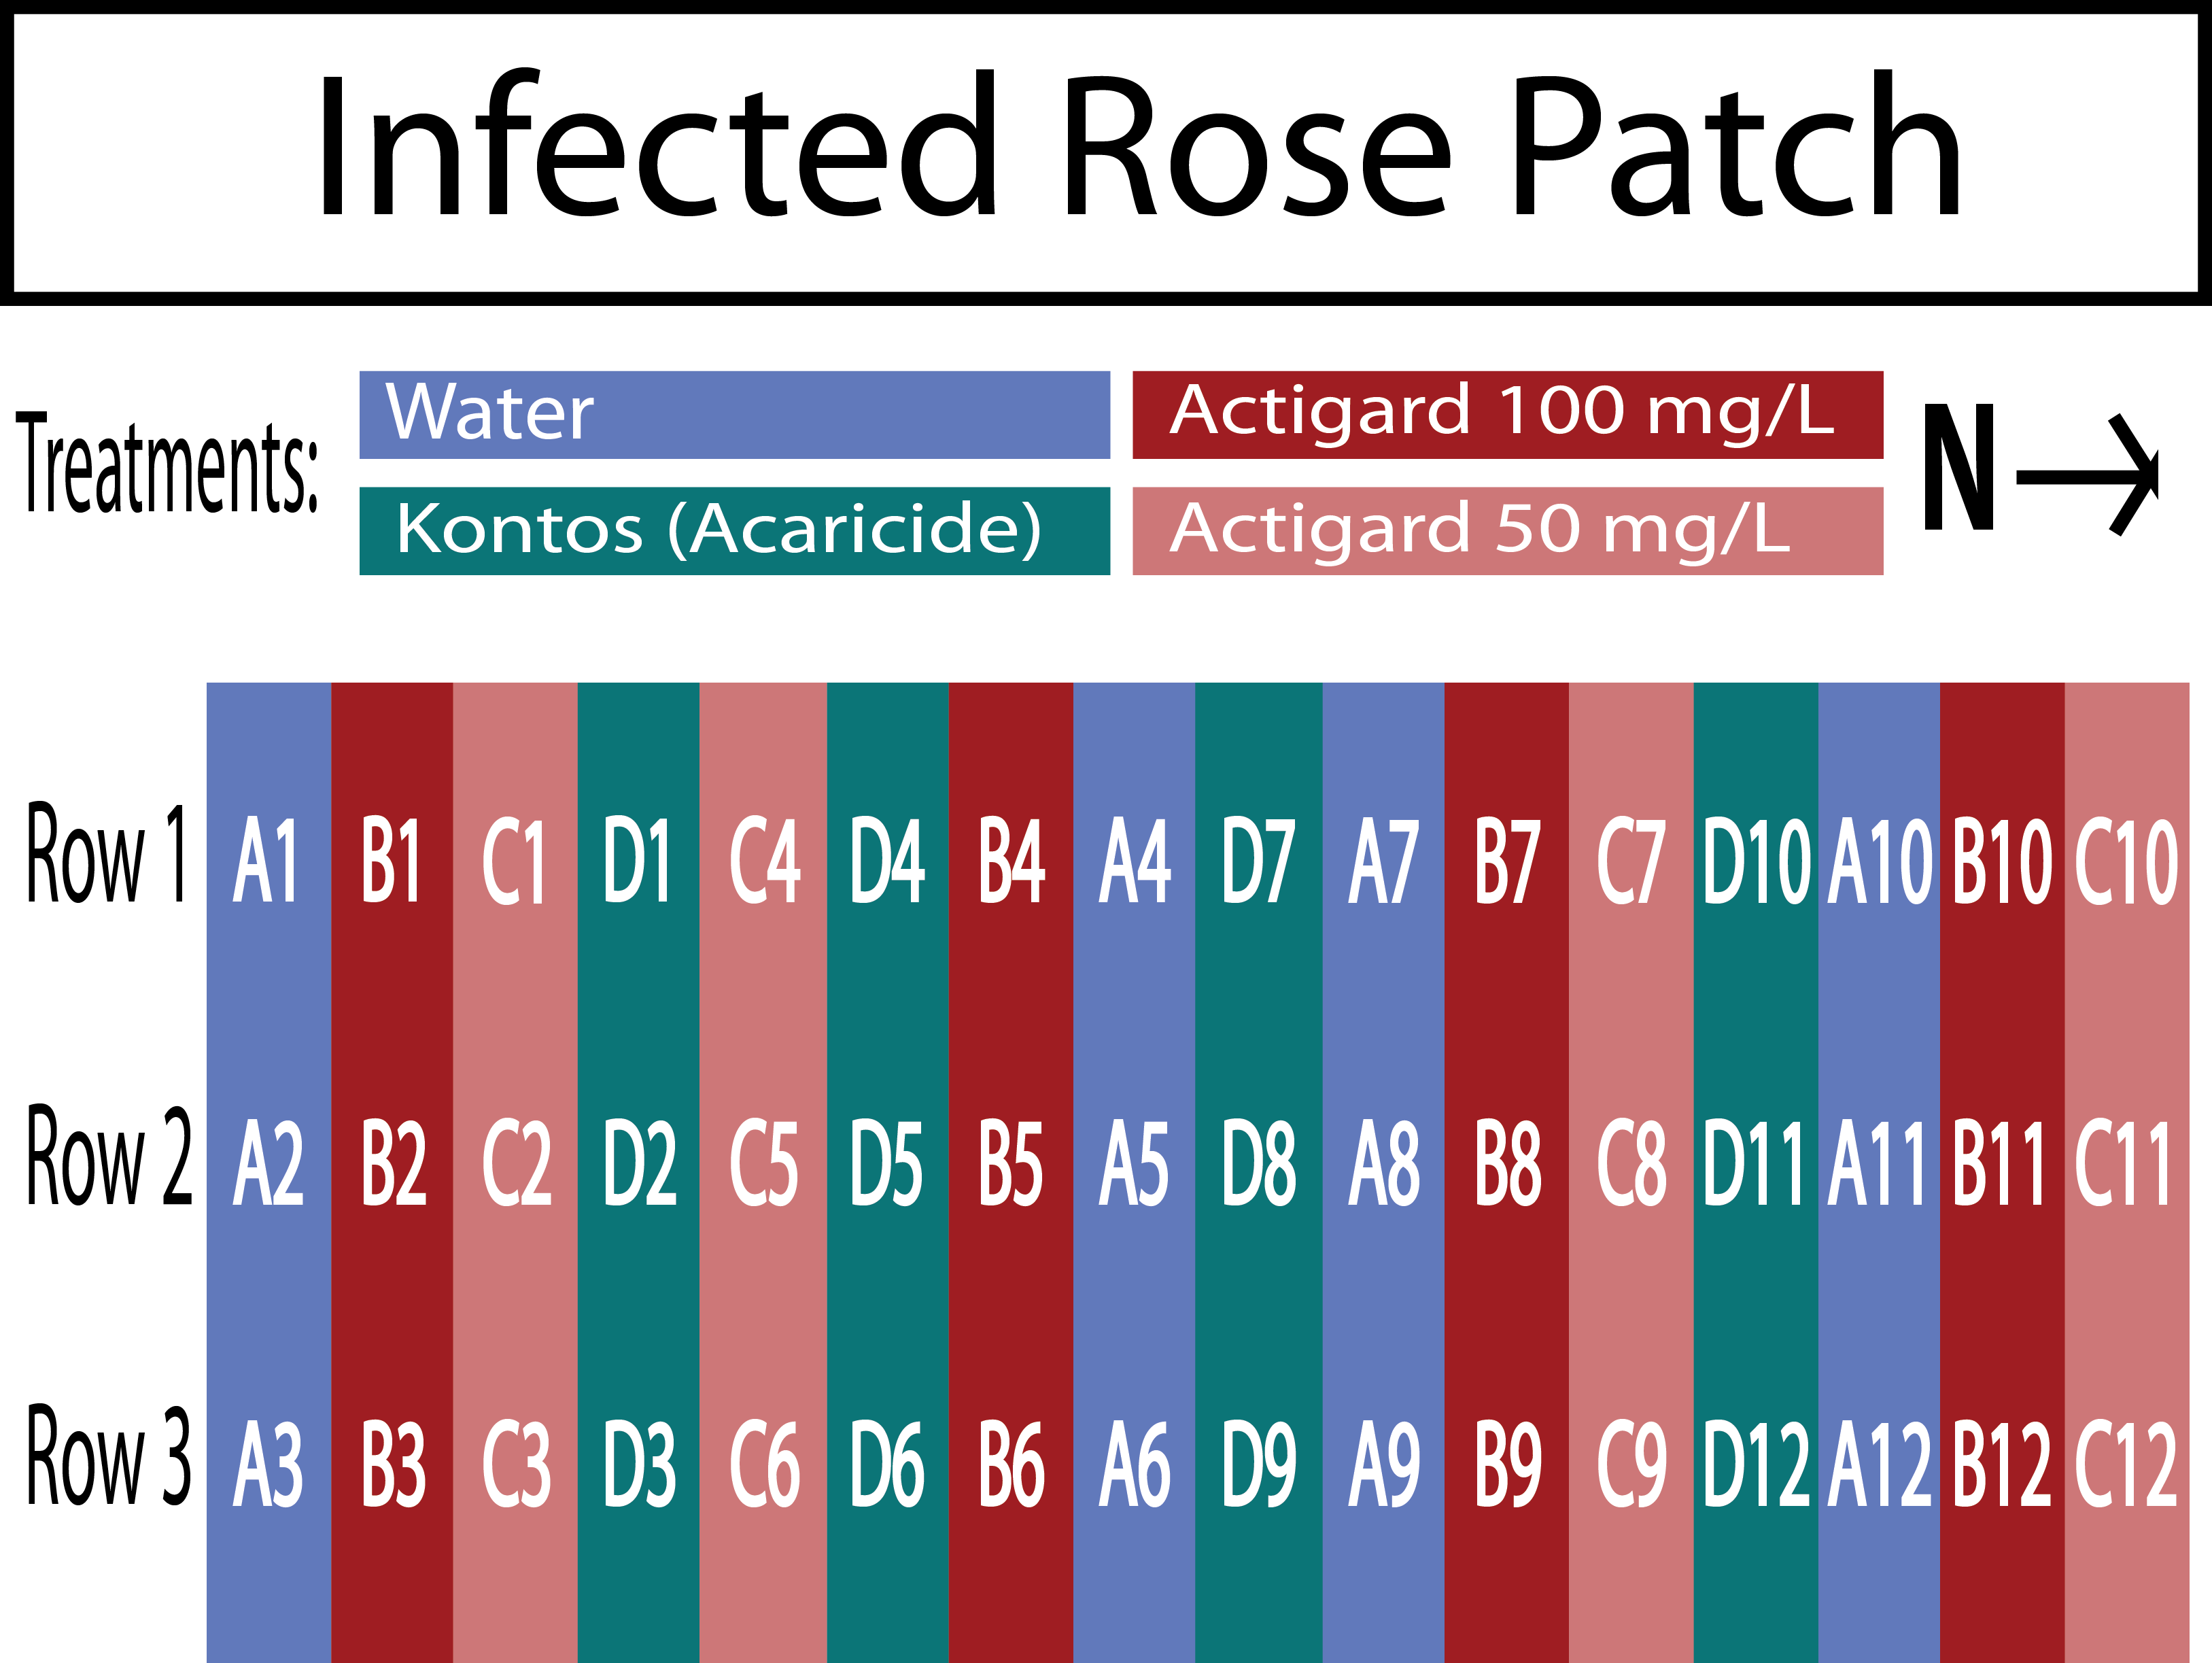
\includegraphics[width=0.8\linewidth]{figure/rrv_asm_plot_2018_griffin} \end{center}

  Figure 10: Field design for testing the potential of Acibenzolar-S-Methyl to reduce populations of \emph{P. fructiphilus} by inducing Systemic Acquired Resistance in Pink Double Knock Out® roses. Trials were conducted for three months from August to October 2018 in Griffin, GA. Four treatments were applied weekly for 12 weeks: Blue = Water Red = Actigard50WG 100 mg/L (High rate), Pink = Actigard50WG 100 mg/L (Half rate) Turquoise = Kontos (Label rate). Flower cuttings were be taken weekly to record \emph{P. fructiphilus} numbers.

  \textbf{Plot Design - 2019}
  \begin{center}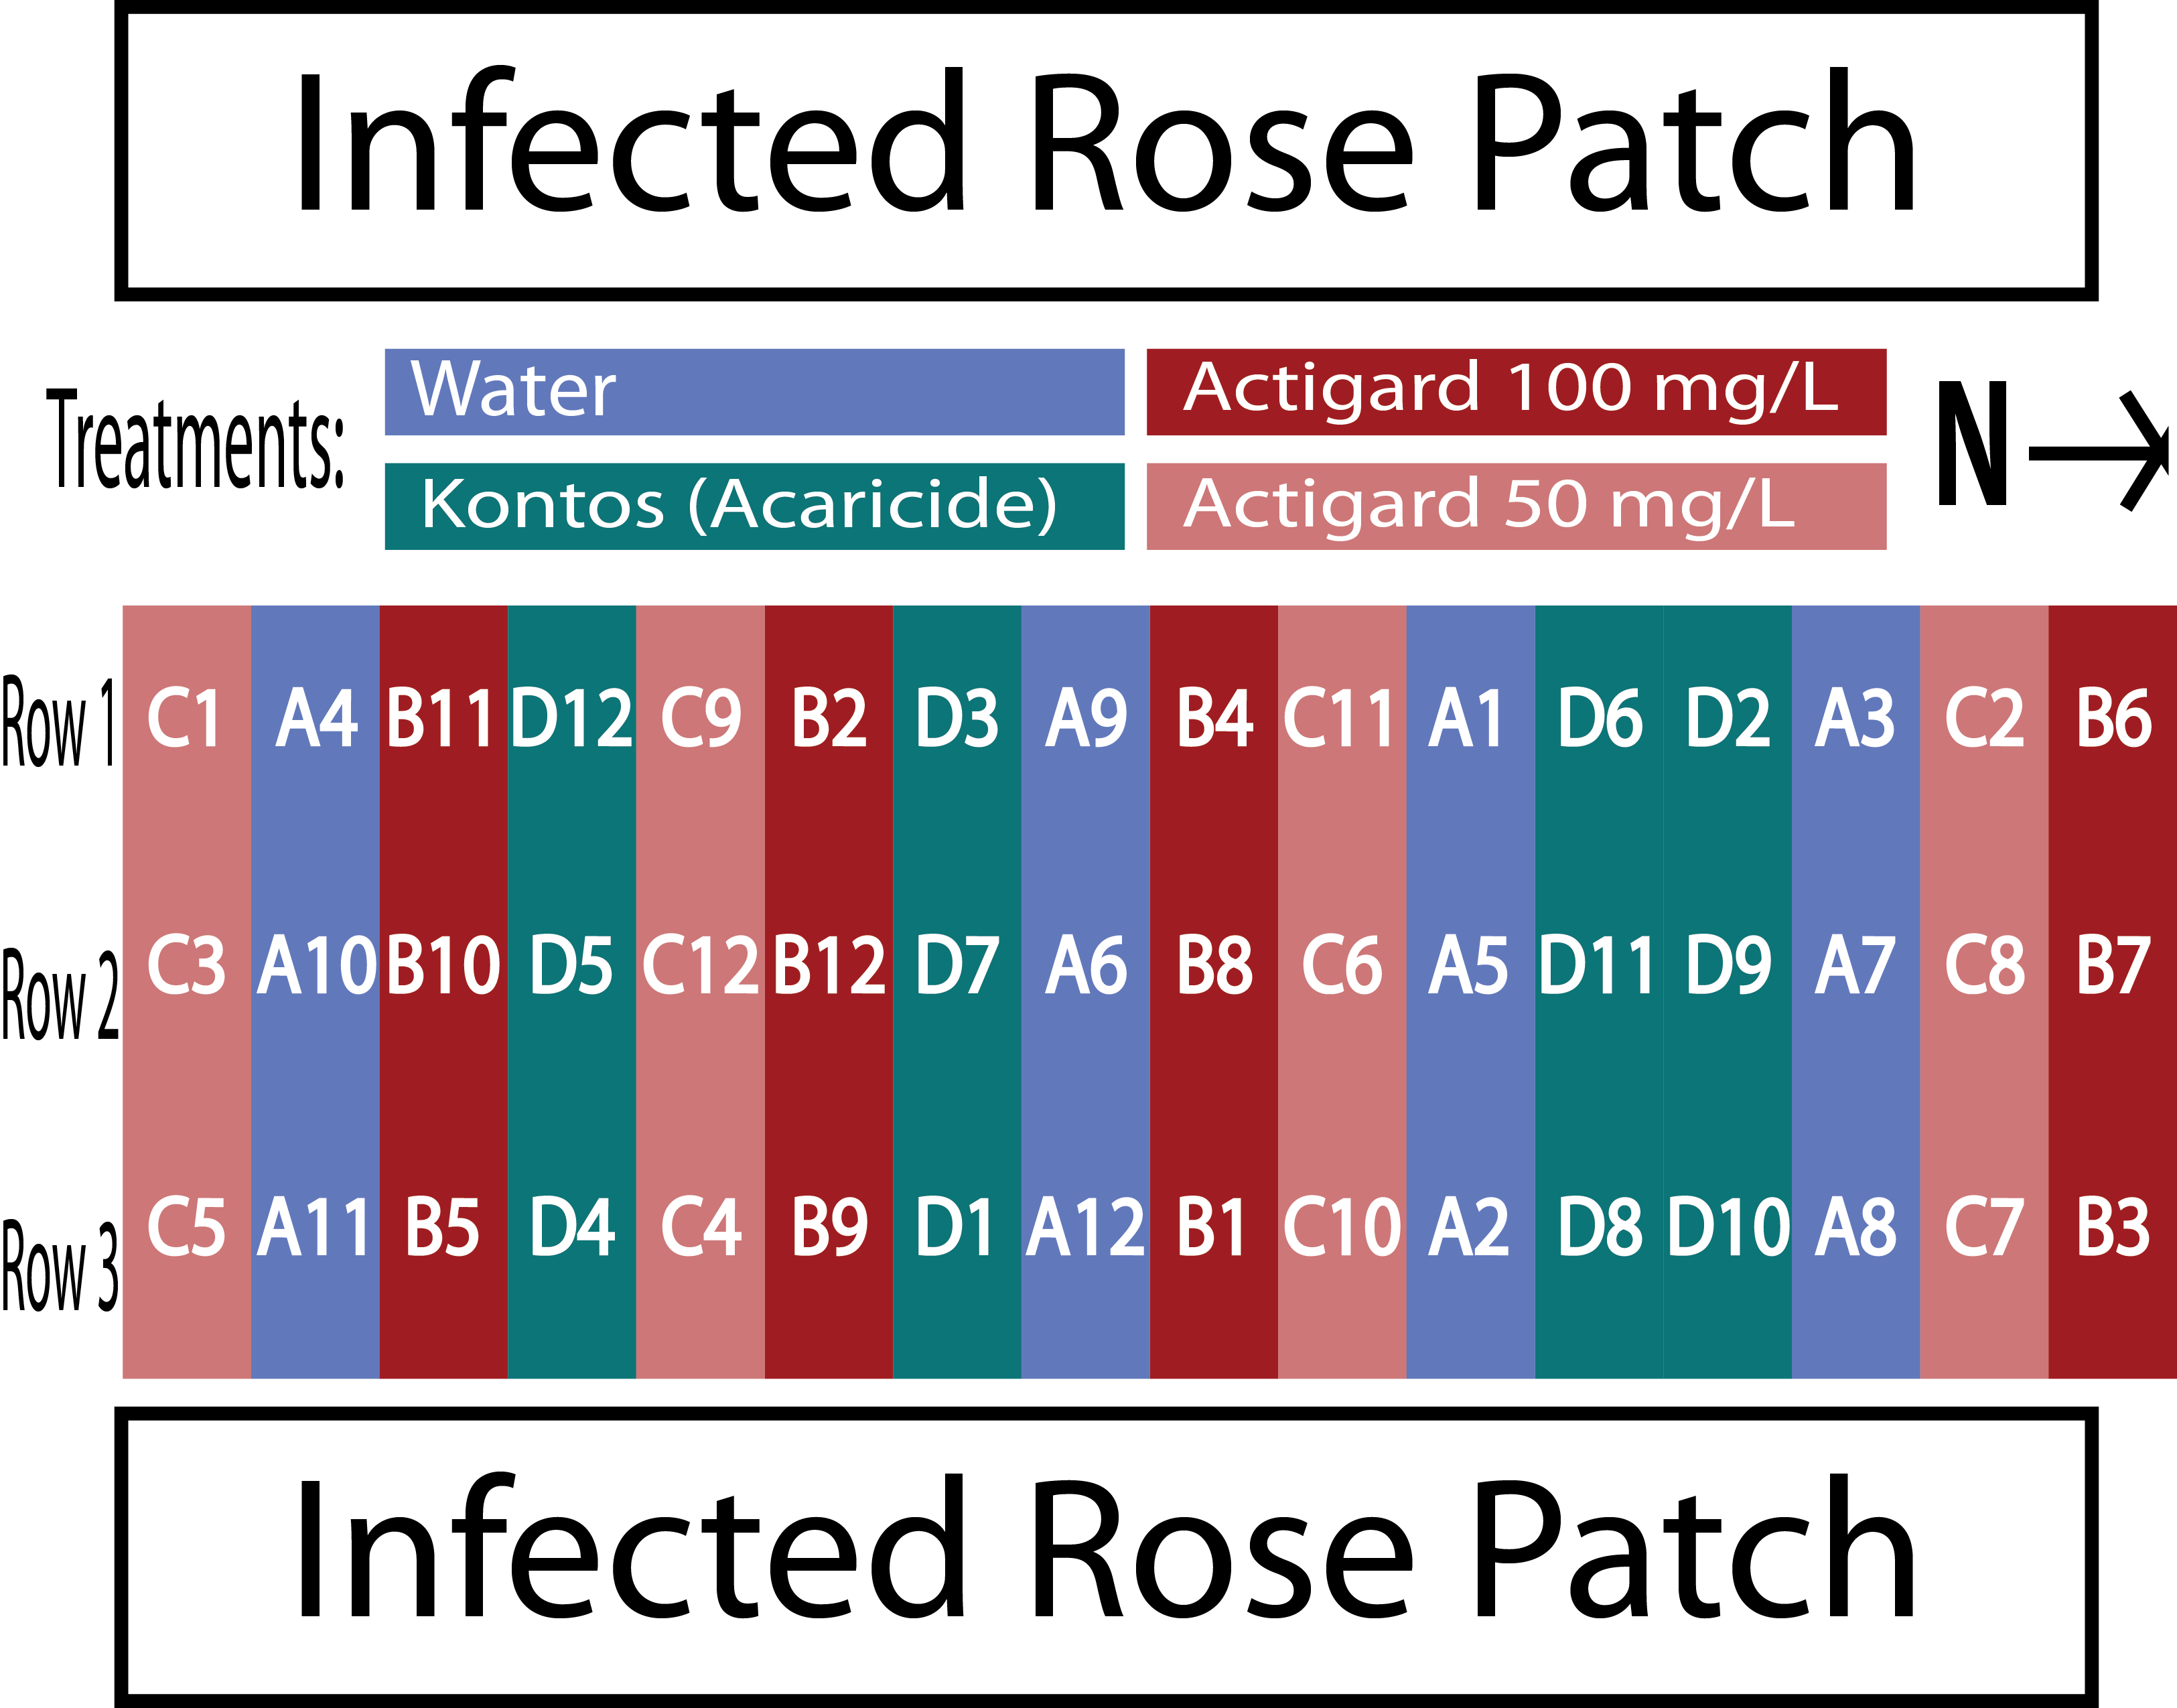
\includegraphics[width=0.8\linewidth]{figure/rrv_asm_plot_2019_griffin} \end{center}

  Figure 11: Field design for testing the potential of Acibenzolar-S-Methyl to reduce populations of \emph{P. fructiphilus} by inducing Systemic Acquired Resistance in Pink Double Knock Out® roses. Trials were conducted for three months from September to December 2019 in Griffin, GA. Four treatments were applied weekly fo 12 weeks: Blue = Water Red = Actigard50WG 100 mg/L (High rate), Pink = Actigard50WG 100 mg/L (Half rate) Turquoise = Kontos (Label rate). Flower cuttings were be taken weekly to record \emph{P. fructiphilus} numbers.

  \hypertarget{ipm-trials}{%
  \section{\texorpdfstring{4.2 Integrating Pest Management Methods to control \emph{Phyllocoptes fructiphilus}}{4.2 Integrating Pest Management Methods to control Phyllocoptes fructiphilus}}\label{ipm-trials}}

  \hypertarget{problem-statement-3}{%
  \subsubsection{4.2.1 Problem Statement}\label{problem-statement-3}}

  \hypertarget{proposal-we-propose-testing-various-pest-management-treatments-including-predatory-mites-to-reduce-populations-of-phyllocoptes-fructiphilus}{%
  \subsubsection{\texorpdfstring{4.2.2 Proposal: We propose testing various pest management treatments including predatory mites to reduce populations of \emph{Phyllocoptes fructiphilus}}{4.2.2 Proposal: We propose testing various pest management treatments including predatory mites to reduce populations of Phyllocoptes fructiphilus}}\label{proposal-we-propose-testing-various-pest-management-treatments-including-predatory-mites-to-reduce-populations-of-phyllocoptes-fructiphilus}}

  We propose testing two different SAR-inducers as well as predatory mites for their ability to reduce populations of \emph{P. fructiphilus}. We also intend to combine the effects of predatory mites with a SAR-inducer to determine if these treatments are compatible. All testing will be done in areas with high pest pressure in Georgia. Our hypothesis is that there will be fewer \emph{P. fructiphilus} on plants treated with the SAR-inducers when compared to the water treated control group, and even fewer mites found on plants treated with the combination of a SAR-inducer and predatory mites.

  \hypertarget{materials-methods-4}{%
  \subsubsection{4.2.3 Materials \& Methods}\label{materials-methods-4}}

  Our studies are designed to investigate if predatory phytoseiid mites such as \emph{A. swirskii} can be combined with roses' natural systemic activated resistance (SAR) to manage populations of the plant-parasitic mite, \emph{P. fructiphilus}, the vector of Rose Rosette Virus (RRV). Our findings will be used to develop Integrated Pest Management (IPM) programs for \emph{P. fructiphilus} management.

  \textbf{Roses}
  This will be a 12-week experiment conducted from August to October simultaneously in Griffin, GA and Athens, GA.
  The Athens site will be given 96 Pink Double Knock Out® Roses (Star Roses and Plants, West Grove, PA, USA), while Griffin will use 54 roses due to the smaller plot area available. Bare root roses will be planted 2 months before the trials begin to allow new flush to form. Rose planting media and environmental conditions will be the same as previously described.

  \textbf{Mite Infestation}
  \emph{Phyllocoptes fructiphilus} are present in the landscape of Georgia. Rose cuttings \textasciitilde10 cm will be taken from roses showing symptoms of Rose Rosette Disease in the landscape and placed in each rose pot on the 1st, 5th and 9th week of the experiment.

  \textbf{Predatory mites}

  \emph{Amblyseius swirskii} mites will be applied on the 1st, 5th and 9th week of the experiment. These mites are deployed from polyethylene fiber sachets containing live colonies of \emph{A. swirskii} and a mite which they consume for food. There is a small hole at the bottom of these sachets which allows the mites to be slowly released into the environment.

  \textbf{Field Treatments}
  \begin{enumerate}
  \def\labelenumi{\arabic{enumi}.}
  \tightlist
  \item
    Water - Control
  \item
    Actigard - 100 mg/L
  \item
    Ninja - label rate
  \item
    Kontos - label rate
  \item
    \emph{A. swirskii} (one sachet per rose treated)
  \item
    \emph{A. swirskii} + Ninja (one sachet per rose treated, label rate)
  \end{enumerate}
  \textbf{Data Collection}

  Georgia collaborators will be collecting flower samples from all roses once before beginning the treatments on week 1 and once at the end of the experiment on week 12. For weeks 2 through 11, Georgia collaborators will collect flower samples starting from the top rows of each block every week, until each row has been sampled three times (see \emph{Figure 12} and \emph{Figure 13}). Georgia collaborators rate disease severity for each rose every week before they spray, rating roses according to the Horsfall-Barratt Scale (Horsfall 1945). Roses displaying symptoms of RRD will have tissues sent to the Plant Disease Diagnostic Clinic at the North Florida Reasearch and Extension Center(PDC) for virus confirmation.

  \textbf{Sample Processing}
  \begin{itemize}
  \tightlist
  \item
    A flower cutting of about \textasciitilde12 cm will be take and placed the flower petal side down into 50 ml centrifuge tubes filled with 15 ml of 95\% ethanol so the entire flower is submerged over the sepals. Once the lid is is secure, the the tube will be shaken vigorously for a few seconds to help dislodge any mites. Samples will be processed using the washing methods of Monfreda et al. (2007), eriophyoid mites will be counted and identified as previously described.
  \end{itemize}
  \textbf{Plot Design - Athens}

  The site at Athens, GA has space for five blocks: A, B, C, D and E. Each block is a 3 \(\times\) 6 plot with 18 plants, with three plants in each treatment. The experiments will be run for 12 weeks. We will be sampling flower cuttings from two rows each week, starting with the top rows (1-15 and 16-30 for week one) of each block and rotating to the next row each week (31-45 and 46-60 on week 2) continuing until all rows have been sampled three times. In order to avoid confusion, each rose pot will be labeled with a stake that has the plant number and treatment abbreviation: (W, A, K, M, N, +) written on it. Applications will be done on the same day each week, weather permitting, preferably at the beginning of the week.
  \begin{center}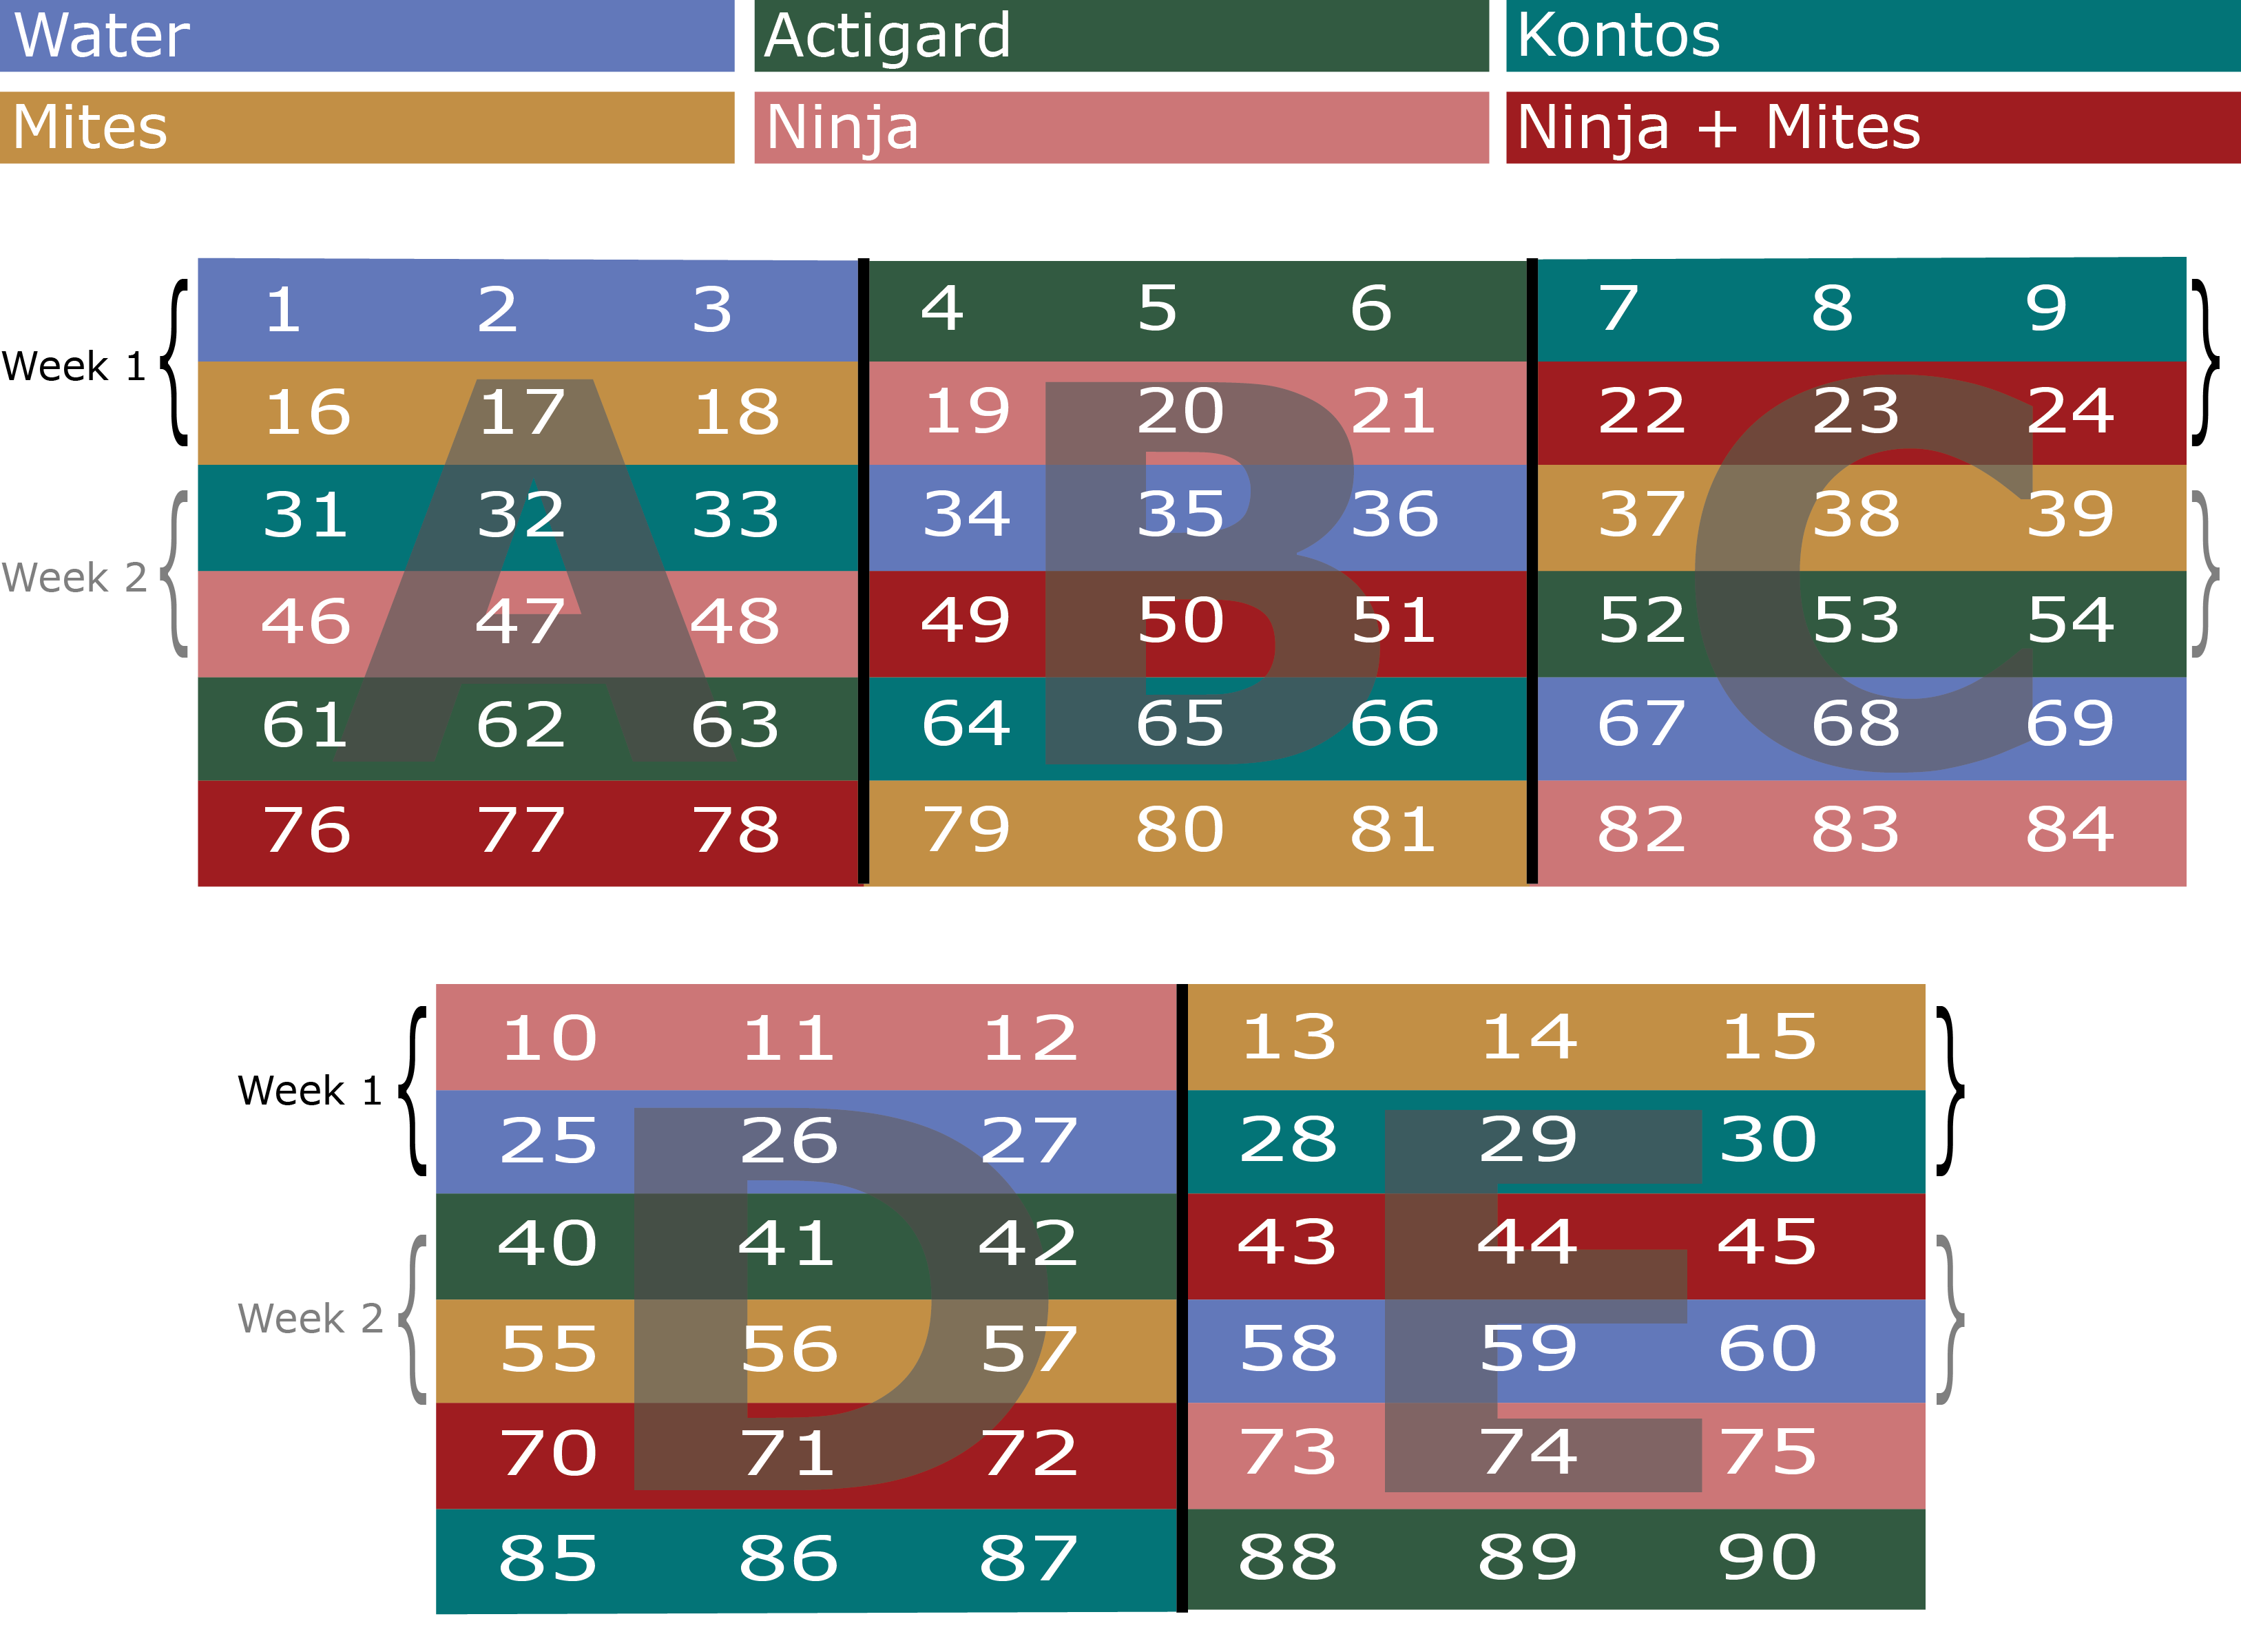
\includegraphics[width=0.8\linewidth]{figure/rrv_ipm_plot_map_2019_athens} \end{center}

  Figure 12: Field design for Integrated Pest Management trials on Pink Double Knock Out® roses to control \emph{P. fructiphilus} in Athens, GA with five treatments. W = Water A = Actigard50WG, K = Kontos, M = \emph{A. swirkii} predatory mite sachets, N = SP2700 (Trade name: Ninja, SePro), + = \emph{A. swirskii} + Ninja combined treatments. All products were applied at their label rates for 12 weeks. Flower cuttings were taken weekly to record \emph{P. fructiphilus} numbers.

  \textbf{Plot Design - Griffin}

  The site at Griffin, GA has space for three blocks: X, Y, and Z. Each block is a 3 \(\times\) 6 plot with 18 plants, with three plants in each treatment. This experiment was run for 12 weeks as well. We will be sampling flower cuttings from two rows each week, starting with the top rows (1-9 and 10-18 for week one) of each block and rotating to the next row each week (19-27 and 28-36 on week 2) continuing until all rows have been sampled three times. Labels and applications were conducted in the same manner as previously described.
  \begin{center}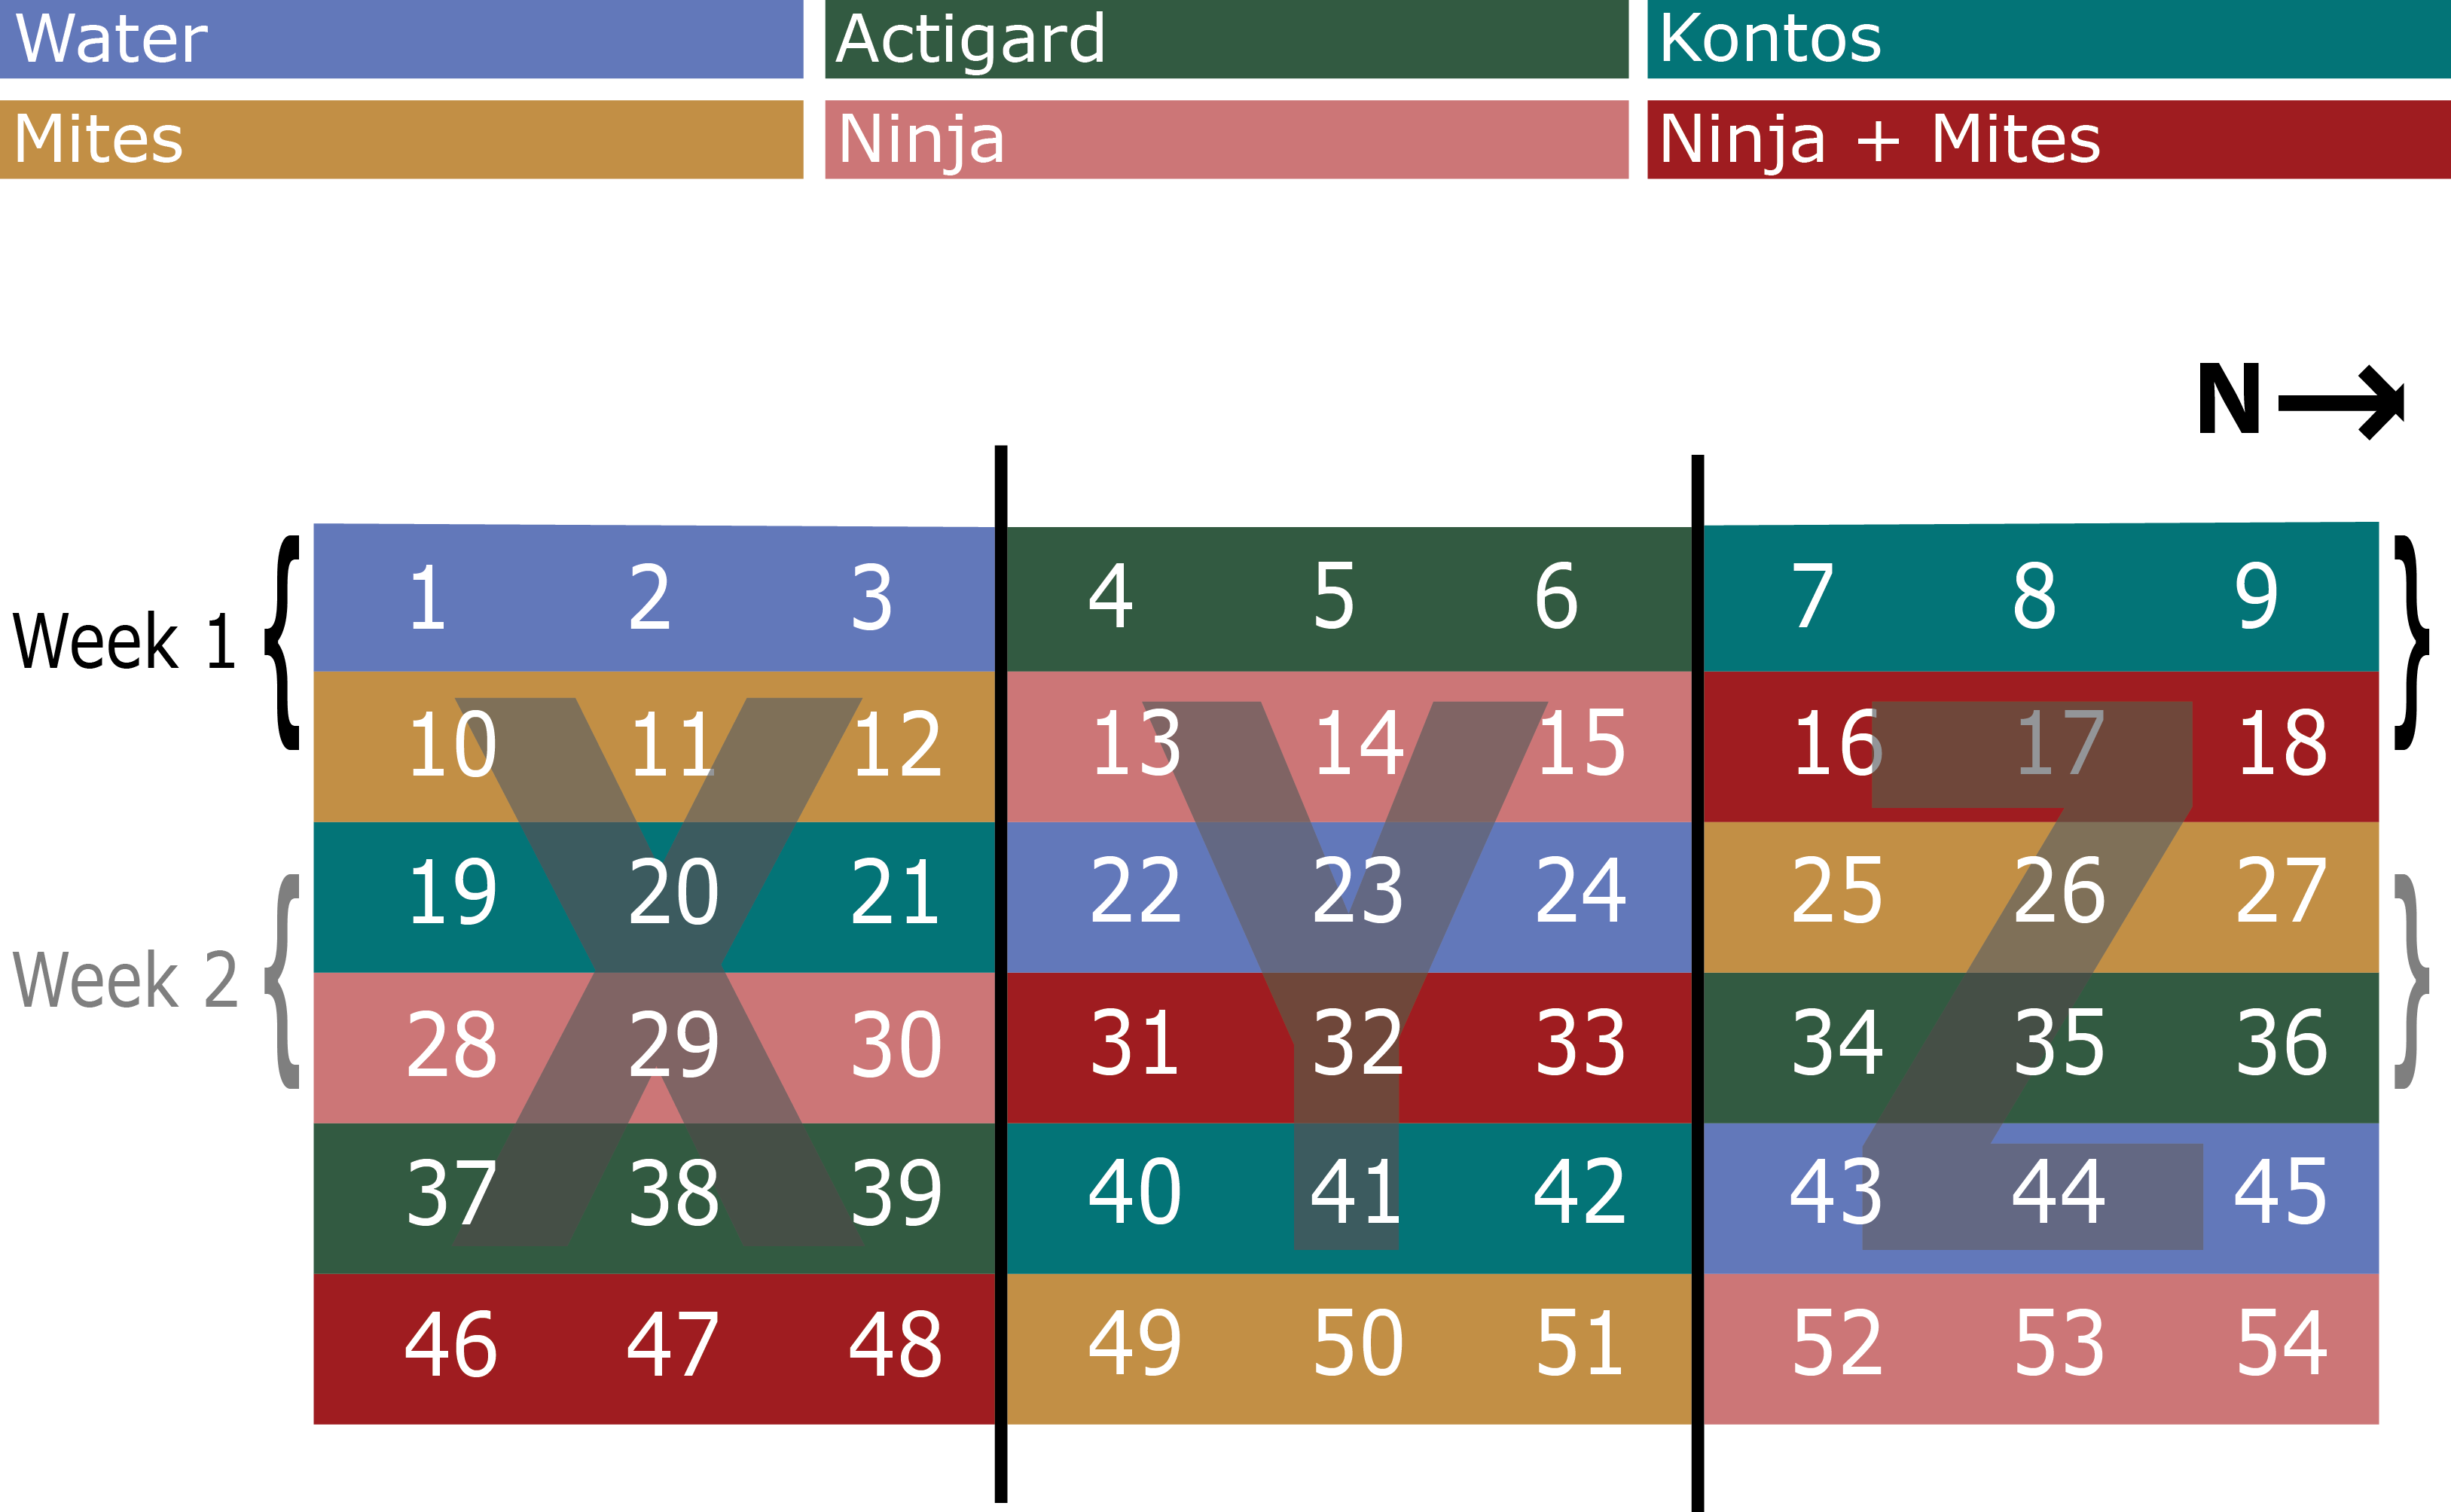
\includegraphics[width=0.8\linewidth]{figure/rrv_ipm_plot_map_2019_griffin} \end{center}

  Figure 13: Field design for Integrated Pest Management trials on Pink Double Knock Out® roses to control \emph{P. fructiphilus} in Griffin, GA with five treatments. W = Water A = Actigard50WG, K = Kontos, M = \emph{A. swirkii} predatory mite sachets, N = SP2700 (Trade name: Ninja, SePro), + = \emph{A. swirskii} + Ninja combined treatments. All products were applied at their label rates for 12 weeks. Flower cuttings were taken weekly to record \emph{P. fructiphilus} numbers.
  \begin{center}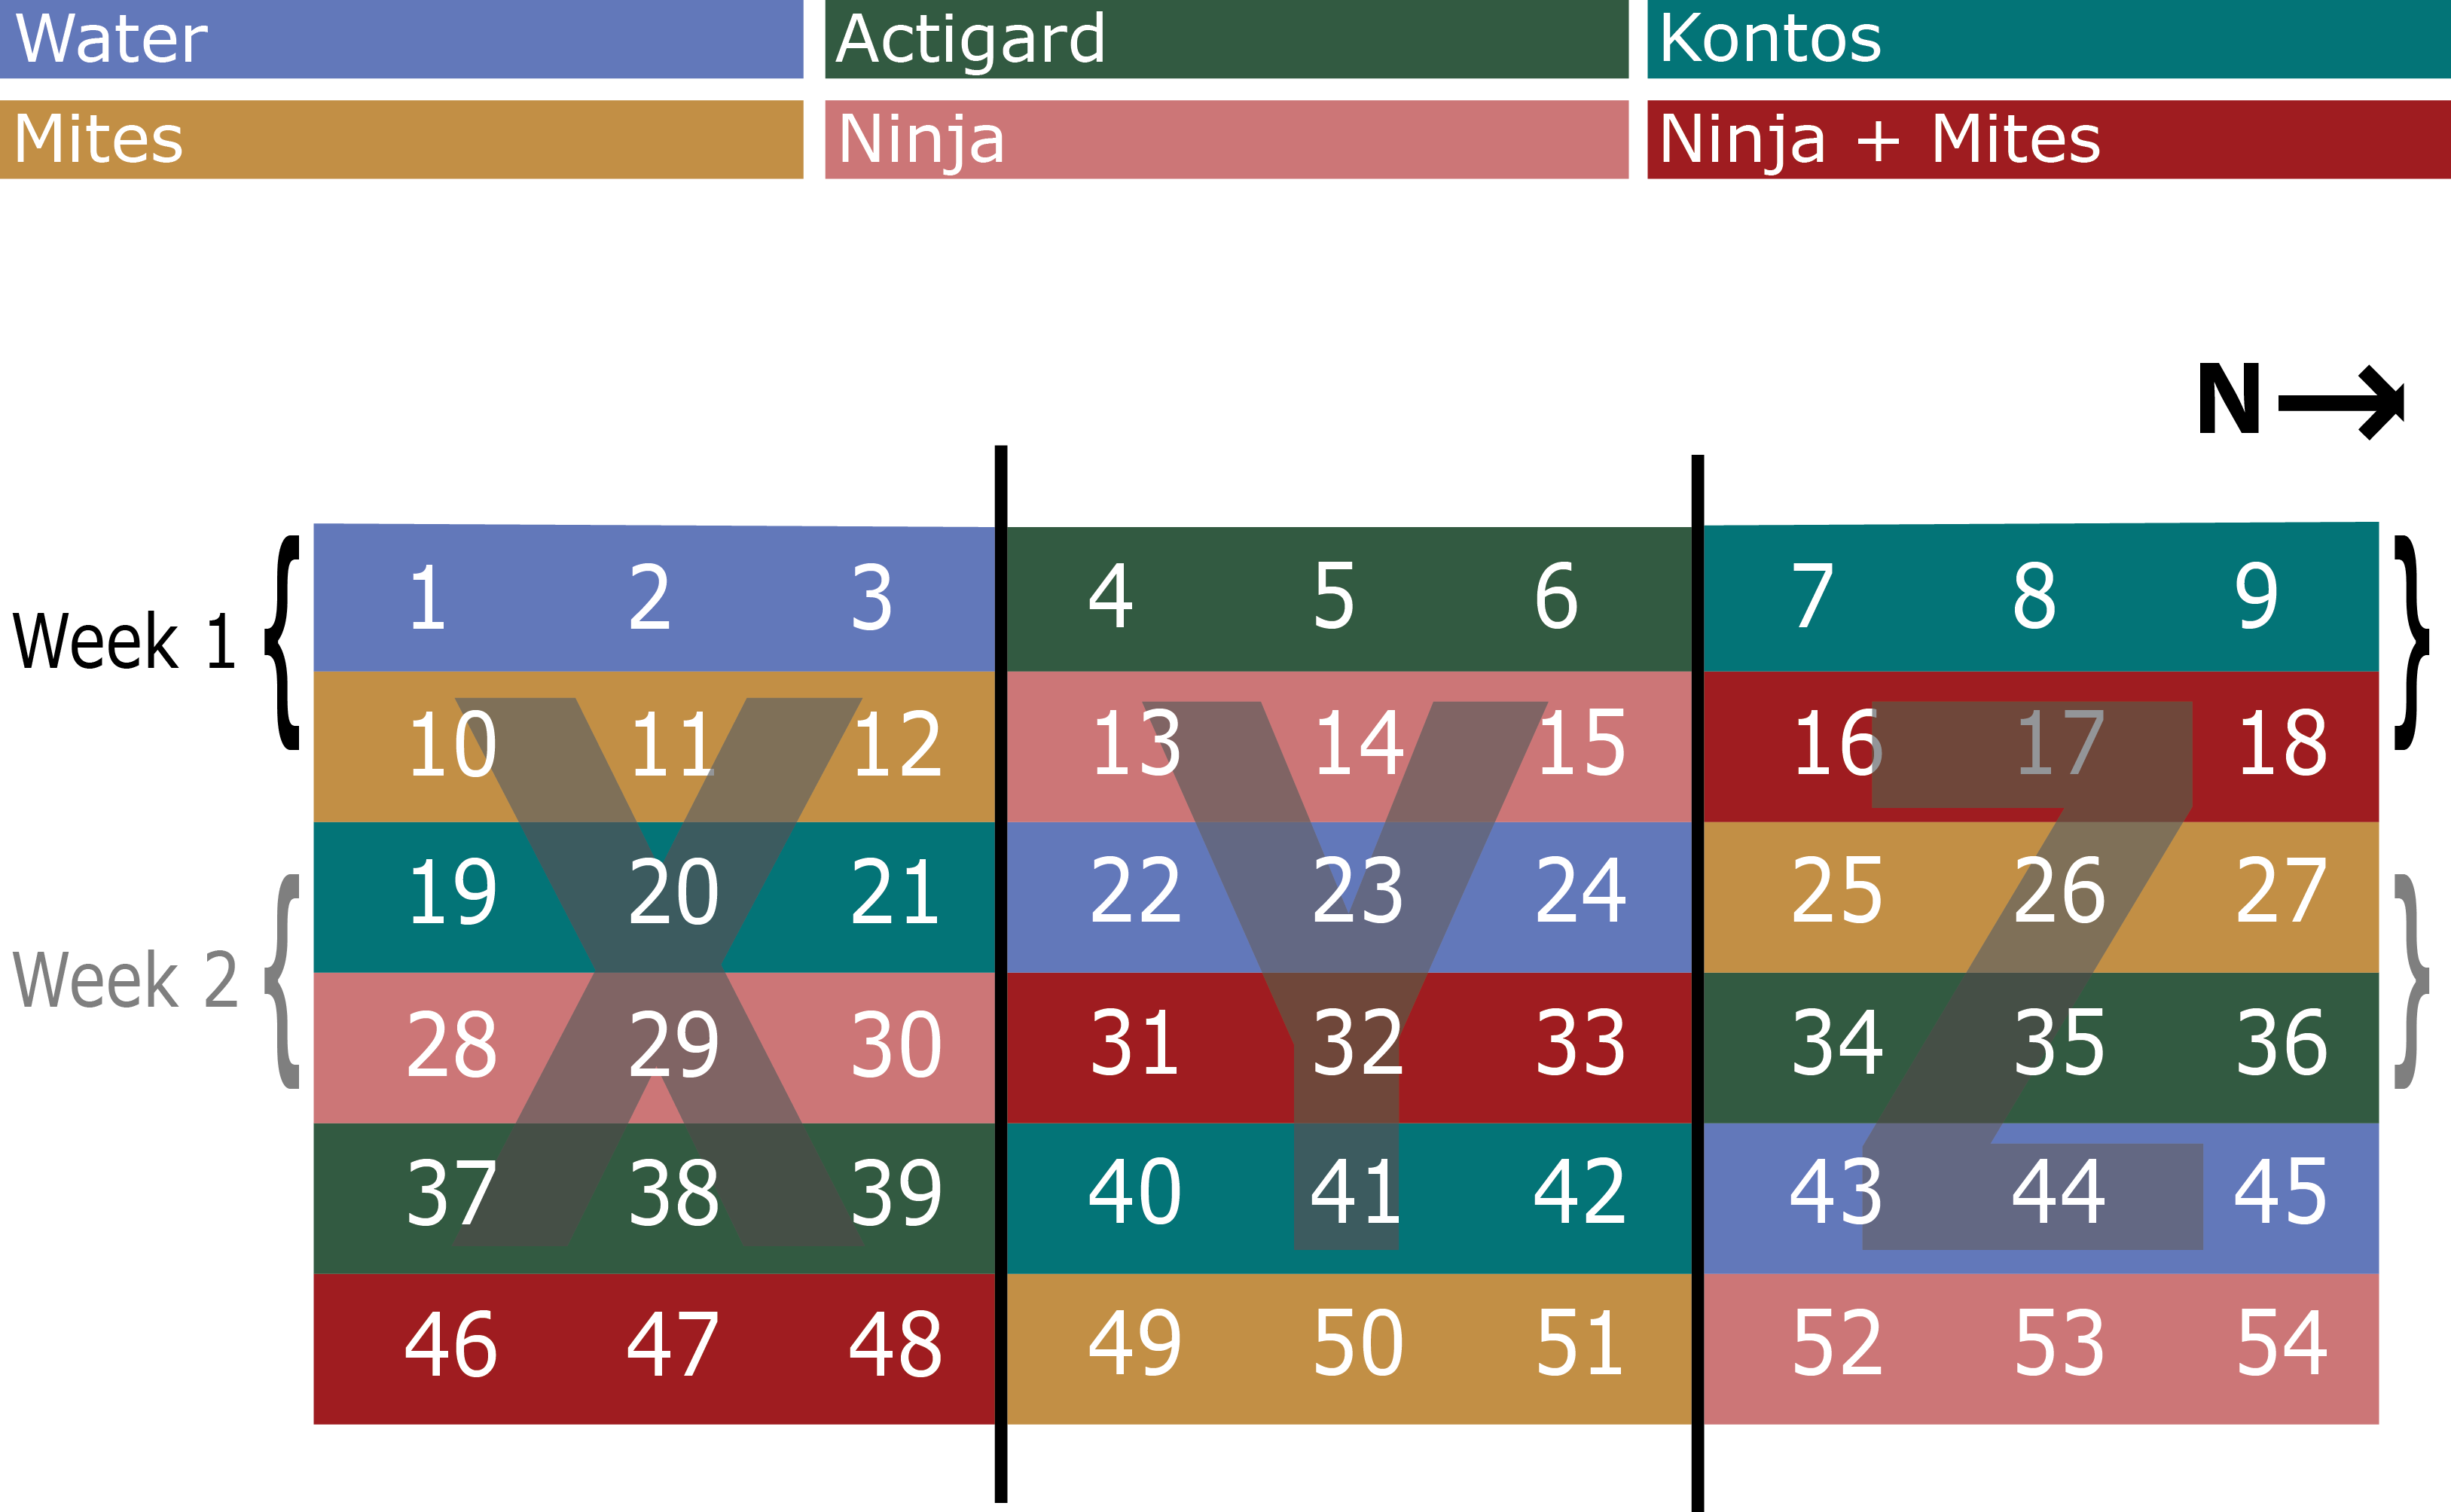
\includegraphics[width=0.8\linewidth]{figure/rrv_ipm_plot_map_2019_griffin} \end{center}

  Figure 14: Field design for Integrated Pest Management trials on Pink Double Knock Out® roses to control \emph{P. fructiphilus} in Tallahassee, FL with five treatments: Water, Actigard50WG, Kontos, \emph{Amblyseius swirkii} predatory mite sachets, and \emph{A. swirskii} + Actigard combined treatments. All products were applied at their label rates for 12 weeks. Flower cuttings were taken weekly to record \emph{P. fructiphilus} numbers.

  
\includegraphics[width=3.47in]{figure/reed}

  Figure 15: Number of \emph{Phyllocoptes fructiphilus} found in rose samples with five treatments. Statistical significance was determined using Tukey contrasts for multiple Comparisons of means. Groups which share letters are not statistically different from one another. a = 0.05

  \hypertarget{first-report-of-the-brevipalpus-transmitted-trombidiformes-tenuipalpidae-orchid-fleck-dichorhavirus-infecting-three-ornamentals-in-florida}{%
  \subsection{\texorpdfstring{First report of the \emph{Brevipalpus}-transmitted (Trombidiformes: Tenuipalpidae) \emph{Orchid fleck dichorhavirus} infecting three ornamentals in Florida}{First report of the Brevipalpus-transmitted (Trombidiformes: Tenuipalpidae) Orchid fleck dichorhavirus infecting three ornamentals in Florida}}\label{first-report-of-the-brevipalpus-transmitted-trombidiformes-tenuipalpidae-orchid-fleck-dichorhavirus-infecting-three-ornamentals-in-florida}}

  Austin \textbf{Fife}\textsuperscript{1}, Daniel \textbf{Carrillo}\textsuperscript{2}, Gary \textbf{Knox}\textsuperscript{3}, Fanny \textbf{Iriarte}\textsuperscript{4}, Kishore \textbf{Dey}\textsuperscript{5}, Avijit \textbf{Roy}\textsuperscript{6}, Ronald \textbf{Ochoa}\textsuperscript{7}, Gary \textbf{Bauchan}\textsuperscript{8}\(\dagger\), Mathews \textbf{Paret}\textsuperscript{4,9}, Xavier \textbf{Martini}\textsuperscript{1}*

  \textsuperscript{1} University of Florida, Department of Entomology and Nematology, North Florida Research and Education Center, Quincy FL 32351

  \textsuperscript{2} University of Florida, Department of Entomology and Nematology, Tropical Research and Education Center, Homestead FL 33031

  \textsuperscript{3} University of Florida, Department of Environmental Horticulture, North Florida Research and Education Center, Quincy FL 32351

  \textsuperscript{4} University of Florida, Department of Plant Pathology, North Florida Research and Education Center, Quincy FL 32351

  \textsuperscript{5} The Florida Department of Agriculture and Consumer Services, Division of Plant Industry, Section of Plant Pathology, Doyle Conner Building, 1911 SW 34th street, Gainesville, FL 32608

  \textsuperscript{6} United States Department of Agriculture -- Agriculture Research Service, Molecular Plant Pathology Laboratory, 10300 Baltimore Ave, Bldg. 4 BARC-West, Beltsville, MD 20705

  \textsuperscript{7} United States Department of Agriculture - Agriculture Research Service, Systematic Entomology Laboratory 10300 Baltimore Ave, Bldg. 5 BARC-West, Beltsville, MD 20705

  \textsuperscript{8} United States Department of Agriculture - Animal and Plant Health Inspection Service, Electron and Confocal Microscopy Unit, Bldg. 12 BARC-West, 10300 Baltimore Ave, Beltsville, MD 20705

  \textsuperscript{9} Plant Pathology Department, University of Florida, Gainesville, FL 32611

  *Corresponding author; E-mail: xmartini@ufl.edu Phone: 850-875-7160 Fax: 352-846-6617

  \pagebreak

  \hypertarget{abstract}{%
  \subsection{Abstract}\label{abstract}}

  We describe the first outbreaks of \emph{Orchid fleck dichorhavirus}, belonging to the orchid-infecting subgroup (OFV-Orc), from three unreported hosts: \emph{Liriope muscari}, cv. `Gigantea' (Decaisne) Bailey, \emph{Ophiopogon intermedius} Don and \emph{Aspidistra elatior} Blume (Asparagaceae: Nolinoidaea) in Leon and Alachua Counties, FL. Strains of OFV-Orc infect over 50 plant species belonging to the plant families Orchidaceae, Asparagaceae (Nolinoidaea), and infects \emph{Citrus} (Rutaceae) as citrus leprosis disease. The only known vectors of OFV-Orc are flat mites, genus \emph{Brevipalpus} (Trombidiformes: Tenuipalpidae). Florida has various plants in the landscape which \emph{Brevipalpus} spp. feed on, which are susceptible to infection by OFV-Orc.

  Chlorotic ringspots and flecking were seen affecting Liriopogons (\emph{Liriope} and \emph{Ophiopogon} spp.) in Leon County, FL. Nearby \emph{A. elatior} also appeared chlorotic. Local diagnostics returned negative for common plant pathogens, therefore new samples were sent to the Florida Department of Agriculture and Consumer Services (FDACS) and USDA-ARS for identification.

  Two orchid-infecting strains of Orchid fleck virus were detected via combinations of conventional RT-PCR, RT-qPCR, Sanger sequencing and High Throughput Sequencing. Amplicons shared 98\% nucleotide identity with OFV-Orc1 and OFV-Orc2 available in NCBI GenBank. Coinfections were seen in each county, but single strains of OFV-Orc were seen in \emph{L. muscari} (Alachua, OFV-Orc2) and \emph{A. elatior} (Leon, OFV-Orc1).

  Three potential mite vectors were identified via cryo-scanning electron microscopy (Cryo-SEM): \emph{Brevipalpus californicus} (Banks) sensu lato, \emph{B. obovatus} Donnadieu, and \emph{B. confusus} Baker.

  In conclusion, \emph{Orchid fleck dichorhavirus} is present in northern Florida, representing a risk for susceptible plants in the southeastern US.

  \hypertarget{keywords}{%
  \subsection{Keywords:}\label{keywords}}

  False spider mite, flat mite, \emph{Brevipalpus}-transmitted viruses, \emph{Liriope}, Nolinoidaea, \emph{Ophiopogon}, \emph{Aspidistra}, Ruscaceae, Rutaceae, Asparagaceae, orchid, Orchidaceae, pests, ornamental plants, Orchid fleck virus.

  \pagebreak

  \emph{Orchid fleck dichorhavirus}, commonly referred to as Orchid Fleck Virus (OFV), is the type member for the genus \emph{Dichorhavirus}, family \emph{Rhabdoviridae}. OFV is a bacilliform, nuclear rhabdovirus composed of two segments of single-stranded, negative-sense RNA which infects plants (Dietzgen et al. 2014, Walker et al. 2018, Amarasinghe et al. 2019). Flat mites from the genus \emph{Brevipalpus} (Trombidiformes: Tenuipalpidae) are the only group known to transmit dichorhaviruses (Maeda 1998), and \emph{Brevipalpus californicus} (Banks) \emph{sensu lato} are the only mites which do so in a persistent propagative manner (Kondo et al. 2003).

  OFV-infected plants exhibit various symptoms depending on the infected plant species as well as the strain of the OFV associated with the infection (Kubo et al. 2009a), but symptoms typically appear as chlorotic flecks, which ultimately coalesce into ringspot patterns.

  OFV was first described as infecting \emph{Cymbidium} orchids in Japan (Doi et al. 1977). OFV and OFV-like rhabdoviruses have been reported infecting orchids in Asia, Africa, North America, South America, Europe, and Oceania. The prevalence of OFV and its mite vector is thought to be associated with the movement of infected orchids (Dietzgen et al. 2018a).

  OFV naturally infects more than fifty species of Orchidaceae (Kitajima et al. 2010, Peng et al. 2013), some Asparagaceae (Nolinoidaea) (Mei et al. 2016, Dietzgen et al. 2018b), and Rutaceae, where it causes citrus leprosis-like symptoms (Roy et al. 2015, 2020, Cook et al. 2019, Olmedo-Velarde et al. 2021). Mechanical transmission of OFV is possible under laboratory conditions to some plants belonging to the plant families Chenopodiaceae, Aizoaceae, Fabaceae, and Solanaceae (Chang et al. 1976, Kondo et al. 2003, Peng et al. 2013).

  \hypertarget{virus-detection}{%
  \subsubsection{Virus Detection}\label{virus-detection}}

  During June 2020, chlorotic ringspot symptoms were observed on Giant Lilyturf \emph{Liriope} spp., cv. `Gigantea' in a landscape of Leon County, Florida (Figure 16). \emph{Liriope} belong to a group of plants in the family Asparagaceae, subfamily Nolinoidaea, comprised of grass-like monocotyledonous liliod plants native to southeastern Asia (Chase et al. 2009, Meng et al. 2021). \emph{Liriope} and the closely related \emph{Ophiopogon} (Asparagaceae: Nolinoidaea) are considered the most important ground cover plant in the southeastern United States (Mcharo et al. 2003).

  Viral infections of suspected leaf samples were initially tested at the Plant Disease Diagnostic Clinic at the North Florida Research and Education Center (NFREC) in Quincy, FL. All the samples were tested with one step conventional RT-PCR, and were found negative for begomovirus, carlavirus, potyvirus, tospovirus, \emph{Cucumber mosaic virus} and \emph{Tobacco mosaic virus}.

  As initial diagnostics were inconclusive, new samples were collected during July and August of 2020 to collect more of these putatively infected plants with ringspot symptoms. The plants collected included \emph{Liriope} spp. and \emph{Ophiopogon} spp., as well as \emph{Aspidistra elatior} Blume (Asparagaceae: Nolinoidaea). \emph{A. elatior} was suspected to be infected, due to both its proximity to infected \emph{Liriope} and the presence of unusually chlorotic leaves (Figure 17). Upon collection, the new samples were sent to the Florida Department of Agriculture and Consumer Services (FDACS) for identification.

  The FDACS determined eventually that the pathogen was \emph{Orchid fleck dichorhavirus} using previously published primers and methods to conduct RT-PCR and Sanger sequencing (Kubo et al. 2006b, 2006a, 2009a, Kubo et al. 2009b, Ramos-González et al. 2015). Orchid subgroup 1, OFV-Orc was identified following the methods described in Kondo et al. (2017). Sequencing demonstrated a shared 98\% nucleotide identity with the orchid strain subgroup, OFV-Orc (isolates So and Br with GenBank Accession numbers: AB244418 and MK522807, respectively) (Kondo et al. 2006, 2017).

  These samples from FDACS were subsequently retested by the USDA-ARS, in conjunction with tests of fresh samples from both Alachua and Leon counties. The USDA used RT-PCR, RT-qPCR, and High Throughput Sequencing (HTS) in sequence to reconfirm the presence of \emph{Orchid fleck dichorhavirus}. RT-PCR and qPCR with Generic R2-Dicho-GF and R2-Dicho-GR primers amplifed \textasciitilde800 nt of L-gene (RNA2) amplicon (Roy et al. 2020), and OFV-Orc1 and OFV-Orc2 were detected in both \emph{O. intermedius} and \emph{A. elatior} from Leon County.

  HTS reaffirmed the presence of OFV-Orc1 and OFV-Orc2 strains in Leon and Alachua counties (Table 1). HTS results from Leon County revealed that \emph{L. muscari} were coinfected with both strains (OFV-Orc1 and OFV-Orc2), while \emph{A. elatior} were solely infected with OFV-Orc1. HTS of \emph{L. muscari} from Alachua County revealed infections with the OFV-Orc2 strain.

  After the initial identification by FDACS of OFV-Orc strains, mite samples were collected from symptomatic Asparagaceae in Leon County. Most mites collected were Tenuipalpid mites (flat mites or false spider mites), a known pest of ornamental plants, some of which are known to act as vectors for plant viruses (Childers et al. 2003, Childers and Rodrigues 2011).

  \hypertarget{mite-description}{%
  \subsubsection{Mite Description}\label{mite-description}}

  Mite taxonomy is complicated by cryptic species complexes which occur in many plant-feeding groups of the Acari (Umina and Hoffmann 1999, Skoracka and Dabert 2010, Arthur et al. 2011, Skoracka et al. 2013), including tenuipalpid mites from the genus \emph{Brevipalpus} (Navia et al. 2013). The commonly used phase-contrast microscopy is insufficient to detect some diagnostic characters for separation of cryptic species, instead best practices recommend the combination of Differential Interference Contrast (DIC) Microscopy and Scanning Electron Microscopy along with molecular methods to separate cryptic species (Beard et al. 2015).

  The flat mites collected were initially suspected to belong to \emph{B. californicus} after inspection with phase contrast microscopy. Subsequent observation via DIC microscopy at FDACS agreed with this tentative identification. Unfortunately, the \emph{B. californicus} s.l. species group, \emph{sensu} Baker and Tuttle (1987) is suspected to contain cryptic species (Childers and Rodrigues 2011, Rodrigues and Childers 2013). New mite samples were collected from symptomatic liriopogons and \emph{A. elatior} in Leon County and sent to USDA-ARS's Electron and Confocal Microscopy Unit for analysis. Three mite species were recovered and examined under cryo-scanning electron microscopy (Cryo-SEM): \emph{B. californicus} s.l. (Figure 18), \emph{B. obovatus} Donnadieu and \emph{B. confusus} Baker (Figure 19).

  The first report of OFV in the US is thought to be Ko et al. (1985), who describes nuclear inclusions caused by an undescribed bacilliform rhabdovirus in \emph{Brassia} orchids. The significance of this report is their description of the spoke-wheel configurations of the viral particles (Ko et al. 1985), a sign typically associated with OFV infection (Chang et al. 1976). Unfortunately, this article made no mention of mites or further investigations of the virus. The first report of OFV in the continental US was Bratsch et al. (2015), who confirmed the presence of OFV in \emph{Phalaenopsis} hybrids using Transmission Electron Microscopy of ultrathin sections of plant tissue as well as molecular sequence analysis. They also discuss the association of OFV with \emph{Brevipalpus} mites, but the authors did not make a conclusive species identification beyond suggesting that the mite vector belonged to the \emph{B. californicus} group, referring to Kondo et al. (2003)'s publication (Bratsch et al. 2015).

  Later reports of OFV described OFV infecting a previously undescribed Nolinoidaea hosts in Australia (Mei et al. 2016, Dietzgen et al. 2018b), including \emph{Liriope spicata} (Thunb.) Lour, a different species of liriopogon than those identified from the Florida sites. We are not aware of any reports of OFV infecting liriopogons, \emph{A. elatior} nor other Nolinoidaea in the US. Although Zheng et al. (2013) had mentioned an association between \emph{B. californicus} and \emph{A. elatior}, they never reported symptoms of OFV-Orc in this plant. We believe that our findings indicate the first report of OFV-Orc infecting ornamental Nolinoidaea in Florida, and possibly the US. This publication also marks the first reports of \emph{A. elatior} and \emph{Ophiopogon} spp. as natural hosts of OFV-Orc.

  OFV consists of two orchid strains (OFV-Orc1 and OFV-Orc2) and two citrus strains (OFV-Cit1 and OFV-Cit2) (Beltran-Beltran et al. 2020, Roy et al. 2020). The OFV strains detected in Florida are identical in gene order, content, and genome sequence to the orchid strains of OFV infecting citrus in Hawaii, Mexico, Colombia, and South Africa (Beltran-Beltran et al. 2020, Roy et al. 2020). Both OFV-Orc1 and OFV-Orc2 infect citrus (Roy et al. 2020), but none of the citrus strains have been reported from any orchid species. The \emph{Brevipalpus} mites collected from liriopogons and \emph{A. elatior} in Leon County were abundant on OFV-infected plants very near to citrus trees, some plants even surrounding the trunk. \emph{B. californicus} s. l. has been reported as a pest of citrus (Childers et al. 2003) and are often collected from citrus rinds (Baker 1949, Baker and Tuttle 1987). The proximity of these mite vectors to citrus raises the question: why these trees are not currently infected with OFV-Orc? It is important to note the uncertainty surrounding the vector for OFV-Orc. There are three mite species which have been recovered from OFV-Orc infected plants: \emph{B. californicus} s.l. (the most likely culprit), \emph{B. obovatus}, and \emph{B. confusus}. Each species has its own unique biology, and all have been implicated with a variety of different hosts. This suggests that the spread of OFV-Orc would be a function of various combinations of several potential factors, including host preferences, vectorial capacity, viral propagation/circulation in the vector, viral acquisition times, and feeding times required for transmission. Some of these factors have been tested: \emph{Brevipalpus} vectors have demonstrated such virus-vector specificity with \emph{Citrus leprosis virus N}--another dichorhavirus which causes citrus leprosis (Roy et al. 2013)--in studies done by Ferreira et al. (2020) and García-Escamilla et al. (2018). In these studies, \emph{Brevipalpus} mites were not able to transmit more than one virus. This could mean that the \emph{B. californicus} which we find on liriopogons and \emph{A. elatior} are not actually the same species as those found on citrus, or at least are not able to transmit OFV to citrus.

  Best practices for integrated pest management have not been created for controlling \emph{Brevipalpus} mites on these ornamentals, but methods designed to control \emph{Brevipalpus} in other systems may be applicable. The most common method used to control \emph{Bervipalpus} are synthetic acaricides (Andrade et al. 2010, 2019). Unfortunately, some acaricides and their residues can harm beneficial predatory mites as well (Fernández et al. 2017), even at low doses (Havasi et al. 2021), and mixing different chemistries can be detrimental for mite control (Vechia et al. 2018). In addition, pesticide resistance has been reported in various \emph{Brevipalpus} populations (Alves et al. 2000, Omoto et al. 2000, Campos and Omoto 2002, Rocha et al. 2021), due to exposure to pesticides used to control other arthropod pests (Vechia et al. 2021). In addition, predatory mites (Chen et al. 2006, Argolo et al. 2020), entomopathogenic fungi (Magalhães et al. 2005, Rossi-Zalaf et al. 2008, Peña et al. 2015, Revynthi et al. 2019) have shown promise for controlling other \emph{Brevipalpus} mites. Moreover, it is often possible to integrate different control techniques for improved management, such as combining predatory mites with compatible acaricides and entomopathogenic fungi (Reddy 2001, Midthassel et al. 2016, Andrade et al. 2019).

  In conclusion, detecting OFV in Florida represents a concern for horticulturists who grow orchids, \emph{Liriope}, \emph{Ophiopogon}, or other susceptible Asparagaceae species which are commonly used in landscaping. Florida is also home to a plethora of native and naturalized orchid species, many of which are threatened, including cultivated \emph{Vanilla} in southern Florida (Chambers et al. 2019) and the famous Ghost Orchid, {[}\emph{Dendrophylax lindenii} (Lindl.) Benth. ex Rolfe{]}. Citrus leprosis was present in Florida during the 1860's and almost eradicated by the mid-1960s (Knorr 1968, Knorr et al. 1968, Childers et al. 2003). An examination of herbarium specimens of Florida citrus found that this historical virus, Citrus leprosis dichorhavirus-N0, is distantly related to the modern strains of OFV (Kitajima et al. 2011, Hartung et al. 2015, Roy et al. 2020). The recent detection of OFV-Orc1 in South Africa (Cook et al. 2019) in \emph{C. sinensis} (Navel and Valencia orange) and OFV-Orc2 in Hawaii (Olmedo-Velarde et al. 2021) in \emph{C. reticulata} (mandarin) and \emph{C. jambhiri} (rough lemon) associated with leprosis-like symptoms highlights the threat of different strains of OFV on citrus, which will be a definite concern to the US multi-billion-dollar citrus industry already impacted by the Huanglongbing disease. \emph{B. californicus}, as well as \emph{B. yothersi}, are both known vectors of dichorhaviruses (OFV) (Kondo et al. 2003, García-Escamilla et al. 2018, Beltran-Beltran et al. 2020) and \emph{B. obovatus} is a suspected vector as well (Childers et al. 2003). All three mite species/complexes are present in Florida (Childers et al. 2003, Akyazi et al. 2017) (Figure 19), and are difficult to identify by non-experts, or without advanced methodologies. DNA barcoding (Armstrong and Ball 2005) or a similarly simple and accurate method for identification of these mite complexes is vital to determine which of these species are responsible for transmission of OFV-Orc, and therefore which mite populations need to be monitored or controlled. By doing so, we can determine the risk OFV-Orc represents for the native plants, agriculture and the ornamental/landscaping industries of Florida and the surrounding regions.

  \hypertarget{acknowledgements}{%
  \subsection{Acknowledgements}\label{acknowledgements}}

  We would like to give special thanks to the Tallahassee Museum for their patience, cooperation, and support with collecting plant samples. We also want to thank Drs. Sam Bolton, FDACS and Aline Tassi, Univ. of Sao Paulo, Brazil for checking the mites we have sent for species validation. Furthermore, we are grateful for Dr.~Marc S. Frank's identification of the Liriopogons collected. We are especially indebted to the late Dr.~Gary Bauchan for his contributions to this study and the field of acarology, he will be greatly missed. This research was partly funded by the USDA National Institute of Food and Agriculture, Hatch project FLA-NFC-005607. Mention of trade names or commercial products in this publication is solely for the purpose of providing specific information and does not imply recommendation or endorsement by the USDA; USDA is an equal opportunity provider and employer.

  \hypertarget{references}{%
  \subsection{References}\label{references}}

  \hypertarget{table-1-list-of-asparagaceae-nolinoidaea-species-with-verified-cases-of-orchid-fleck-dichorhavirus-collected-from-the-landscape-of-northern-florida}{%
  \subsection{\texorpdfstring{Table 1: List of Asparagaceae (Nolinoidaea) species with verified cases of \emph{Orchid fleck dichorhavirus}, collected from the landscape of northern Florida}{Table 1: List of Asparagaceae (Nolinoidaea) species with verified cases of Orchid fleck dichorhavirus, collected from the landscape of northern Florida}}\label{table-1-list-of-asparagaceae-nolinoidaea-species-with-verified-cases-of-orchid-fleck-dichorhavirus-collected-from-the-landscape-of-northern-florida}}
  \begin{longtable}[]{@{}
    >{\raggedright\arraybackslash}p{(\columnwidth - 6\tabcolsep) * \real{0.30}}
    >{\raggedright\arraybackslash}p{(\columnwidth - 6\tabcolsep) * \real{0.38}}
    >{\raggedright\arraybackslash}p{(\columnwidth - 6\tabcolsep) * \real{0.15}}
    >{\raggedright\arraybackslash}p{(\columnwidth - 6\tabcolsep) * \real{0.18}}@{}}
  \toprule
  Scientific Name & Common Names & County & Strains \\
  \midrule
  \endhead
  \emph{Liriope muscari} cv. `Gigantea'* (Decaisne) Bailey & Lilyturf, Orchardgrass, Monkeygrass & Alachua \& Leon & OFV-Orc1 \& OFV-Orc2 \\
  \emph{Ophiopogon intermedius}** Don & Aztec Grass, `Argenteomarginatus' & Leon & OFV-Orc1 \& OFV-Orc2 \\
  \emph{Aspidistra elatior} Blume & Cast Iron Plant, Bar-room Plant & Leon & OFV-Orc1 \& OFV-Orc2 \\
  \bottomrule
  \end{longtable}
  Table 1: * \emph{Liriope muscari} cv. `Gigantea' has been traditionally classified as \emph{L. gigantea} Hume by Broussard (2007) and Fantz et al. (2015), although this distinction has been challenged by Wang et al. (2014) and Masiero et al. (2020). * * \emph{O. intermedius} is sometimes misclassified as \emph{Liriope muscari} `Variegated Evergreen Giant' Fantz (2009) or `Grandiflora White' (Fantz 2009).

  \hypertarget{figure-captions}{%
  \subsection{Figure captions}\label{figure-captions}}

  Figure 16: Variety of symptoms expressed by \emph{Liriope} spp. infected with \emph{Orchid fleck dichorhavirus}: (a) ringspot symptoms on \emph{Liriope muscari} cv. `Gigantea' (b-c) Details of ringspot symptoms on \emph{L. muscari} cv. `Gigantea' (d) rust colored spots on \emph{Ophiopogon intermedius}

  Figure 17: Symptoms expressed by \emph{Aspidistra elatior} infected with \emph{Orchid fleck dichorhavirus}: (a) Detail of leaf chlorosis (b) Chlorosis appears similar to sun damage (c-d) Chlorotic ringspot may indicate early symptoms of OFV

  Figure 18: Cryo-SEM images of \emph{Brevipalpus californicus} \emph{sensu lato} displaying various characters used for identification (Baker and Tuttle 1987, Beard et al. 2015) (a) Dorsum (b) Lateral view (c) Venter (d) Close up of distal end of leg 2, with arrows indicating paired solenidia, characteristic of the genus \emph{Brevipalpus} (e) Enlargement of the microplates of the mite cerotegument (f) Dorsal view of the distal portion of mite abdomen (g) Dorsal view of the mite rostrum (h) Ventral view of mite rostrum, observe 3 distal setae.

  Figure 19: Florida is home to other common pest species of \emph{Brevipalpus}, which are potential vectors of \emph{Orchid fleck dichorhavirus}: (a) \emph{B. phoenicis}, dorsal (b) \emph{B. yothersi}, lateral (c) \emph{B. obovatus}, dorsal.

  \hypertarget{figures}{%
  \subsection{Figures}\label{figures}}

  \includegraphics{thesis_files/figure-latex/fig_1-1.pdf}

  \includegraphics{thesis_files/figure-latex/fig_2-1.pdf}

  \includegraphics{thesis_files/figure-latex/fig_3-1.pdf}

  \includegraphics{thesis_files/figure-latex/fig_4-1.pdf}

  \hypertarget{references-1}{%
  \chapter*{REFERENCES}\label{references-1}}
  \addcontentsline{toc}{chapter}{REFERENCES}

  \markboth{References}{References}

  \noindent

  \setlength{\parindent}{-0.20in}
  \setlength{\leftskip}{0.20in}
  \setlength{\parskip}{8pt}

  \hypertarget{refs}{}
  \begin{CSLReferences}{1}{0}
  \leavevmode\vadjust pre{\hypertarget{ref-AbouAwad1985}{}}%
  \textbf{Abou-Awad, B. A., and E. M. El-Banhawy}. \textbf{1985}. Susceptibility of the tomato russet mite, {\emph{Aculops lycopersici}} ({Acari}: {Eriophyidae}), in {Egypt} to methamidophos, pyridaphenthion, cypermethrin, dicofol and fenarimol. Experimental {\&} Applied Acarology. 1: 11--15, DOI:\href{https://doi.org/10.1007/bf01262195}{10.1007/bf01262195}.

  \leavevmode\vadjust pre{\hypertarget{ref-Achor2001}{}}%
  \textbf{Achor, D. S., R. Ochoa, E. F. Erbe, H. Aguilar, W. P. Wergin, and C. C. Childers}. \textbf{2001}. Relative advantages of low temperature versus ambient temperature scanning electron microscopy in the study of mite morphology. International Journal of Acarology. 27: 3--12, DOI:\href{https://doi.org/10.1080/01647950108684218}{10.1080/01647950108684218}.

  \leavevmode\vadjust pre{\hypertarget{ref-Adler1994}{}}%
  \textbf{Adler, F. R., and R. Karban}. \textbf{1994}. Defended fortresses or moving targets? Another model of inducible defenses inspired by military metaphors. The American Naturalist. 144: 813--832, DOI:\href{https://doi.org/10.1086/285708}{10.1086/285708}.

  \leavevmode\vadjust pre{\hypertarget{ref-Akyazi2017}{}}%
  \textbf{Akyazi, R., E. A. Ueckermann, and O. E. Liburd}. \textbf{2017}. New report of {\emph{Brevipalpus yothersi}} ({Prostigmata}: {Tenuipalpidae}) on blueberry in {Florida}. Florida Entomologist. 100: 731--739, DOI:\href{https://doi.org/10.1653/024.100.0420}{10.1653/024.100.0420}.

  \leavevmode\vadjust pre{\hypertarget{ref-Alba2014}{}}%
  \textbf{Alba, J. M., B. C. J. Schimmel, J. J. Glas, L. M. S. Ataide, M. L. Pappas, C. A. Villarroel, R. C. Schuurink, M. W. Sabelis, and M. R. Kant}. \textbf{2014}. Spider mites suppress tomato defenses downstream of jasmonate and salicylate independently of hormonal crosstalk. New Phytologist. 205: 828--840, DOI:\href{https://doi.org/10.1111/nph.13075}{10.1111/nph.13075}.

  \leavevmode\vadjust pre{\hypertarget{ref-Allington1968}{}}%
  \textbf{Allington, W. B., R. Staples, and G. Viehmeyer}. \textbf{1968}. Transmission of {Rose rosette virus} by the eriophyid mite {\emph{Phyllocoptes fructiphilus}}. Journal of Economic Entomology. 61: 1137--1140, DOI:\href{https://doi.org/10.1093/jee/61.5.1137}{10.1093/jee/61.5.1137}.

  \leavevmode\vadjust pre{\hypertarget{ref-Alves2000}{}}%
  \textbf{Alves, E. B., C. Omoto, and C. R. Franco}. \textbf{2000}. Resist{ê}ncia cruzada entre o dicofol e outros acaricidas em {\emph{Brevipalpus phoenicis}} ({Geijskes}) ({Acari}: {Tenuipalpidae}). Anais da Sociedade Entomol{ó}gica do Brasil. 29: 765--771, DOI:\href{https://doi.org/10.1590/s0301-80592000000400017}{10.1590/s0301-80592000000400017}.

  \leavevmode\vadjust pre{\hypertarget{ref-Amarasinghe2019}{}}%
  \textbf{Amarasinghe, G. K., M. A. Ayllón, Y. Bào, C. F. Basler, S. Bavari, K. R. Blasdell, T. Briese, P. A. Brown, A. Bukreyev, A. Balkema-Buschmann, U. J. Buchholz, C. Chabi-Jesus, K. Chandran, C. Chiapponi, I. Crozier, R. L. de Swart, R. G. Dietzgen, O. Dolnik, J. F. Drexler, R. Dürrwald, W. G. Dundon, W. P. Duprex, J. M. Dye, A. J. Easton, A. R. Fooks, P. B. H. Formenty, R. A. M. Fouchier, J. Freitas-Astúa, A. Griffiths, R. Hewson, M. Horie, T. H. Hyndman, D. Jiāng, E. W. Kitajima, G. P. Kobinger, H. Kondō, G. Kurath, I. V. Kuzmin, R. A. Lamb, A. Lavazza, B. Lee, D. Lelli, E. M. Leroy, J. Lǐ, P. Maes, S.-Y. L. Marzano, A. Moreno, E. Mühlberger, S. V. Netesov, N. Nowotny, A. Nylund, A. L. Økland, G. Palacios, B. Pályi, J. T. Pawęska, S. L. Payne, A. Prosperi, P. L. Ramos-González, B. K. Rima, P. Rota, D. Rubbenstroth, M. Shı̄, P. Simmonds, S. J. Smither, E. Sozzi, K. Spann, M. D. Stenglein, D. M. Stone, A. Takada, R. B. Tesh, K. Tomonaga, N. Tordo, J. S. Towner, B. van den Hoogen, N. Vasilakis, V. Wahl, P. J. Walker, L.-F. Wang, A. E. Whitfield, J. V. Williams, F. M. Zerbini, T. Zhāng, Y.-Z. Zhang, and J. H. Kuhn}. \textbf{2019}. Taxonomy of the order {Mononegavirales}: Update 2019. Archives of Virology. 164: 1967--1980, DOI:\href{https://doi.org/10.1007/s00705-019-04247-4}{10.1007/s00705-019-04247-4}.

  \leavevmode\vadjust pre{\hypertarget{ref-Amrine1994}{}}%
  \textbf{Amrine, J. W., and T. A. Stasny}. \textbf{1994}. Catalog of the {Eriophyoidea} ({Acarina}: {Prostigmata}) of the world. Indira Publishing House.

  \leavevmode\vadjust pre{\hypertarget{ref-Amrine1996}{}}%
  \textbf{Amrine Jr, J. W.} \textbf{1996}. {\emph{Phyllocoptes fructiphilus}} and biological control of multiflora rose, pp. 741--749. \emph{In} Helle, W., Lundquist, E.E., Sabelis, M.W., Bruin, J. (eds.), Eriophyoid Mites. Their Biology, Natural Enemies, and Control, World Crop Pests. Elsevier.

  \leavevmode\vadjust pre{\hypertarget{ref-Amrine2002}{}}%
  \textbf{Amrine Jr, J. W.} \textbf{2002}. {\emph{Rosa multiflora}}. Biological control of invasive plants in the Eastern {United States}. 265--292.

  \leavevmode\vadjust pre{\hypertarget{ref-Andrade2010}{}}%
  \textbf{Andrade, D. J. de, C. A. L. de Oliveira, F. C. Pattaro, and D. S. Siqueira}. \textbf{2010}. Acaricidas utilizados na citricultura convencional e org{â}nica: Manejo da leprose e popula{ç}{õ}es de {á}caros fitose{í}deos. Revista Brasileira de Fruticultura. 32: 1028--1037, DOI:\href{https://doi.org/10.1590/s0100-29452011005000013}{10.1590/s0100-29452011005000013}.

  \leavevmode\vadjust pre{\hypertarget{ref-Andrade2019}{}}%
  \textbf{Andrade, D. J. de, E. B. Ribeiro, M. R. de Morais, and O. Z. Zanardi}. \textbf{2019}. Bioactivity of an oxymatrine-based commercial formulation against {\emph{Brevipalpus yothersi}} {Baker} and its effects on predatory mites in citrus groves. Ecotoxicology and Environmental Safety. 176: 339--345, DOI:\href{https://doi.org/10.1016/j.ecoenv.2019.03.118}{10.1016/j.ecoenv.2019.03.118}.

  \leavevmode\vadjust pre{\hypertarget{ref-Arena2018}{}}%
  \textbf{Arena, G. D., P. L. Ramos-González, L. A. Rogerio, M. Ribeiro-Alves, C. L. Casteel, J. Freitas-Astúa, and M. A. Machado}. \textbf{2018}. Making a better home: Modulation of plant defensive response by {\emph{Brevipalpus}} mites. Frontiers in Plant Science. 9, DOI:\href{https://doi.org/10.3389/fpls.2018.01147}{10.3389/fpls.2018.01147}.

  \leavevmode\vadjust pre{\hypertarget{ref-Argolo2020}{}}%
  \textbf{Argolo, P. S., A. M. Revynthi, M. A. Canon, M. M. Berto, D. J. Andrade, İ. Döker, A. Roda, and D. Carrillo}. \textbf{2020}. Potential of predatory mites for biological control of {\emph{Brevipalpus yothersi}} ({Acari}: {Tenuipalpidae}). Biological Control. 149: 104330, DOI:\href{https://doi.org/10.1016/j.biocontrol.2020.104330}{10.1016/j.biocontrol.2020.104330}.

  \leavevmode\vadjust pre{\hypertarget{ref-Armstrong2005}{}}%
  \textbf{Armstrong, K. F., and S. L. Ball}. \textbf{2005}. {DNA} barcodes for biosecurity: Invasive species identification. Philosophical Transactions of the Royal Society B: Biological Sciences. 360: 1813--1823, DOI:\href{https://doi.org/10.1098/rstb.2005.1713}{10.1098/rstb.2005.1713}.

  \leavevmode\vadjust pre{\hypertarget{ref-Arthur2011}{}}%
  \textbf{Arthur, A. L., A. D. Miller, and A. R. Weeks}. \textbf{2011}. Genetic markers indicate a new species complex of emerging pest mites in {Australian} grains. Annals of the Entomological Society of America. 104: 402--415, DOI:\href{https://doi.org/10.1603/an10065}{10.1603/an10065}.

  \leavevmode\vadjust pre{\hypertarget{ref-Ataide2016}{}}%
  \textbf{Ataide, L. M. S., M. L. Pappas, B. C. J. Schimmel, A. Lopez-Orenes, J. M. Alba, M. V. A. Duarte, A. Pallini, R. C. Schuurink, and M. R. Kant}. \textbf{2016}. Induced plant-defenses suppress herbivore reproduction but also constrain predation of their offspring. Plant Science. 252: 300--310, DOI:\href{https://doi.org/10.1016/j.plantsci.2016.08.004}{10.1016/j.plantsci.2016.08.004}.

  \leavevmode\vadjust pre{\hypertarget{ref-Babu2014}{}}%
  \textbf{Babu, B., H. Dankers, E. Newberry, C. Baker, T. Schubert, G. Knox, and M. Paret}. \textbf{2014}. First report of {Rose rosette virus} associated with {Rose rosette disease} infecting knockout roses in {Florida}. Plant Disease. 98: 1449--1449, DOI:\url{https://doi.org/10.1094/PDIS-05-14-0501-PDN}.

  \leavevmode\vadjust pre{\hypertarget{ref-Babu2016}{}}%
  \textbf{Babu, B., A. Jeyaprakash, D. Jones, T. S. Schubert, C. Baker, B. K. Washburn, S. H. Miller, K. Poduch, G. W. Knox, F. M. Ochoa-Corona, and M. L. Paret}. \textbf{2016}. Development of a rapid, sensitive {TaqMan} real-time {RT}-{PCR} assay for the detection of {Rose rosette virus} using multiple gene targets. Journal of Virological Methods. 235: 41--50, DOI:\href{https://doi.org/10.1016/j.jviromet.2016.05.010}{10.1016/j.jviromet.2016.05.010}.

  \leavevmode\vadjust pre{\hypertarget{ref-Babu2018}{}}%
  \textbf{Babu, B., F. M. Ochoa-Corona, and M. L. Paret}. \textbf{2018}. Recombinase polymerase amplification applied to plant virus detection and potential implications. Analytical Biochemistry. 546: 72--77, DOI:\href{https://doi.org/10.1016/j.ab.2018.01.021}{10.1016/j.ab.2018.01.021}.

  \leavevmode\vadjust pre{\hypertarget{ref-Babu2017a}{}}%
  \textbf{Babu, B., B. K. Washburn, T. S. Ertek, S. H. Miller, C. B. Riddle, G. W. Knox, F. M. Ochoa-Corona, J. Olson, Y. Z. Katırcıoğlu, and M. L. Paret}. \textbf{2017a}. A field based detection method for {Rose rosette virus} using isothermal probe-based reverse transcription-recombinase polymerase amplification assay. Journal of Virological Methods. 247: 81--90, DOI:\href{https://doi.org/10.1016/j.jviromet.2017.05.019}{10.1016/j.jviromet.2017.05.019}.

  \leavevmode\vadjust pre{\hypertarget{ref-Babu2017b}{}}%
  \textbf{Babu, B., B. K. Washburn, S. H. Miller, K. Poduch, T. Sarigul, G. W. Knox, F. M. Ochoa-Corona, and M. L. Paret}. \textbf{2017b}. A rapid assay for detection of {Rose rosette virus} using reverse transcription-recombinase polymerase amplification using multiple gene targets. Journal of Virological Methods. 240: 78--84, DOI:\href{https://doi.org/10.1016/j.jviromet.2016.11.014}{10.1016/j.jviromet.2016.11.014}.

  \leavevmode\vadjust pre{\hypertarget{ref-Baker1949}{}}%
  \textbf{Baker, E. W.} \textbf{1949}. The genus {\emph{Brevipalpus}} ({Acarina}: {Pseudoleptidae}). American Midland Naturalist. 42: 350, DOI:\href{https://doi.org/10.2307/2422013}{10.2307/2422013}.

  \leavevmode\vadjust pre{\hypertarget{ref-Baker1996}{}}%
  \textbf{Baker, E. W., T. Kono, J. W. J. Amrine, M. Delfinado-Baker, and T. A. Stasny}. \textbf{1996}. Eriophyoid mites of the {United States} {Acari}: {Prostigmata}. Indira Publishing House.

  \leavevmode\vadjust pre{\hypertarget{ref-Baker1987}{}}%
  \textbf{Baker, E. W., and D. M. Tuttle}. \textbf{1987}. The false spider mites of {Mexico} ({Tenuipalpidae}: {Acari}). (technical report No. 1706). The {United States} Department of Agriculture - Agricultural Research Service.

  \leavevmode\vadjust pre{\hypertarget{ref-Baker1979}{}}%
  \textbf{Baker, R. T.} \textbf{1979}. Insecticide resistance in the peach silver mite {\emph{Aculus cornutus}} {(Banks)} ({Acari}: {Eriophyidae}). New Zealand Journal of Experimental Agriculture. 7: 405--406, DOI:\href{https://doi.org/10.1080/03015521.1979.10427117}{10.1080/03015521.1979.10427117}.

  \leavevmode\vadjust pre{\hypertarget{ref-Beard2015}{}}%
  \textbf{Beard, J. J., R. Ochoa, W. E. Braswell, and G. R. Bauchan}. \textbf{2015}. {\emph{Brevipalpus phoenicis}} {(Geijskes)} species complex ({Acari}: {Tenuipalpidae}) \textemdash a closer look. Zootaxa. 3944: 1, DOI:\href{https://doi.org/10.11646/zootaxa.3944.1.1}{10.11646/zootaxa.3944.1.1}.

  \leavevmode\vadjust pre{\hypertarget{ref-Belliure2010}{}}%
  \textbf{Belliure, B., M. W. Sabelis, and A. Janssen}. \textbf{2010}. Vector and virus induce plant responses that benefit a non-vector herbivore. Basic and Applied Ecology. 11: 162--169, DOI:\href{https://doi.org/10.1016/j.baae.2009.09.004}{10.1016/j.baae.2009.09.004}.

  \leavevmode\vadjust pre{\hypertarget{ref-Bello2015}{}}%
  \textbf{Bello, P. L. D., T. Ho, and I. E. Tzanetakis}. \textbf{2015}. The evolution of emaraviruses is becoming more complex: Seven segments identified in the causal agent of {Rose rosette disease}. Virus Research. 210: 241--244, DOI:\href{https://doi.org/10.1016/j.virusres.2015.08.009}{10.1016/j.virusres.2015.08.009}.

  \leavevmode\vadjust pre{\hypertarget{ref-Beltran-Beltran2020}{}}%
  \textbf{Beltran-Beltran, A. K., M. T. Santillán-Galicia, A. W. Guzmán-Franco, D. Teliz-Ortiz, M. A. Gutiérrez-Espinoza, F. Romero-Rosales, and P. L. Robles-Garcı́a}. \textbf{2020}. Incidence of {Citrus leprosis virus} {C} and {\emph{Orchid fleck dichorhavirus}} citrus strain in mites of the genus {\emph{Brevipalpus}} in {Mexico}. Journal of Economic Entomology. 113: 1576--1581, DOI:\href{https://doi.org/10.1093/jee/toaa007}{10.1093/jee/toaa007}.

  \leavevmode\vadjust pre{\hypertarget{ref-Bensoussan2016}{}}%
  \textbf{Bensoussan, N., M. E. Santamaria, V. Zhurov, I. Diaz, M. Grbić, and V. Grbić}. \textbf{2016}. Plant-herbivore interaction: Dissection of the cellular pattern of {\emph{Tetranychus urticae}} feeding on the host plant. Frontiers in Plant Science. 7, DOI:\href{https://doi.org/10.3389/fpls.2016.01105}{10.3389/fpls.2016.01105}.

  \leavevmode\vadjust pre{\hypertarget{ref-Bickford2007}{}}%
  \textbf{Bickford, D., D. J. Lohman, N. S. Sodhi, P. K. L. Ng, R. Meier, K. Winker, K. K. Ingram, and I. Das}. \textbf{2007}. Cryptic species as a window on diversity and conservation. Trends in Ecology {\&} Evolution. 22: 148--155, DOI:\href{https://doi.org/10.1016/j.tree.2006.11.004}{10.1016/j.tree.2006.11.004}.

  \leavevmode\vadjust pre{\hypertarget{ref-Biere2013}{}}%
  \textbf{Biere, A., and A. E. Bennett}. \textbf{2013}. Three-way interactions between plants, microbes and insects. Functional Ecology. 27: 567--573, DOI:\href{https://doi.org/10.1111/1365-2435.12100}{10.1111/1365-2435.12100}.

  \leavevmode\vadjust pre{\hypertarget{ref-Boer2004a}{}}%
  \textbf{Boer, J. G. de, and M. Dicke}. \textbf{2004a}. The role of methyl salicylate in prey searching behavior of the predatory mite {\emph{Phytoseiulus persimilis}}. Journal of Chemical Ecology. 30: 255--271, DOI:\href{https://doi.org/10.1023/b:joec.0000017976.60630.8c}{10.1023/b:joec.0000017976.60630.8c}.

  \leavevmode\vadjust pre{\hypertarget{ref-Boer2004b}{}}%
  \textbf{Boer, J. G. de, and M. Dicke}. \textbf{2004b}. Experience with methyl salicylate affects behavioural responses of a predatory mite to blends of herbivore-induced plant volatiles. Entomologia Experimentalis et Applicata. 110: 181--189, DOI:\href{https://doi.org/10.1111/j.0013-8703.2004.00133.x}{10.1111/j.0013-8703.2004.00133.x}.

  \leavevmode\vadjust pre{\hypertarget{ref-Boer2005}{}}%
  \textbf{Boer, J. G. de, and M. Dicke}. \textbf{2005}. Information use by the predatory mite {\emph{Phytoseiulus persimilis}} {({Acari}: {Phytoseiidae})}, a specialised natural enemy of herbivorous spider mites. Applied Entomology and Zoology. 40: 1--12, DOI:\href{https://doi.org/10.1303/aez.2005.1}{10.1303/aez.2005.1}.

  \leavevmode\vadjust pre{\hypertarget{ref-Bolckmans2005}{}}%
  \textbf{Bolckmans, K., Y. van Houten, and H. Hoogerbrugge}. \textbf{2005}. Biological control of whiteflies and western thrips in greenhouse sweet peppers with the phytoseiid predatory mite {\emph{Amblyseius swirskii}} {Athias-Henriot} ({Acari}: {Phytoseiidae}), pp. 555--565. \emph{In} Hoddle, M.S. (ed.), Second International Symposium on Biological Control of Arthropods. USDA Forest Service; USDA Forest Service Publication Forest Health Technology Enterprise Team.

  \leavevmode\vadjust pre{\hypertarget{ref-Bolton2018}{}}%
  \textbf{Bolton, S. J., G. R. Bauchan, P. E. Chetverikov, R. Ochoa, and H. Klompen}. \textbf{2018}. A rudimentary sheath for the smallest of "biting" chelicerae: The mouthparts of {\emph{Cunliffea}} ({Nematalycidae}) and a new hypothesis on the origin of the stylet sheath of {Eriophyoidea} ({Acariformes}). International Journal of Acarology. 44: 374--381, DOI:\href{https://doi.org/10.1080/01647954.2018.1488274}{10.1080/01647954.2018.1488274}.

  \leavevmode\vadjust pre{\hypertarget{ref-Bratsch2015}{}}%
  \textbf{Bratsch, S. A., B. E. Lockhart, and C. Ishimaru}. \textbf{2015}. Confirmation of first report of {Orchid fleck virus} in {\emph{Phalaenopsis}} hybrid orchids in the {USA}. Plant Health Progress. 16: 146--148, DOI:\href{https://doi.org/10.1094/php-br-15-0018}{10.1094/php-br-15-0018}.

  \leavevmode\vadjust pre{\hypertarget{ref-Broussard2007}{}}%
  \textbf{Broussard, M. C.} \textbf{2007}. A horticultural study of {\emph{Liriope}} and {\emph{Ophiopogon}}: Nomenclature, morphology, and culture (PhD thesis). Louisiana State University, Department of Horticulture.

  \leavevmode\vadjust pre{\hypertarget{ref-Buitenhuis2015}{}}%
  \textbf{Buitenhuis, R., G. Murphy, L. Shipp, and C. Scott-Dupree}. \textbf{2015}. {\emph{Amblyseius swirskii}} in greenhouse production systems: A floricultural perspective. Experimental and Applied Acarology. 65: 451--464.

  \leavevmode\vadjust pre{\hypertarget{ref-Byrne2019}{}}%
  \textbf{Byrne, D. H., P. E. Klein, C. Hall, M. Windham, F. M. Ochoa-Corona, J. Olson, M. Paret, B. Babu, G. Knox, R. Jordan, J. Hammond, K. Ong, R. Ochoa, G. B. Bauchan, T. Evans, A. Windham, F. Hale, M. A. Palma, L. Ribera, and H. B. Pemberton}. \textbf{2019}. Combating {Rose rosette disease} {US} national project. Acta Horticulturae. 203--212, DOI:\href{https://doi.org/10.17660/actahortic.2019.1232.30}{10.17660/actahortic.2019.1232.30}.

  \leavevmode\vadjust pre{\hypertarget{ref-Byrne2018}{}}%
  \textbf{Byrne, D. H., P. Klein, M. Yan, E. Young, J. Lau, K. Ong, M. Shires, J. Olson, M. Windham, T. Evans, and D. Novick}. \textbf{2018}. Challenges of breeding {Rose rosette}-resistant roses. {HortScience}. 53: 604--608, DOI:\href{https://doi.org/10.21273/hortsci12553-17}{10.21273/hortsci12553-17}.

  \leavevmode\vadjust pre{\hypertarget{ref-Calvet2020}{}}%
  \textbf{Calvet, É. C., D. B. Lima, J. W. S. Melo, and M. G. C. G. Jr.} \textbf{2020}. Host plant discrimination through mobility parameters by eriophyoid mites. Systematic and Applied Acarology. 25: 1541--1551, DOI:\href{https://doi.org/10.11158/saa.25.9.2}{10.11158/saa.25.9.2}.

  \leavevmode\vadjust pre{\hypertarget{ref-Campos2002}{}}%
  \textbf{Campos, F. J., and C. Omoto}. \textbf{2002}. Resistance to hexythiazox in {\emph{Brevipalpus phoenicis}} ({Acari}: {Tenuipalpidae}) from {Brazilian} citrus. Experimental and Applied Acarology. 26: 243--251, DOI:\href{https://doi.org/10.1023/a:1021103209193}{10.1023/a:1021103209193}.

  \leavevmode\vadjust pre{\hypertarget{ref-Chambers2019}{}}%
  \textbf{Chambers, A. H., P. Moon, V. Edmond, and E. Bassil}. \textbf{2019}. Vanilla cultivation in southern {Florida}. {EDIS}. 2019: 7, DOI:\href{https://doi.org/10.32473/edis-hs1348-2019}{10.32473/edis-hs1348-2019}.

  \leavevmode\vadjust pre{\hypertarget{ref-Chang1976}{}}%
  \textbf{Chang, M. U., Arai. Kei, Doi. Yoji, and Yora. Kiyoshi}. \textbf{1976}. Morphology and intracellular appearance of {Orchid fleck virus}. Japanese Journal of Phytopathology. 42: 156--157, DOI:\href{https://doi.org/10.3186/jjphytopath.42.156}{10.3186/jjphytopath.42.156}.

  \leavevmode\vadjust pre{\hypertarget{ref-Chase2009}{}}%
  \textbf{Chase, Mark. W., James. L. Reveal, and M. F. Fay}. \textbf{2009}. A subfamilial classification for the expanded asparagalean families {Amaryllidaceae}, {Asparagaceae} and {Xanthorrhoeaceae}. Botanical Journal of the Linnean Society. 161: 132--136, DOI:\href{https://doi.org/10.1111/j.1095-8339.2009.00999.x}{10.1111/j.1095-8339.2009.00999.x}.

  \leavevmode\vadjust pre{\hypertarget{ref-Chen2006}{}}%
  \textbf{Chen, T.-Y., J. V. French, T.-X. Liu, and J. V. da Graça}. \textbf{2006}. Predation of {\emph{Galendromus helveolus}} ({Acari}: {Phytoseiidae}) on {\emph{Brevipalpus californicus}} ({Acari}: {Tenuipalpidae}). Biocontrol Science and Technology. 16: 753--759, DOI:\href{https://doi.org/10.1080/09583150600700172}{10.1080/09583150600700172}.

  \leavevmode\vadjust pre{\hypertarget{ref-Chetverikov2012}{}}%
  \textbf{Chetverikov, P. E.} \textbf{2012}. Confocal laser scanning microscopy technique for the study of internal genitalia and external morphology of eriophyoid mites ({Acari}: {Eriophyoidea}). Zootaxa. 3453: 56--68.

  \leavevmode\vadjust pre{\hypertarget{ref-Chetverikov2012a}{}}%
  \textbf{Chetverikov, P. E., F. Beaulieu, T. Cvrković, B. Vidović, and R. Petanović}. \textbf{2012}. {\emph{Oziella sibirica}} ({Acari}: {Eriophyoidea}: {Phytoptidae}), a new eriophyoid mite species described using confocal microscopy, {COI} barcoding and {3D} surface reconstruction. Zootaxa. 3560: 41--60.

  \leavevmode\vadjust pre{\hypertarget{ref-Childers2011}{}}%
  \textbf{Childers, C. C., and J. C. V. Rodrigues}. \textbf{2011}. An overview of {\emph{Brevipalpus}} ({Acari}: {Tenuipalpidae}) and the plant viruses they transmit. Zoosymposia. 6: 180--192, DOI:\href{https://doi.org/10.11646/zoosymposia.6.1.28}{10.11646/zoosymposia.6.1.28}.

  \leavevmode\vadjust pre{\hypertarget{ref-Childers2003}{}}%
  \textbf{Childers, C. C., J. C. V. Rodrigues, K. S. Derrick, D. S. Achor, J. V. French, W. C. Welbourn, R. Ochoa, and E. W. Kitajima}. \textbf{2003}. {Citrus leprosis} and its status in {Florida} and {Texas}: Past and present. Experimental and Applied Acarology. 30: 181--202, DOI:\href{https://doi.org/10.1023/b:appa.0000006548.01625.72}{10.1023/b:appa.0000006548.01625.72}.

  \leavevmode\vadjust pre{\hypertarget{ref-Chisholm2006}{}}%
  \textbf{Chisholm, S. T., G. Coaker, B. Day, and B. J. Staskawicz}. \textbf{2006}. Host-microbe interactions: Shaping the evolution of the plant immune response. Cell. 124: 803--814, DOI:\href{https://doi.org/10.1016/j.cell.2006.02.008}{10.1016/j.cell.2006.02.008}.

  \leavevmode\vadjust pre{\hypertarget{ref-Conners1941}{}}%
  \textbf{Conners, L.} \textbf{1941}. Twentieth annual report of the {Canadian} plant report survey 1940. Dominion Can. Dept. Agr. Sci. Serv.

  \leavevmode\vadjust pre{\hypertarget{ref-Cook2019}{}}%
  \textbf{Cook, G., W. Kirkman, R. Clase, C. Steyn, E. Basson, P. H. Fourie, S. D. Moore, T. G. Grout, E. Carstens, and V. Hattingh}. \textbf{2019}. {Orchid fleck virus} associated with the first case of {Citrus leprosis}-{N} in {South Africa}. European Journal of Plant Pathology. 155: 1373--1379, DOI:\href{https://doi.org/10.1007/s10658-019-01854-4}{10.1007/s10658-019-01854-4}.

  \leavevmode\vadjust pre{\hypertarget{ref-Crowe1983}{}}%
  \textbf{Crowe, F. J.} \textbf{1983}. Witches' broom of rose: A new outbreak in several central states. Plant Disease. 67: 544, DOI:\href{https://doi.org/10.1094/pd-67-544}{10.1094/pd-67-544}.

  \leavevmode\vadjust pre{\hypertarget{ref-Dasch2019}{}}%
  \textbf{Dasch, G. A., A. Ramaiah, Z. C. Holmes, M. L. Zambrano, and T. B. Shirey}. \textbf{2019}. Use of the ion torrent {PGM} for determining the genomic sequences of {\emph{Francisella}} and {\emph{Coxiella}}-like endosymbionts and {\emph{Rickettsia}} directly from hard ticks, pp. 1--35. \emph{In} Contemporary Acarology. Springer International Publishing.

  \leavevmode\vadjust pre{\hypertarget{ref-Delisle2015}{}}%
  \textbf{Delisle, J. F., L. Shipp, and J. Brodeur}. \textbf{2015}. Apple pollen as a supplemental food source for the control of {Western flower thrips} by two predatory mites, {\emph{Amblyseius swirskii}} and {\emph{Neoseiulus cucumeris}} {({Acari}: {Phytoseiidae})}, on potted chrysanthemum. Experimental and Applied Acarology. 65: 495--509.

  \leavevmode\vadjust pre{\hypertarget{ref-Bello2017}{}}%
  \textbf{Di Bello, P. L., T. Thekke-Veetil, T. Druciarek, and I. E. Tzanetakis}. \textbf{2017}. Transmission attributes and resistance to {Rose rosette virus}. Plant Pathology. 67: 499--504, DOI:\href{https://doi.org/10.1111/ppa.12738}{10.1111/ppa.12738}.

  \leavevmode\vadjust pre{\hypertarget{ref-Dietzgen2018a}{}}%
  \textbf{Dietzgen, R. G., J. Freitas-Astúa, C. Chabi-Jesus, P. L. Ramos-González, M. M. Goodin, H. Kondo, A. D. Tassi, and E. W. Kitajima}. \textbf{2018a}. Dichorhaviruses in their host plants and mite vectors. Elsevier.

  \leavevmode\vadjust pre{\hypertarget{ref-Dietzgen2014}{}}%
  \textbf{Dietzgen, R. G., J. H. Kuhn, A. N. Clawson, J. Freitas-Astúa, M. M. Goodin, E. W. Kitajima, H. Kondo, T. Wetzel, and A. E. Whitfield}. \textbf{2014}. {\emph{Dichorhavirus}}: A proposed new genus for {\emph{Brevipalpus}} mite-transmitted, nuclear, bacilliform, bipartite, negative-strand {RNA} plant viruses. Archives of Virology. 159: 607--619, DOI:\href{https://doi.org/10.1007/s00705-013-1834-0}{10.1007/s00705-013-1834-0}.

  \leavevmode\vadjust pre{\hypertarget{ref-Dietzgen2018b}{}}%
  \textbf{Dietzgen, R. G., A. D. Tassi, J. Freitas-Astúa, and E. W. Kitajima}. \textbf{2018b}. First report of {Orchid fleck virus} and its mite vector on {Green cordyline}. Australasian Plant Disease Notes. 13, DOI:\href{https://doi.org/10.1007/s13314-018-0295-4}{10.1007/s13314-018-0295-4}.

  \leavevmode\vadjust pre{\hypertarget{ref-Dobhal2016}{}}%
  \textbf{Dobhal, S., J. D. Olson, M. Arif, J. A. G. Suarez, and F. M. Ochoa-Corona}. \textbf{2016}. A simplified strategy for sensitive detection of {Rose rosette virus} compatible with three {RT}-{PCR} chemistries. Journal of Virological Methods. 232: 47--56, DOI:\href{https://doi.org/10.1016/j.jviromet.2016.01.013}{10.1016/j.jviromet.2016.01.013}.

  \leavevmode\vadjust pre{\hypertarget{ref-Doi1977}{}}%
  \textbf{Doi, Y., M. U. Chang, and K. Yora}. \textbf{1977}. Orchid fleck virus. {CMI/AAB} descriptions of plant viruses.

  \leavevmode\vadjust pre{\hypertarget{ref-Doudrick1986}{}}%
  \textbf{Doudrick, R. L., W. R. Enns, M. F. Brown, D. F. Millikan, and others}. \textbf{1986}. Characteristics and role of the mite, {\emph{Phyllocoptes} fructiphilus} ({Acari}: {Eriophyidae}) in the etiology of {Rose rosette}. Entomological News. 97: 163--168.

  \leavevmode\vadjust pre{\hypertarget{ref-Doudrick1987}{}}%
  \textbf{Doudrick, R. L., J. A. White, and D. F. Millikan}. \textbf{1987}. Graft and mechanical transmission of the {Rose rosette} agent. Transactions of the {Missouri} academy of science {(USA)}.

  \leavevmode\vadjust pre{\hypertarget{ref-Druciarek2019}{}}%
  \textbf{Druciarek, T., M. Lewandowski, and I. Tzanetakis}. \textbf{2019}. A new, sensitive and efficient method for taxonomic placement in the {Eriophyoidea} and virus detection in individual eriophyoids. Experimental and Applied Acarology. 78: 247--261, DOI:\href{https://doi.org/10.1007/s10493-019-00382-4}{10.1007/s10493-019-00382-4}.

  \leavevmode\vadjust pre{\hypertarget{ref-Dunlop2011}{}}%
  \textbf{Dunlop, J. A., S. Wirth, D. Penney, A. McNeil, R. S. Bradley, P. J. Withers, and R. F. Preziosi}. \textbf{2011}. A minute fossil phoretic mite recovered by phase-contrast {X-ray} computed tomography. Biology Letters. 8: 457--460, DOI:\href{https://doi.org/10.1098/rsbl.2011.0923}{10.1098/rsbl.2011.0923}.

  \leavevmode\vadjust pre{\hypertarget{ref-Dutcher2007}{}}%
  \textbf{Dutcher, J. D.} \textbf{2007}. General concepts in integrated pest and disease management, pp. 26--43. \emph{In} Ciancio, A., Mukerji, K.G. (eds.),. Springer Netherlands.

  \leavevmode\vadjust pre{\hypertarget{ref-EDDMapS2019}{}}%
  \textbf{EDDMapS}. \textbf{2019}. Early detection \& distribution mapping system. The University of Georgia - Center for Invasive Species; Ecosystem Health.

  \leavevmode\vadjust pre{\hypertarget{ref-Epstein1995}{}}%
  \textbf{Epstein, A. H., and J. H. Hill}. \textbf{1995}. The biology of {Rose rosette disease}: A mite-associated disease of uncertain aetiology. Journal of Phytopathology. 143: 353--360, DOI:\href{https://doi.org/10.1111/j.1439-0434.1995.tb00275.x}{10.1111/j.1439-0434.1995.tb00275.x}.

  \leavevmode\vadjust pre{\hypertarget{ref-Epstein1999}{}}%
  \textbf{Epstein, A. H., and J. H. Hill}. \textbf{1999}. Status of {Rose rosette disease} as a biological control for {Multiflora rose}. Plant disease. 83: 92--101.

  \leavevmode\vadjust pre{\hypertarget{ref-Lindquist1996}{}}%
  \textbf{(Eriophyoid mites. Their biology, natural enemies, and control) }. \textbf{1996}. Eriophyoid mites. Their biology, natural enemies, and control, World crop pests. Elsevier.

  \leavevmode\vadjust pre{\hypertarget{ref-Facchini2019}{}}%
  \textbf{Facchini, E., L. Nalon, M. E. Andreis, M. D. Giancamillo, R. Rizzi, and M. Mortarino}. \textbf{2019}. Honeybee pupal length assessed by {CT}-scan technique: Effects of {\emph{Varroa}} infestation, developmental stage and spatial position within the brood comb. Scientific Reports. 9, DOI:\href{https://doi.org/10.1038/s41598-019-46474-4}{10.1038/s41598-019-46474-4}.

  \leavevmode\vadjust pre{\hypertarget{ref-Fantz2008b}{}}%
  \textbf{Fantz, P. R.} \textbf{2008}. Species of {\emph{Liriope}} cultivated in the southeastern {United States}. {HortTechnology}. 18: 343--348, DOI:\href{https://doi.org/10.21273/horttech.18.3.343}{10.21273/horttech.18.3.343}.

  \leavevmode\vadjust pre{\hypertarget{ref-Fantz2009}{}}%
  \textbf{Fantz, P. R.} \textbf{2009}. Names and species of {\emph{Ophiopogon}} cultivated in the southeastern {United States}. {HortTechnology}. 19: 385--394, DOI:\href{https://doi.org/10.21273/hortsci.19.2.385}{10.21273/hortsci.19.2.385}.

  \leavevmode\vadjust pre{\hypertarget{ref-Fantz2015}{}}%
  \textbf{Fantz, P. R., D. Carey, T. Avent, and J. Lattier}. \textbf{2015}. Inventory, descriptions, and keys to segregation and identification of liriopogons cultivated in the southeastern {United States}. {HortScience}. 50: 957--993, DOI:\href{https://doi.org/10.21273/hortsci.50.7.957}{10.21273/hortsci.50.7.957}.

  \leavevmode\vadjust pre{\hypertarget{ref-Faraji2008}{}}%
  \textbf{Faraji, F., and F. Bakker}. \textbf{2008}. A modified method for clearing, staining and mounting plant-inhabiting mites. European Journal of Entomology. 105: 793--795, DOI:\href{https://doi.org/10.14411/eje.2008.105}{10.14411/eje.2008.105}.

  \leavevmode\vadjust pre{\hypertarget{ref-Farber2019}{}}%
  \textbf{Farber, C., M. Shires, K. Ong, D. Byrne, and D. Kurouski}. \textbf{2019}. {Raman} spectroscopy as an early detection tool for {Rose rosette} infection. Planta. 250: 1247--1254, DOI:\href{https://doi.org/10.1007/s00425-019-03216-0}{10.1007/s00425-019-03216-0}.

  \leavevmode\vadjust pre{\hypertarget{ref-Farmer2016}{}}%
  \textbf{Farmer, E. E.} \textbf{2016}. Leaf defence. Oxford University Press.

  \leavevmode\vadjust pre{\hypertarget{ref-Fernandez2017}{}}%
  \textbf{Fernández, M. M., P. Medina, A. Wanumen, P. Del Estal, G. Smagghe, and E. Viñuela}. \textbf{2017}. Compatibility of sulfoxaflor and other modern pesticides with adults of the predatory mite {\emph{Amblyseius swirskii}}. Residual contact and persistence studies. {BioControl}. 62: 197--208, DOI:\href{https://doi.org/10.1007/s10526-017-9784-1}{10.1007/s10526-017-9784-1}.

  \leavevmode\vadjust pre{\hypertarget{ref-Ferreira2020}{}}%
  \textbf{Ferreira, L. M., M. A. Nunes, T. E. Sinico, A. J. Soares, and V. M. Novelli}. \textbf{2020}. {\emph{Brevipalpus}} species vectoring {Citrus leprosis virus} ({\emph{Cilevirus}} and {\emph{Dichorhavirus}}). Journal of Economic Entomology. 113: 1628--1634, DOI:\href{https://doi.org/10.1093/jee/toaa070}{10.1093/jee/toaa070}.

  \leavevmode\vadjust pre{\hypertarget{ref-Fife2020}{}}%
  \textbf{Fife, A., S. Bolton, J. L. Griesheimer, M. Paret, and X. Martini}. \textbf{2020}. First report of {\emph{Phyllocoptes fructiphilus}} {Keifer} ({Eriophyidae}), the vector of the {Rose rosette virus}, in {Florida}, {USA}. Florida Entomologist. 103.

  \leavevmode\vadjust pre{\hypertarget{ref-Gaffney1993}{}}%
  \textbf{Gaffney, T., L. Friedrich, B. Vernooij, D. Negrotto, G. Nye, S. Uknes, E. Ward, H. Kessmann, and J. Ryals}. \textbf{1993}. Requirement of salicylic acid for the induction of systemic acquired resistance. Science. 261: 754--756, DOI:\href{https://doi.org/10.1126/science.261.5122.754}{10.1126/science.261.5122.754}.

  \leavevmode\vadjust pre{\hypertarget{ref-Galvao2012}{}}%
  \textbf{Galvão, A. S., J. W. S. Melo, V. B. Monteiro, D. B. Lima, G. J. D. Moraes, and M. G. C. Gondim}. \textbf{2012}. Dispersal strategies of {\emph{Aceria guerreronis}} ({Acari}: {Eriophyidae}), a coconut pest. Experimental and Applied Acarology. 57: 1--13, DOI:\href{https://doi.org/10.1007/s10493-012-9527-z}{10.1007/s10493-012-9527-z}.

  \leavevmode\vadjust pre{\hypertarget{ref-GarciaEscamilla2018}{}}%
  \textbf{García-Escamilla, P., Y. Duran-Trujillo, G. Otero-Colina, G. Valdovinos-Ponce, Ma. T. Santillán-Galicia, C. F. Ortiz-Garcı́a, J. J. Velázquez-Monreal, and S. Sánchez-Soto}. \textbf{2018}. Transmission of viruses associated with cytoplasmic and nuclear leprosis symptoms by {\emph{Brevipalpus yothersi}} and {\emph{B. californicus}}. Tropical Plant Pathology. 43: 69--77, DOI:\href{https://doi.org/10.1007/s40858-017-0195-8}{10.1007/s40858-017-0195-8}.

  \leavevmode\vadjust pre{\hypertarget{ref-Gerson1971}{}}%
  \textbf{Gerson, U.} \textbf{1971}. Mites of the genus \emph{ledermuelleria} ({Prostigmata}: {Stigmaeidae}) associated with mosses in {Canada}. Acarologia. 13: 319--343.

  \leavevmode\vadjust pre{\hypertarget{ref-Gerson1989}{}}%
  \textbf{Gerson, U., and E. Cohen}. \textbf{1989}. Resurgences of spider mites ({Acari}: {Tetranychidae}) induced by synthetic pyrethroids. Experimental and Applied Acarology. 6: 29--46, DOI:\href{https://doi.org/10.1007/bf01193231}{10.1007/bf01193231}.

  \leavevmode\vadjust pre{\hypertarget{ref-Gerson2003}{}}%
  \textbf{Gerson, U., R. L. Smiley, and R. Ochoa}. \textbf{2003}. Mites ({Acari}) for pest control. John Wiley \& Sons.

  \leavevmode\vadjust pre{\hypertarget{ref-Giangrande2003}{}}%
  \textbf{Giangrande, A.} \textbf{2003}. Biodiversity, conservation, and the 'taxonomic impediment'. Aquatic Conservation: Marine and Freshwater Ecosystems. 13: 451--459, DOI:\href{https://doi.org/10.1002/aqc.584}{10.1002/aqc.584}.

  \leavevmode\vadjust pre{\hypertarget{ref-Giribet2018}{}}%
  \textbf{Giribet, G.} \textbf{2018}. Current views on chelicerate phylogeny{\textemdash}a tribute to {Peter Weygoldt}. Zoologischer Anzeiger. 273: 7--13, DOI:\href{https://doi.org/10.1016/j.jcz.2018.01.004}{10.1016/j.jcz.2018.01.004}.

  \leavevmode\vadjust pre{\hypertarget{ref-Glas2014}{}}%
  \textbf{Glas, J. J., J. M. Alba, S. Simoni, C. A. Villarroel, M. Stoops, B. C. J. Schimmel, R. C. Schuurink, M. W. Sabelis, and M. R. Kant}. \textbf{2014}. Defense suppression benefits herbivores that have a monopoly on their feeding site but can backfire within natural communities. {BMC} Biology. 12, DOI:\href{https://doi.org/10.1186/s12915-014-0098-9}{10.1186/s12915-014-0098-9}.

  \leavevmode\vadjust pre{\hypertarget{ref-Gozzo2013}{}}%
  \textbf{Gozzo, F., and F. Faoro}. \textbf{2013}. Systemic acquired resistance (50 years after discovery): Moving from the lab to the field. Journal of Agricultural and Food Chemistry. 61: 12473--12491, DOI:\href{https://doi.org/10.1021/jf404156x}{10.1021/jf404156x}.

  \leavevmode\vadjust pre{\hypertarget{ref-Granillo1974}{}}%
  \textbf{Granillo, C. R., and S. H. Smith}. \textbf{1974}. Tobacco and tomato ringspot viruses and their relationships with {\emph{Tetranychus urticae}}. Phytopathology. 64: 494, DOI:\href{https://doi.org/10.1094/phyto-64-494}{10.1094/phyto-64-494}.

  \leavevmode\vadjust pre{\hypertarget{ref-Grennan2006}{}}%
  \textbf{Grennan, A. K.} \textbf{2006}. Plant response to bacterial pathogens. Overlap between innate and gene-for-gene defense response. Plant Physiology. 142: 809--811, DOI:\href{https://doi.org/10.1104/pp.106.900207}{10.1104/pp.106.900207}.

  \leavevmode\vadjust pre{\hypertarget{ref-Grodsky2015}{}}%
  \textbf{Grodsky, S. M., R. B. Iglay, C. E. Sorenson, and C. E. Moorman}. \textbf{2015}. Should invertebrates receive greater inclusion in wildlife research journals? The Journal of Wildlife Management. 79: 529--536, DOI:\href{https://doi.org/10.1002/jwmg.875}{10.1002/jwmg.875}.

  \leavevmode\vadjust pre{\hypertarget{ref-Hartung2015}{}}%
  \textbf{Hartung, J. S., A. Roy, S. Fu, J. Shao, W. L. Schneider, and R. H. Brlansky}. \textbf{2015}. History and diversity of {Citrus leprosis virus} recorded in herbarium specimens. Phytopathology{\textregistered}. 105: 1277--1284, DOI:\href{https://doi.org/10.1094/phyto-03-15-0064-r}{10.1094/phyto-03-15-0064-r}.

  \leavevmode\vadjust pre{\hypertarget{ref-Havasi2021}{}}%
  \textbf{Havasi, M., A. Alsendi, N. S. S. Bozhgani, K. Kheradmand, and R. Sadeghi}. \textbf{2021}. The effects of bifenazate on life history traits and population growth of {\emph{Amblyseius swirskii}} {Athias-Henriot} ({Acari}: {Phytoseiidae}). Systematic and Applied Acarology. 26: 610--623, DOI:\href{https://doi.org/10.11158/saa.26.3.10}{10.11158/saa.26.3.10}.

  \leavevmode\vadjust pre{\hypertarget{ref-Helle1996}{}}%
  \textbf{Helle, W., and M. Wysoki}. \textbf{1996}. Arrhenotokous parthenogenesis, pp. 741--749. \emph{In} Helle, W., Lundquist, E.E., Sabelis, M.W., Bruin, J. (eds.), Eriophyoid Mites. Their Biology, Natural Enemies, and Control, World Crop Pests. Elsevier.

  \leavevmode\vadjust pre{\hypertarget{ref-Hindal1988}{}}%
  \textbf{Hindal, D. F., J. W. Amrine, R. L. Williams, and T. A. Stasny}. \textbf{1988}. {Rose rosette disease} on {Multiflora rose} ({\emph{Rosa multiflora}}) in {Indiana} and {Kentucky}. Weed Technology. 2: 442--444, DOI:\href{https://doi.org/10.1017/s0890037x00032243}{10.1017/s0890037x00032243}.

  \leavevmode\vadjust pre{\hypertarget{ref-Hong2012}{}}%
  \textbf{Hong, C., M. A. Hansen, and E. Day}. \textbf{2012}. {Rose rosette disease} (technical report No. 450-620). Virginia Cooperative Extension.

  \leavevmode\vadjust pre{\hypertarget{ref-Horsfall1945}{}}%
  \textbf{Horsfall, J. G.} \textbf{1945}. An improved grading system for measuring plant diseases. Phytopathology. 35: 655.

  \leavevmode\vadjust pre{\hypertarget{ref-Hoy2011}{}}%
  \textbf{Hoy, M.} \textbf{2011}. Agricultural acarology : Introduction to integrated mite management. CRC Press, Boca Raton.

  \leavevmode\vadjust pre{\hypertarget{ref-Janssen2015}{}}%
  \textbf{Janssen, A., and M. W. Sabelis}. \textbf{2015}. Alternative food and biological control by generalist predatory mites: The case of {\emph{Amblyseius swirskii}}. Experimental and Applied Acarology.

  \leavevmode\vadjust pre{\hypertarget{ref-Jeppson1975}{}}%
  \textbf{Jeppson, L. R., H. H. Kiefer, and E. W. Baker}. \textbf{1975}. Mites injurious to economic plants. University of California Press, Berkeley.

  \leavevmode\vadjust pre{\hypertarget{ref-Jesse2006}{}}%
  \textbf{Jesse, L. C., K. A. Moloney, and J. J. Obrycki}. \textbf{2006}. Abundance of arthropods on the branch tips of the invasive plant, {\emph{Rosa multiflora}} ({Rosaceae}). Weed Biology and Management. 6: 204--211, DOI:\href{https://doi.org/10.1111/j.1445-6664.2006.00222.x}{10.1111/j.1445-6664.2006.00222.x}.

  \leavevmode\vadjust pre{\hypertarget{ref-Jones2006}{}}%
  \textbf{Jones, J. D. G., and J. L. Dangl}. \textbf{2006}. The plant immune system. Nature. 444: 323--329, DOI:\href{https://doi.org/10.1038/nature05286}{10.1038/nature05286}.

  \leavevmode\vadjust pre{\hypertarget{ref-Kachroo2013}{}}%
  \textbf{Kachroo, A., and G. P. Robin}. \textbf{2013}. Systemic signaling during plant defense. Current Opinion in Plant Biology. 16: 527--533, DOI:\href{https://doi.org/10.1016/j.pbi.2013.06.019}{10.1016/j.pbi.2013.06.019}.

  \leavevmode\vadjust pre{\hypertarget{ref-Kalaivani2016}{}}%
  \textbf{Kalaivani, K., M. M. Kalaiselvi, and S. Senthil-Nathan}. \textbf{2016}. Effect of methyl salicylate {(MeSA)}, an elicitor on growth, physiology and pathology of resistant and susceptible rice varieties. Scientific reports. 6: 34498.

  \leavevmode\vadjust pre{\hypertarget{ref-Kant2007}{}}%
  \textbf{Kant, M. R., M. W. Sabelis, M. A. Haring, and R. C. Schuurink}. \textbf{2007}. Intraspecific variation in a generalist herbivore accounts for differential induction and impact of host plant defences. Proceedings of the Royal Society B: Biological Sciences. 275: 443--452, DOI:\href{https://doi.org/10.1098/rspb.2007.1277}{10.1098/rspb.2007.1277}.

  \leavevmode\vadjust pre{\hypertarget{ref-Kassar1990}{}}%
  \textbf{Kassar, A., and J. W. Amrine Jr}. \textbf{1990}. Rearing and development of {\emph{Phyllocoptes fructiphilus}} ({Acari}: {Eriophyidae}). Entomological News. 276--282.

  \leavevmode\vadjust pre{\hypertarget{ref-Khederi2018a}{}}%
  \textbf{Khederi, S. J., M. Khanjani, M. Gholami, and E. de Lillo}. \textbf{2018}. Impact of the erineum strain of {\emph{Colomerus vitis}} ({Acari}: {Eriophyidae}) on the development of plants of grapevine cultivars of {Iran}. Experimental and Applied Acarology. 74: 347--363, DOI:\href{https://doi.org/10.1007/s10493-018-0245-z}{10.1007/s10493-018-0245-z}.

  \leavevmode\vadjust pre{\hypertarget{ref-Kitajima2011a}{}}%
  \textbf{Kitajima, E. W., C. M. Chagas, R. Harakava, R. F. Calegario, J. Freitas-Astúa, J. C. V. Rodrigues, and C. C. Childers}. \textbf{2011}. {Citrus leprosis} in {Florida}, {USA}, appears to have been caused by the nuclear type of {Citrus leprosis virus} ({CilLV-N}). Virus Reviews {\&} Research. 16, DOI:\href{https://doi.org/10.17525/vrr.v16i1-2.51}{10.17525/vrr.v16i1-2.51}.

  \leavevmode\vadjust pre{\hypertarget{ref-Kitajima2010}{}}%
  \textbf{Kitajima, E. W., J. C. V. Rodrigues, and J. Freitas-Astua}. \textbf{2010}. An annotated list of ornamentals naturally found infected by {\emph{Brevipalpus}} mite-transmitted viruses. Scientia Agricola. 67: 348--371, DOI:\href{https://doi.org/10.1590/s0103-90162010000300014}{10.1590/s0103-90162010000300014}.

  \leavevmode\vadjust pre{\hypertarget{ref-Knorr1968a}{}}%
  \textbf{Knorr, L. C.} \textbf{1968}. Studies on the etiology of leprosis in citrus. \emph{In} International Organization of Citrus Virologists Conference Proceedings.

  \leavevmode\vadjust pre{\hypertarget{ref-Knorr1968b}{}}%
  \textbf{Knorr, L. C., H. A. Denmark, and H. C. Burnett}. \textbf{1968}. Occurrence of {\emph{Brevipalpus}} mites, leprosis, and false leprosis on citrus in {Florida}. The Florida Entomologist. 51: 11, DOI:\href{https://doi.org/10.2307/3493667}{10.2307/3493667}.

  \leavevmode\vadjust pre{\hypertarget{ref-Ko1985}{}}%
  \textbf{Ko, N.-J., F. W. Zettler, J. R. Edwardson, and R. G. Christie}. \textbf{1985}. Light microscopic techniques for detecting orchid viruses. Acta Horticulturae. 241--254, DOI:\href{https://doi.org/10.17660/actahortic.1985.164.27}{10.17660/actahortic.1985.164.27}.

  \leavevmode\vadjust pre{\hypertarget{ref-Kondo2017}{}}%
  \textbf{Kondo, H., K. Hirota, K. Maruyama, I. B. Andika, and N. Suzuki}. \textbf{2017}. A possible occurrence of genome reassortment among bipartite rhabdoviruses. Virology. 508: 18--25, DOI:\href{https://doi.org/10.1016/j.virol.2017.04.027}{10.1016/j.virol.2017.04.027}.

  \leavevmode\vadjust pre{\hypertarget{ref-Kondo2006}{}}%
  \textbf{Kondo, H., T. Maeda, Y. Shirako, and T. Tamada}. \textbf{2006}. {Orchid fleck virus} is a rhabdovirus with an unusual bipartite genome. Journal of General Virology. 87: 2413--2421, DOI:\href{https://doi.org/10.1099/vir.0.81811-0}{10.1099/vir.0.81811-0}.

  \leavevmode\vadjust pre{\hypertarget{ref-Kondo2003}{}}%
  \textbf{Kondo, H., T. Maeda, and T. Tamada}. \textbf{2003}. {Orchid fleck virus}: {\emph{Brevipalpus californicus}} mite transmission, biological properties and genome structure. Experimental and Applied Acarology. 30: 215--223, DOI:\href{https://doi.org/10.1023/b:appa.0000006550.88615.10}{10.1023/b:appa.0000006550.88615.10}.

  \leavevmode\vadjust pre{\hypertarget{ref-Krantz2009}{}}%
  \textbf{Krantz, G. W.} \textbf{2009}. A manual of acarology. Texas Tech University Press, Lubbock, Tex.

  \leavevmode\vadjust pre{\hypertarget{ref-Krantz1979}{}}%
  \textbf{Krantz, G. W., and E. E. Lindquist}. \textbf{1979}. Evolution of phytophagous mites ({Acari}). Annual Review of Entomology. 24: 121--158.

  \leavevmode\vadjust pre{\hypertarget{ref-Kubo2006b}{}}%
  \textbf{Kubo, K. S., J. Freitas-Astua, A. Machado M., and W. Kitajima E.} \textbf{2006a}. Otimizacao da diagnose molecular da mancha anular da orquidea. Summa Phytopathol. 32: S30.

  \leavevmode\vadjust pre{\hypertarget{ref-Kubo2006a}{}}%
  \textbf{Kubo, K. S., J. Freitas-Astua, Machado, and W. M. A. Kitajima E.} \textbf{2006b}. Estudo da variabilidade genetica do orchid fleck virus {(OFV)} por {SSCP}. Summa Phytopathol. 32: S29.

  \leavevmode\vadjust pre{\hypertarget{ref-Kubo2009b}{}}%
  \textbf{Kubo, K. S., J. Freitas-Astúa, M. A. Machado, and E. W. Kitajima}. \textbf{2009a}. {Orchid fleck} symptoms may be caused naturally by two different viruses transmitted by {\emph{Brevipalpus}}. Journal of General Plant Pathology. 75: 250--255, DOI:\href{https://doi.org/10.1007/s10327-009-0167-z}{10.1007/s10327-009-0167-z}.

  \leavevmode\vadjust pre{\hypertarget{ref-Kubo2009a}{}}%
  \textbf{Kubo, K. S., R. M. Stuart, J. Freitas-Astúa, R. Antonioli-Luizon, E. C. Locali-Fabris, H. D. Coletta-Filho, M. A. Machado, and E. W. Kitajima}. \textbf{2009b}. Evaluation of the genetic variability of {Orchid fleck virus} by single-strand conformational polymorphism analysis and nucleotide sequencing of a fragment from the nucleocapsid gene. Archives of Virology. 154: 1009--1014, DOI:\href{https://doi.org/10.1007/s00705-009-0395-8}{10.1007/s00705-009-0395-8}.

  \leavevmode\vadjust pre{\hypertarget{ref-Kuczynski2020}{}}%
  \textbf{Kuczyński, L., A. Radwańska, K. Karpicka-Ignatowska, A. Laska, M. Lewandowski, B. G. Rector, A. Majer, J. Raubic, and A. Skoracka}. \textbf{2020}. A comprehensive and cost-effective approach for investigating passive dispersal in minute invertebrates with case studies of phytophagous eriophyid mites. Experimental and Applied Acarology. 82: 17--31, DOI:\href{https://doi.org/10.1007/s10493-020-00532-z}{10.1007/s10493-020-00532-z}.

  \leavevmode\vadjust pre{\hypertarget{ref-Kutuk2011}{}}%
  \textbf{Kutuk, H., and A. Yigit}. \textbf{2011}. Pre-establishment of {\emph{Amblyseius swirskii}} {(Athias-Henriot)} {({Acari}: {Phytoseiidae})} using {\emph{Pinus brutia}} {(Ten.)} {(Pinales: Pinaceae)} pollen for thrips {(Thysanoptera: Thripidae)} control in greenhouse peppers. International Journal of Acarology. 37: 95--101, DOI:\href{https://doi.org/10.1080/01647954.2010.540081}{10.1080/01647954.2010.540081}.

  \leavevmode\vadjust pre{\hypertarget{ref-Laney2011}{}}%
  \textbf{Laney, A. G., K. E. Keller, R. R. Martin, and I. E. Tzanetakis}. \textbf{2011}. A discovery 70 years in the making: Characterization of the {Rose rosette virus}. Journal of General Virology. 92: 1727--1732, DOI:\href{https://doi.org/10.1099/vir.0.031146-0}{10.1099/vir.0.031146-0}.

  \leavevmode\vadjust pre{\hypertarget{ref-Leeuwen2009}{}}%
  \textbf{Leeuwen, T. V., J. Witters, R. Nauen, C. Duso, and L. Tirry}. \textbf{2009}. The control of eriophyoid mites: State of the art and future challenges. Experimental and Applied Acarology. 51: 205--224, DOI:\href{https://doi.org/10.1007/s10493-009-9312-9}{10.1007/s10493-009-9312-9}.

  \leavevmode\vadjust pre{\hypertarget{ref-Li2018}{}}%
  \textbf{Li, J., S. Liu, K. Guo, F. Zhang, H. Qiao, J. Chen, M. Yang, X. Zhu, R. Xu, C. Xu, and J. Chen}. \textbf{2018}. Plant-mediated competition facilitates a phoretic association between a gall mite and a psyllid vector. Experimental and Applied Acarology. 76: 325--337, DOI:\href{https://doi.org/10.1007/s10493-018-0315-2}{10.1007/s10493-018-0315-2}.

  \leavevmode\vadjust pre{\hypertarget{ref-Lillo2018}{}}%
  \textbf{Lillo, E. de, A. Pozzebon, D. Valenzano, and C. Duso}. \textbf{2018}. An intimate relationship between eriophyoid mites and their host plants - a review. Frontier in Plant Science. 9, DOI:\href{https://doi.org/10.3389/fpls.2018.01786}{10.3389/fpls.2018.01786}.

  \leavevmode\vadjust pre{\hypertarget{ref-Lindquist1996a}{}}%
  \textbf{Lindquist, E. E.} \textbf{1996}. External anatomy and notation of structures, pp. 101--150. \emph{In} Helle, W., Lundquist, E.E., Sabelis, M.W., Bruin, J. (eds.), Eriophyoid Mites. Their Biology, Natural Enemies, and Control, World Crop Pests. Elsevier.

  \leavevmode\vadjust pre{\hypertarget{ref-Lindquist1999}{}}%
  \textbf{Lindquist, E. E.} \textbf{1999}. Evolution of phytophagy in trombidiform mites, pp. 73--88. \emph{In} Ecology and Evolution of the Acari. Springer Netherlands.

  \leavevmode\vadjust pre{\hypertarget{ref-Loughner2011}{}}%
  \textbf{Loughner, R., J. Nyrop, K. Wentworth, J. Sanderson, and others}. \textbf{2011}. Towards enhancing biocontrol of thrips: Effects of supplemental pollen and fibers on foliar abundance of {\emph{Amblyseius swirskii}}, pp. 105--109. \emph{In} Towards Enhancing Biocontrol of Thrips: Effects of Supplemental Pollen and Fibers on Foliar Abundance of {\emph{Amblyseius Swirskii}}. International Organization for Biological; Integrated Control of Noxious Animals; Plants.

  \leavevmode\vadjust pre{\hypertarget{ref-Maeda1998}{}}%
  \textbf{Maeda, T.} \textbf{1998}. Evidence that {Orchid fleck virus} is efficiently transmitted in a persistent manner by the mite {\emph{Brevipalpus californicus}}. Abstr., 7\textsuperscript{th} Int. Cong. Plant Pathol. 3.

  \leavevmode\vadjust pre{\hypertarget{ref-Magalhaes2005}{}}%
  \textbf{Magalhães, B. P., J. C. V. Rodrigues, D. G. Boucias, and C. C. Childers}. \textbf{2005}. Pathogenicity of {\emph{Metarhizium anisopliae}} var. Acridum to the false spider mite {\emph{Brevipalpus phoenicis}} ({Acari}: {Tenuipalpidae}). Florida Entomologist. 88: 195--198, DOI:\href{https://doi.org/10.1653/0015-4040(2005)088\%5B0195:pomava\%5D2.0.co;2}{10.1653/0015-4040(2005)088{[}0195:pomava{]}2.0.co;2}.

  \leavevmode\vadjust pre{\hypertarget{ref-Magalhaes2007}{}}%
  \textbf{Magalhães, S., M. R. Forbes, A. Skoracka, M. Osakabe, C. Chevillon, and K. D. McCoy}. \textbf{2007}. Host race formation in the {Acari}. Experimental and Applied Acarology. 42: 225--238, DOI:\href{https://doi.org/10.1007/s10493-007-9091-0}{10.1007/s10493-007-9091-0}.

  \leavevmode\vadjust pre{\hypertarget{ref-Manson1996}{}}%
  \textbf{Manson, D. C. M., and G. N. Oldfield}. \textbf{1996}. Life forms, deuterogyny, diapause and seasonal development, pp. 741--749. \emph{In} Helle, W., Lundquist, E.E., Sabelis, M.W., Bruin, J. (eds.), Eriophyoid Mites. Their Biology, Natural Enemies, and Control, World Crop Pests. Elsevier.

  \leavevmode\vadjust pre{\hypertarget{ref-Masiero2020}{}}%
  \textbf{Masiero, E., D. Banik, J. Abson, P. Greene, A. Slater, and T. Sgamma}. \textbf{2020}. Molecular verification of the {UK} national collection of cultivated {\emph{Liriope}} and {\emph{Ophiopogon}} plants. Plants. 9: 558, DOI:\href{https://doi.org/10.3390/plants9050558}{10.3390/plants9050558}.

  \leavevmode\vadjust pre{\hypertarget{ref-Mauck2012}{}}%
  \textbf{Mauck, K., N. A. Bosque-Pérez, S. D. Eigenbrode, C. M. D. Moraes, and M. C. Mescher}. \textbf{2012}. Transmission mechanisms shape pathogen effects on host-vector interactions: Evidence from plant viruses. Functional Ecology. 26: 1162--1175, DOI:\href{https://doi.org/10.1111/j.1365-2435.2012.02026.x}{10.1111/j.1365-2435.2012.02026.x}.

  \leavevmode\vadjust pre{\hypertarget{ref-McCoy1996}{}}%
  \textbf{McCoy, C. W., and L. G. Albrigo}. \textbf{1996}. Eriophyoid mites. Their biology, natural enemies, and control, pp. 513--526. \emph{In} Lindquist, E.E., Bruin, J., Sabelis, M.W. (eds.), World Crop Pests. Elsevier.

  \leavevmode\vadjust pre{\hypertarget{ref-Mcharo2003}{}}%
  \textbf{Mcharo, M., E. Bush, D. L. Bonte, C. Broussard, and L. Urbatsch}. \textbf{2003}. Molecular and morphological investigation of ornamental liriopogons. Journal of the American Society for Horticultural Science. 128: 575--577, DOI:\href{https://doi.org/10.21273/jashs.128.4.0575}{10.21273/jashs.128.4.0575}.

  \leavevmode\vadjust pre{\hypertarget{ref-McMurtry1970}{}}%
  \textbf{McMurtry, J. A., C. B. Huffaker, and M. van de Vrie}. \textbf{1970}. Ecology of tetranychid mites and their natural enemies: A review: I. Tetranychid enemies: Their biological characters and the impact of spray practices. Hilgardia. 40: 331--390, DOI:\href{https://doi.org/10.3733/hilg.v40n11p331}{10.3733/hilg.v40n11p331}.

  \leavevmode\vadjust pre{\hypertarget{ref-Mei2016}{}}%
  \textbf{Mei, Y., N. Bejerman, K. S. Crew, N. McCaffrey, and R. G. Dietzgen}. \textbf{2016}. First report of {Orchid fleck virus} in lilyturf {(\emph{Liriope spicata})} in {Australia}. Plant Disease. 100: 1028--1028, DOI:\href{https://doi.org/10.1094/pdis-10-15-1205-pdn}{10.1094/pdis-10-15-1205-pdn}.

  \leavevmode\vadjust pre{\hypertarget{ref-Meng2021}{}}%
  \textbf{Meng, R., L.-Y. Luo, J.-Y. Zhang, D.-G. Zhang, Z.-L. Nie, and Y. Meng}. \textbf{2021}. The deep evolutionary relationships of the morphologically heterogeneous {Nolinoideae} ({Asparagaceae}) revealed by transcriptome data. Frontiers in Plant Science. 11, DOI:\href{https://doi.org/10.3389/fpls.2020.584981}{10.3389/fpls.2020.584981}.

  \leavevmode\vadjust pre{\hypertarget{ref-Messing1996}{}}%
  \textbf{Messing, R. H., and B. A. Croft}. \textbf{1996}. Chemical control of eriophyoid mites, pp. 695--726. \emph{In} Helle, W., Lundquist, E.E., Sabelis, M.W., Bruin, J. (eds.), Eriophyoid Mites. Their Biology, Natural Enemies, and Control, World Crop Pests. Elsevier.

  \leavevmode\vadjust pre{\hypertarget{ref-Michalska2009}{}}%
  \textbf{Michalska, K., A. Skoracka, D. Navia, and J. W. Amrine}. \textbf{2009}. Behavioural studies on eriophyoid mites: An overview. Experimental and Applied Acarology. 51: 31--59, DOI:\href{https://doi.org/10.1007/s10493-009-9319-2}{10.1007/s10493-009-9319-2}.

  \leavevmode\vadjust pre{\hypertarget{ref-Midthassel2016}{}}%
  \textbf{Midthassel, A., S. R. Leather, D. J. Wright, and I. H. Baxter}. \textbf{2016}. Compatibility of {\emph{Amblyseius swirskii}} with {\emph{Beauveria bassiana}}: Two potentially complimentary biocontrol agents. Biocontrol. 61: 437--447, DOI:\href{https://doi.org/10.1007/s10526-016-9718-3}{10.1007/s10526-016-9718-3}.

  \leavevmode\vadjust pre{\hypertarget{ref-Brattsten1986}{}}%
  \textbf{(Molecular aspects of insect-plant associations) }. \textbf{1986}. Molecular aspects of insect-plant associations. Plenum Press, New York.

  \leavevmode\vadjust pre{\hypertarget{ref-Monfreda2007}{}}%
  \textbf{Monfreda, R., G. Nuzzaci, and E. De Lillo}. \textbf{2007}. Detection, extraction, and collection of eriophyoid mites. Zootaxa. 1662: 35--43.

  \leavevmode\vadjust pre{\hypertarget{ref-Navia2012}{}}%
  \textbf{Navia, D., R. S. de Mendonça, A. Skoracka, W. Szydło, D. Knihinicki, G. L. Hein, P. R. V. da Silva Pereira, G. Truol, and D. Lau}. \textbf{2012}. {Wheat curl mite}, {\emph{Aceria tosichella}}, and transmitted viruses: An expanding pest complex affecting cereal crops. Experimental and Applied Acarology. 59: 95--143, DOI:\href{https://doi.org/10.1007/s10493-012-9633-y}{10.1007/s10493-012-9633-y}.

  \leavevmode\vadjust pre{\hypertarget{ref-Navia2013}{}}%
  \textbf{Navia, D., R. S. Mendonça, F. Ferragut, L. C. Miranda, R. C. Trincado, J. Michaux, and M. Navajas}. \textbf{2013}. Cryptic diversity in {\emph{Brevipalpus}} mites ({Tenuipalpidae}). Zoologica Scripta. 42: 406--426, DOI:\href{https://doi.org/10.1111/zsc.12013}{10.1111/zsc.12013}.

  \leavevmode\vadjust pre{\hypertarget{ref-Navia2009}{}}%
  \textbf{Navia, D., R. Ochoa, C. Welbourn, and F. Ferragut}. \textbf{2009}. Adventive eriophyoid mites: A global review of their impact, pathways, prevention and challenges. Experimental and Applied Acarology. 51: 225--255, DOI:\href{https://doi.org/10.1007/s10493-009-9327-2}{10.1007/s10493-009-9327-2}.

  \leavevmode\vadjust pre{\hypertarget{ref-Nicetic2001}{}}%
  \textbf{Nicetic, O., D. M. Watson, G. A. C. Beattie, A. Meats, and J. Zheng}. \textbf{2001}. Integrated pest management of two-spotted mite {\emph{Tetranychus urticae}} on greenhouse roses using petroleum spray oil and the predatory mite \emph{phytoseiulus persimilis}. Experimental and applied acarology. 25: 37--53.

  \leavevmode\vadjust pre{\hypertarget{ref-Nurnberger2004}{}}%
  \textbf{Nurnberger, T., F. Brunner, B. Kemmerling, and L. Piater}. \textbf{2004}. Innate immunity in plants and animals: Striking similarities and obvious differences. Immunological Reviews. 198: 249--266, DOI:\href{https://doi.org/10.1111/j.0105-2896.2004.0119.x}{10.1111/j.0105-2896.2004.0119.x}.

  \leavevmode\vadjust pre{\hypertarget{ref-Nuzzaci1996a}{}}%
  \textbf{Nuzzaci, G., and G. Alberti}. \textbf{1996}. Internal anatomy and physiology, pp. 101--150. \emph{In} Helle, W., Lundquist, E.E., Sabelis, M.W., Bruin, J. (eds.), Eriophyoid Mites. Their Biology, Natural Enemies, and Control, World Crop Pests. Elsevier.

  \leavevmode\vadjust pre{\hypertarget{ref-Nuzzaci1996}{}}%
  \textbf{Nuzzaci, G., and E. de Lillo}. \textbf{1996}. Perspectives on eriophyoid mite research. Entomologica. Vol 30 (1996)--, DOI:\href{https://doi.org/10.15162/0425-1016/673}{10.15162/0425-1016/673}.

  \leavevmode\vadjust pre{\hypertarget{ref-Oldfield1996}{}}%
  \textbf{Oldfield, G. N.} \textbf{1996a}. Eriophyoid mites. Their biology, natural enemies, and control, pp. 243--250. \emph{In} Lindquist, E.E., Bruin, J., Sabelis, M.W. (eds.), World Crop Pests. Elsevier.

  \leavevmode\vadjust pre{\hypertarget{ref-Oldfield1996c}{}}%
  \textbf{Oldfield, G. N.} \textbf{1996b}. Diversity and host plant specificity. \emph{In} Helle, W., Lundquist, E.E., Sabelis, M.W., Bruin, J. (eds.), Eriophyoid Mites. Their Biology, Natural Enemies, and Control, World Crop Pests. Elsevier.

  \leavevmode\vadjust pre{\hypertarget{ref-Oldfield2005}{}}%
  \textbf{Oldfield, G. N.} \textbf{2005}. Biology, ecology, and evolution of gall-inducing arthropods, pp. 35--57. \emph{In} Raman, A., Schaefer, C.W., Withers, T.M. (eds.),. Science Publishers Enfield.

  \leavevmode\vadjust pre{\hypertarget{ref-Oldfield1996a}{}}%
  \textbf{Oldfield, G. N., and G. Proeseler}. \textbf{1996}. Eriophyoid mites as vectors of plant pathogens. \emph{In} Helle, W., Lundquist, E.E., Sabelis, M.W., Bruin, J. (eds.), Eriophyoid Mites. Their Biology, Natural Enemies, and Control, World Crop Pests. Elsevier.

  \leavevmode\vadjust pre{\hypertarget{ref-Velarde2021}{}}%
  \textbf{Olmedo-Velarde, A., A. Roy, C. Padmanabhan, S. Nunziata, M. K. Nakhla, and M. Melzer}. \textbf{2021}. First report of {Orchid fleck virus} associated with {Citrus leprosis} symptoms in rough lemon ({\emph{Citrus jambhiri}}) and mandarin ({\emph{C. reticulata}}) the {United States}. Plant Disease., DOI:\href{https://doi.org/10.1094/PDIS-12-20-2736-PDN}{10.1094/PDIS-12-20-2736-PDN}.

  \leavevmode\vadjust pre{\hypertarget{ref-Omoto2000}{}}%
  \textbf{Omoto, C., E. B. Alves, and P. C. Ribeiro}. \textbf{2000}. Detec{ç}{ã}o e monitoramento da resist{ê}ncia de {\emph{Brevipalpus phoenicis}} ({Geijskes}) ({Acari}: {Tenuipalpidae}) do dicofol. Anais da Sociedade Entomol{ó}gica do Brasil. 29: 757--764, DOI:\href{https://doi.org/10.1590/s0301-80592000000400016}{10.1590/s0301-80592000000400016}.

  \leavevmode\vadjust pre{\hypertarget{ref-Omoto1994}{}}%
  \textbf{Omoto, C., T. J. Dennehy, C. W. McCoy, S. E. Crane, and J. W. Long}. \textbf{1994}. Detection and characterization of the interpopulation variation of citrus rust mite ({Acari}: {Eriophyidae}) resistance to dicofol in {Florida} citrus. Journal of Economic Entomology. 87: 566--572, DOI:\href{https://doi.org/10.1093/jee/87.3.566}{10.1093/jee/87.3.566}.

  \leavevmode\vadjust pre{\hypertarget{ref-Omoto1995}{}}%
  \textbf{Omoto, C., T. J. Dennehy, C. W. McCoy, S. E. Crane, and J. W. Long}. \textbf{1995}. Interface between citrus rust mite ({Acari}: {Eriophyidae}) and dicofol: Implications for resistance management. Journal of Economic Entomology. 88: 1129--1137, DOI:\href{https://doi.org/10.1093/jee/88.5.1129}{10.1093/jee/88.5.1129}.

  \leavevmode\vadjust pre{\hypertarget{ref-Onzo2012}{}}%
  \textbf{Onzo, A., A. F. Houedokoho, and R. Hanna}. \textbf{2012}. Potential of the predatory mite, {\emph{Amblyseius swirskii}} to suppress the broad mite, {\emph{Polyphagotarsonemus latus}} on the {Gboma eggplant}, {\emph{Solanum macrocarpon}}. Journal of Insect Science. 12: 1--11, DOI:\href{https://doi.org/10.1673/031.012.0701}{10.1673/031.012.0701}.

  \leavevmode\vadjust pre{\hypertarget{ref-Otero-Colina2018}{}}%
  \textbf{Otero-Colina, G., R. Ochoa, J. W. Amrine Jr, J. Hammond, R. Jordan, and G. R. Bauchan}. \textbf{2018}. Eriophyoid mites found on healthy and {Rose rosette diseased} roses in the {United States}. Journal of Environmental Horticulture. 36: 146--153.

  \leavevmode\vadjust pre{\hypertarget{ref-Pappas2017}{}}%
  \textbf{Pappas, M. L., C. Broekgaarden, G. D. Broufas, M. R. Kant, G. J. Messelink, A. Steppuhn, F. Wäckers, and N. M. van Dam}. \textbf{2017}. Induced plant defences in biological control of arthropod pests: A double-edged sword. Pest Management Science. 73: 1780--1788, DOI:\href{https://doi.org/10.1002/ps.4587}{10.1002/ps.4587}.

  \leavevmode\vadjust pre{\hypertarget{ref-Peng2013}{}}%
  \textbf{Peng, D. W., G. H. Zheng, Z. Z. Zheng, Q. X. Tong, and Y. L. Ming}. \textbf{2013}. {Orchid fleck virus}: An unclassified bipartite, negative-sense {RNA} plant virus. Archives of Virology. 158: 313--323, DOI:\href{https://doi.org/10.1007/s00705-012-1506-5}{10.1007/s00705-012-1506-5}.

  \leavevmode\vadjust pre{\hypertarget{ref-Pena2015}{}}%
  \textbf{Peña, J. E., K. Santos, I. Baez, and D. Carrillo}. \textbf{2015}. Physical post-harvest techniques as potential quarantine treatments against {\emph{Brevipalpus yothersi}} ({Acarina}: {Tenuipalpidae}). The Florida Entomologist. 98: 1169--1174, DOI:\href{https://doi.org/10.1653/024.098.0422}{10.1653/024.098.0422}.

  \leavevmode\vadjust pre{\hypertarget{ref-Petanovic2010}{}}%
  \textbf{Petanović, R., and M. Kielkiewicz}. \textbf{2010}. Plant{\textendash}eriophyoid mite interactions: Cellular biochemistry and metabolic responses induced in mite-injured plants. Part {I}, pp. 61--80. \emph{In} Eriophyoid Mites: Progress and Prognoses. Springer Netherlands.

  \leavevmode\vadjust pre{\hypertarget{ref-Carrillo2015}{}}%
  \textbf{(Prospects for biological control of plant feeding mites and other harmful organisms) }. \textbf{2015}. Prospects for biological control of plant feeding mites and other harmful organisms. Springer-Verlag GmbH.

  \leavevmode\vadjust pre{\hypertarget{ref-RamosGonzalez2015}{}}%
  \textbf{Ramos-González, P. L., H. Sarubbi-Orue, L. Gonzales-Segnana, C. Chabi-Jesus, J. Freitas-Astúa, and E. W. Kitajima}. \textbf{2015}. {Orchid fleck virus} infecting orchids in {Paraguay}: First report and use of degenerate primers for its detection. Journal of Phytopathology. 164: 342--347, DOI:\href{https://doi.org/10.1111/jph.12420}{10.1111/jph.12420}.

  \leavevmode\vadjust pre{\hypertarget{ref-Rancic2006}{}}%
  \textbf{Rancic, D., B. Stevanovic, R. Petanović, B. Magud, I. Tosevski, and A. Gassmann}. \textbf{2006}. Anatomical injury induced by the eriophyid mite {\emph{Aceria anthocoptes}} on the leaves of {\emph{Cirsium arvense}}. Experimental and Applied Acarology. 38: 243--253, DOI:\href{https://doi.org/10.1007/s10493-006-0013-3}{10.1007/s10493-006-0013-3}.

  \leavevmode\vadjust pre{\hypertarget{ref-Reddy2001}{}}%
  \textbf{Reddy, G. V. P.} \textbf{2001}. Comparative effectiveness of an integrated pest management system and other control tactics for managing the spider mite {\emph{Tetranychus ludeni}} {(Acari: Tetranychidae)} on eggplant. Experimental and Applied Acarology. 25: 985--992, DOI:\href{https://doi.org/10.1023/a:1020661215827}{10.1023/a:1020661215827}.

  \leavevmode\vadjust pre{\hypertarget{ref-Revynthi2019}{}}%
  \textbf{Revynthi, A. M., J. E. Peña, J. M. Moreno, A. L. Beam, C. Mannion, W. D. Bailey, and D. Carrillo}. \textbf{2019}. Effectiveness of hot-water immersion against {\emph{Brevipalpus yothersi}} ({Acari}: {Tenuipalpidae}) as a postharvest treatment for lemons. Journal of Economic Entomology., DOI:\href{https://doi.org/10.1093/jee/toz258}{10.1093/jee/toz258}.

  \leavevmode\vadjust pre{\hypertarget{ref-Robertson1988}{}}%
  \textbf{Robertson, N. L., and T. W. Carroll}. \textbf{1988}. Virus-like particles and a spider mite intimately associated with a new disease of barley. Science. 240: 1188--1190, DOI:\href{https://doi.org/10.1126/science.240.4856.1188}{10.1126/science.240.4856.1188}.

  \leavevmode\vadjust pre{\hypertarget{ref-Rocha2021}{}}%
  \textbf{Rocha, C., J. D. Vechia, P. Savi, C. Omoto, and D. Andrade}. \textbf{2021}. Resistance to spirodiclofen in {\emph{Brevipalpus yothersi}} ({Acari}: {Tenuipalpidae}) from brazilian citrus groves: Detection, monitoring, and population performance. Pest Management Science., DOI:\href{https://doi.org/10.1002/ps.6341}{10.1002/ps.6341}.

  \leavevmode\vadjust pre{\hypertarget{ref-Rodrigues2013}{}}%
  \textbf{Rodrigues, J. C. V., and C. C. Childers}. \textbf{2013}. {\emph{Brevipalpus}} mites ({Acari}: {Tenuipalpidae}): Vectors of invasive, non-systemic cytoplasmic and nuclear viruses in plants. Experimental and Applied Acarology. 59: 165--175, DOI:\href{https://doi.org/10.1007/s10493-012-9632-z}{10.1007/s10493-012-9632-z}.

  \leavevmode\vadjust pre{\hypertarget{ref-Rosenthal2017}{}}%
  \textbf{Rosenthal, M. F., M. Gertler, A. D. Hamilton, S. Prasad, and M. C. B. Andrade}. \textbf{2017}. Taxonomic bias in animal behaviour publications. Animal Behaviour. 127: 83--89, DOI:\href{https://doi.org/10.1016/j.anbehav.2017.02.017}{10.1016/j.anbehav.2017.02.017}.

  \leavevmode\vadjust pre{\hypertarget{ref-RossiZalaf2008}{}}%
  \textbf{Rossi-Zalaf, L. S., S. B. Alves, and S. A. Vieira}. \textbf{2008}. Efeito de meios de cultura na virul{ê}ncia de {\emph{Hirsutella thompsonii}} ({Fischer}) ({Deuteromycetes}) para o controle {\emph{Brevipalpus phoenicis}} ({Geijskes}) ({Acari}: {Tenuipalpidae}). Neotropical Entomology. 37: 312--320, DOI:\href{https://doi.org/10.1590/s1519-566x2008000300011}{10.1590/s1519-566x2008000300011}.

  \leavevmode\vadjust pre{\hypertarget{ref-Roy2020}{}}%
  \textbf{Roy, A., A. L. Stone, G. Otero-Colina, G. Wei, R. H. Brlansky, R. Ochoa, G. Bauchan, W. L. Schneider, M. K. Nakhla, and J. S. Hartung}. \textbf{2020}. Reassortment of genome segments creates stable lineages among strains of {Orchid fleck virus} infecting citrus in {Mexico}. Phytopathology{\textregistered}. 110: 106--120, DOI:\href{https://doi.org/10.1094/phyto-07-19-0253-fi}{10.1094/phyto-07-19-0253-fi}.

  \leavevmode\vadjust pre{\hypertarget{ref-Roy2015}{}}%
  \textbf{Roy, A., A. L. Stone, J. Shao, G. Otero-Colina, G. Wei, N. Choudhary, D. Achor, L. Levy, M. K. Nakhla, J. S. Hartung, W. L. Schneider, and R. H. Brlansky}. \textbf{2015}. Identification and molecular characterization of nuclear {Citrus leprosis virus}, a member of the proposed dichorhavirus genus infecting multiple citrus species in {Mexico}. Phytopathology{\textregistered}. 105: 564--575, DOI:\href{https://doi.org/10.1094/phyto-09-14-0245-r}{10.1094/phyto-09-14-0245-r}.

  \leavevmode\vadjust pre{\hypertarget{ref-Roy2013a}{}}%
  \textbf{Roy, A., A. Stone, G. Otero-Colina, G. Wei, N. Choudhary, D. Achor, J. Shao, L. Levy, M. K. Nakhla, C. R. Hollingsworth, J. S. Hartung, W. L. Schneider, and R. H. Brlansky}. \textbf{2013}. Genome assembly of {Citrus leprosis virus} nuclear type reveals a close association with {Orchid fleck virus}. Genome Announcements. 1, DOI:\href{https://doi.org/10.1128/genomea.00519-13}{10.1128/genomea.00519-13}.

  \leavevmode\vadjust pre{\hypertarget{ref-Rwahnih2019}{}}%
  \textbf{Rwahnih, M. A., J. Karlik, A. Diaz-Lara, K. Ong, D. Mollov, D. Haviland, and D. Golino}. \textbf{2019}. First report of {Rose rosette virus} associated with {Rose rosette disease} affecting roses in {California}. Plant Disease. 103: 380--380, DOI:\href{https://doi.org/10.1094/pdis-07-18-1203-pdn}{10.1094/pdis-07-18-1203-pdn}.

  \leavevmode\vadjust pre{\hypertarget{ref-Sarwar2017}{}}%
  \textbf{Sarwar, M.} \textbf{2017}. Predatory mites ({Acari}: {Phytoseiidae}) culturing for their releasing. LAP Lambert Academic Publishing.

  \leavevmode\vadjust pre{\hypertarget{ref-Savory1964}{}}%
  \textbf{Savory, T.} \textbf{1964}. Arachnida. Academic Press, London,New York.

  \leavevmode\vadjust pre{\hypertarget{ref-Skoracka2010}{}}%
  \textbf{Skoracka, A., and M. Dabert}. \textbf{2010}. The {Cereal rust mite} {\emph{Abacarus hystrix}} ({Acari}: {Eriophyoidea}) is a complex of species: Evidence from mitochondrial and nuclear {DNA} sequences. Bulletin of Entomological Research. 100: 263--272, DOI:\href{https://doi.org/10.1017/s0007485309990216}{10.1017/s0007485309990216}.

  \leavevmode\vadjust pre{\hypertarget{ref-Skoracka2013}{}}%
  \textbf{Skoracka, A., L. Kuczyński, W. Szydło, and B. Rector}. \textbf{2013}. The wheat curl mite {\emph{Aceria tosichella}} ({Acari: Eriophyoidea}) is a complex of cryptic lineages with divergent host ranges: Evidence from molecular and plant bioassay data. Biological Journal of the Linnean Society. 109: 165--180, DOI:\href{https://doi.org/10.1111/bij.12024}{10.1111/bij.12024}.

  \leavevmode\vadjust pre{\hypertarget{ref-Skoracka2009}{}}%
  \textbf{Skoracka, A., L. Smith, G. Oldfield, M. Cristofaro, and J. W. Amrine}. \textbf{2009}. Host-plant specificity and specialization in eriophyoid mites and their importance for the use of eriophyoid mites as biocontrol agents of weeds. Experimental and Applied Acarology. 51: 93--113, DOI:\href{https://doi.org/10.1007/s10493-009-9323-6}{10.1007/s10493-009-9323-6}.

  \leavevmode\vadjust pre{\hypertarget{ref-Slykhuis1965}{}}%
  \textbf{Slykhuis, J. T.} \textbf{1965}. Mite transmission of plant viruses, pp. 97--137. \emph{In} Advances in Virus Research Volume 11. Elsevier.

  \leavevmode\vadjust pre{\hypertarget{ref-Smith1991}{}}%
  \textbf{Smith, D., and D. F. Papacek}. \textbf{1991}. Studies of the predatory mite {\emph{Amblyseius victoriensis}} ({{Acarina}: {Phytoseiidae}}) in citrus orchards in south-east {Queensland}: Control of {\emph{Tegolophus australis}} and {\emph{Phyllocoptruta oleivora}} ({{Acarina}: {Eriophyidae}}), effect of pesticides, alternative host plants and augmentative release. Experimental and Applied Acarology. 12: 195--217, DOI:\href{https://doi.org/10.1007/bf01193467}{10.1007/bf01193467}.

  \leavevmode\vadjust pre{\hypertarget{ref-Solo2018}{}}%
  \textbf{Solo, K. M.} \textbf{2018}. Rose eriophyid mites: An ecological study of {\emph{Phyllocoptes fructiphilus}} {Keifer} {({Acari}: {Eriophyidea})}, vector of {Rose rosette virus}, and its relationship with {\emph{Rosa}} species (Master's thesis).

  \leavevmode\vadjust pre{\hypertarget{ref-Stern1959}{}}%
  \textbf{Stern, V. M., R. F. Smith, R. van den Bosch, and K. S. Hagen}. \textbf{1959}. The integration of chemical and biological control of the spotted alfalfa aphid: The integrated control concept. Hilgardia. 29: 81--101, DOI:\href{https://doi.org/10.3733/hilg.v29n02p081}{10.3733/hilg.v29n02p081}.

  \leavevmode\vadjust pre{\hypertarget{ref-Suo2001}{}}%
  \textbf{Suo, Y., and D. W. M. Leung}. \textbf{2001}. Elevation of extracellular \textbeta-1,3-glucanase and chitinase activities in rose in response to treatment with acibenzolar-{S}-methyl and infection by {\emph{D. rosae}}. Journal of Plant Physiology. 158: 971--976, DOI:\href{https://doi.org/10.1078/0176-1617-00300}{10.1078/0176-1617-00300}.

  \leavevmode\vadjust pre{\hypertarget{ref-Thomma2001}{}}%
  \textbf{Thomma, B. P. H. J., I. A. M. A. Penninckx, B. P. A. Cammue, and W. F. Broekaert}. \textbf{2001}. The complexity of disease signaling in {\emph{Arabidopsis}}. Current Opinion in Immunology. 13: 63--68, DOI:\href{https://doi.org/10.1016/s0952-7915(00)00183-7}{10.1016/s0952-7915(00)00183-7}.

  \leavevmode\vadjust pre{\hypertarget{ref-Tipping2000}{}}%
  \textbf{Tipping, P. W., and A. B. Sindermann}. \textbf{2000}. Natural and augmented spread of {Rose rosette disease} of multiflora rose in {Maryland}. Plant Disease. 84: 1344--1344, DOI:\href{https://doi.org/10.1094/pdis.2000.84.12.1344c}{10.1094/pdis.2000.84.12.1344c}.

  \leavevmode\vadjust pre{\hypertarget{ref-Titley2017}{}}%
  \textbf{Titley, M. A., J. L. Snaddon, and E. C. Turner}. \textbf{2017}. Scientific research on animal biodiversity is systematically biased towards vertebrates and temperate regions. {PLOS} {ONE}. 12: e0189577, DOI:\href{https://doi.org/10.1371/journal.pone.0189577}{10.1371/journal.pone.0189577}.

  \leavevmode\vadjust pre{\hypertarget{ref-Tripathi2010}{}}%
  \textbf{Tripathi, D., Y.-L. Jiang, and D. Kumar}. \textbf{2010}. {SABP}2, a methyl salicylate esterase is required for the systemic acquired resistance induced by acibenzolar-{S}-methyl in plants. {FEBS} Letters. 584: 3458--3463, DOI:\href{https://doi.org/10.1016/j.febslet.2010.06.046}{10.1016/j.febslet.2010.06.046}.

  \leavevmode\vadjust pre{\hypertarget{ref-Trumble1993}{}}%
  \textbf{Trumble, J. T., and J. P. Morse}. \textbf{1993}. Economics of integrating the predaceous mite {\emph{Phytoseiulus persimilis}} ({{Acari}: {Phytoseiidae}}) with pesticides in strawberries. Journal of Economic Entomology. 86: 879--885, DOI:\href{https://doi.org/10.1093/jee/86.3.879}{10.1093/jee/86.3.879}.

  \leavevmode\vadjust pre{\hypertarget{ref-Tzanetakis2006}{}}%
  \textbf{Tzanetakis, I. E., R. C. Gergerich, and R. R. Martin}. \textbf{2006}. A new {\emph{Ilarvirus}} found in rose. Plant Pathology. 55: 568--568, DOI:\href{https://doi.org/10.1111/j.1365-3059.2006.01410.x}{10.1111/j.1365-3059.2006.01410.x}.

  \leavevmode\vadjust pre{\hypertarget{ref-Umina1999}{}}%
  \textbf{Umina, P. A., and A. A. Hoffmann}. \textbf{1999}. Tolerance of cryptic species of blue oat mites ({\emph{Penthaleus}} spp.) And the redlegged earth mite ({\emph{Halotydeus destructor}}) to pesticides. Australian Journal of Experimental Agriculture. 39: 621, DOI:\href{https://doi.org/10.1071/ea99028}{10.1071/ea99028}.

  \leavevmode\vadjust pre{\hypertarget{ref-Vechia2018}{}}%
  \textbf{Vechia, J. F. D., M. C. Ferreira, and D. J. Andrade}. \textbf{2018}. Interaction of spirodiclofen with insecticides for the control of {\emph{Brevipalpus yothersii}} in citrus. Pest Management Science. 74: 2438--2443, DOI:\href{https://doi.org/10.1002/ps.4918}{10.1002/ps.4918}.

  \leavevmode\vadjust pre{\hypertarget{ref-Vechia2021}{}}%
  \textbf{Vechia, J. F. D., T. V. Leeuwen, G. D. Rossi, and D. J. Andrade}. \textbf{2021}. The role of detoxification enzymes in the susceptibility of {\emph{Brevipalpus californicus}} exposed to acaricide and insecticide mixtures. Pesticide Biochemistry and Physiology. 175: 104855, DOI:\href{https://doi.org/10.1016/j.pestbp.2021.104855}{10.1016/j.pestbp.2021.104855}.

  \leavevmode\vadjust pre{\hypertarget{ref-Walker2018}{}}%
  \textbf{Walker, P. J., K. R. Blasdell, C. H. Calisher, R. G. Dietzgen, H. Kondo, G. Kurath, B. Longdon, D. M. Stone, R. B. Tesh, N. Tordo, N. Vasilakis, and A. E. Whitfield}. \textbf{2018}. {ICTV} virus taxonomy profile: {\emph{Rhabdoviridae}}. Journal of General Virology. 99: 447--448, DOI:\href{https://doi.org/10.1099/jgv.0.001020}{10.1099/jgv.0.001020}.

  \leavevmode\vadjust pre{\hypertarget{ref-Walling2000}{}}%
  \textbf{Walling, L. L.} \textbf{2000}. The myriad plant responses to herbivores. Journal of Plant Growth Regulation. 19: 195--216, DOI:\href{https://doi.org/10.1007/s003440000026}{10.1007/s003440000026}.

  \leavevmode\vadjust pre{\hypertarget{ref-Walter2013}{}}%
  \textbf{Walter, D. E., and H. C. Proctor}. \textbf{2013}. Mites: Ecology, evolution \& behaviour. Springer-Verlag GmbH.

  \leavevmode\vadjust pre{\hypertarget{ref-Wang2014}{}}%
  \textbf{Wang, G.-Y., Y. Meng, J.-L. Huang, and Y.-P. Yang}. \textbf{2014}. Molecular phylogeny of {\emph{Ophiopogon}} {({Asparagaceae})} inferred from nuclear and plastid {DNA} sequences. Systematic Botany. 39: 776--784, DOI:\href{https://doi.org/10.1600/036364414x682201}{10.1600/036364414x682201}.

  \leavevmode\vadjust pre{\hypertarget{ref-Wergin2006}{}}%
  \textbf{Wergin, W. P., R. Ochoa, E. F. Erbe, C. Craemer, and A. K. Raina}. \textbf{2006}. Use of low-temperature field emission scanning electron microscopy to examine mites. Scanning. 22: 145--155, DOI:\href{https://doi.org/10.1002/sca.4950220301}{10.1002/sca.4950220301}.

  \leavevmode\vadjust pre{\hypertarget{ref-Westphal1996}{}}%
  \textbf{Westphal, E., and D. C. M. Manson}. \textbf{1996}. Eriophyoid mites. Their biology, natural enemies, and control, pp. 231--250. \emph{In} Lindquist, E.E., Bruin, J., Sabelis, M.W. (eds.), World Crop Pests. Elsevier.

  \leavevmode\vadjust pre{\hypertarget{ref-Wimmer2008}{}}%
  \textbf{Wimmer, D., D. Hoffmann, and P. Schausberger}. \textbf{2008}. Prey suitability of {Western flower thrips}, {\emph{Frankliniella occidentalis}}, and {Onion thrips}, {\emph{Thrips tabaci}}, for the predatory mite {\emph{Amblyseius swirskii}}. Biocontrol Science and Technology. 18: 533--542, DOI:\href{https://doi.org/10.1080/09583150802029784}{10.1080/09583150802029784}.

  \leavevmode\vadjust pre{\hypertarget{ref-Zhao1997b}{}}%
  \textbf{Zhao, S., and J. W. Amrine}. \textbf{1997}. Investigation of snowborne mites ({Acari}) and relevancy to dispersal. International Journal of Acarology. 23: 209--213, DOI:\href{https://doi.org/10.1080/01647959708683565}{10.1080/01647959708683565}.

  \leavevmode\vadjust pre{\hypertarget{ref-Zhao1997a}{}}%
  \textbf{Zhao, S., and J. W. A. James}. \textbf{1997}. A new method for studying aerial dispersal behaviour of eriophyoid mites ({Acari}: {Eriophyoidea}). Systematic and Applied Acarology. 2: 107, DOI:\href{https://doi.org/10.11158/saa.2.1.14}{10.11158/saa.2.1.14}.

  \leavevmode\vadjust pre{\hypertarget{ref-Zheng2013}{}}%
  \textbf{Zheng, G. H., Z. Z. Zheng, Q. X. Tong, Y. L. Ming, and others}. \textbf{2013}. {Orchid fleck virus}: An unclassified bipartite, negative-sense {RNA} plant virus. Archives of virology. 158: 313--323, DOI:\href{https://doi.org/10.1007/s00705-012-1506-5}{10.1007/s00705-012-1506-5}.

  \leavevmode\vadjust pre{\hypertarget{ref-Ziadi2001}{}}%
  \textbf{Ziadi, S., P. Poupard, M. Brisset, J.-P. Paulin, and P. Simoneau}. \textbf{2001}. Characterization in apple leaves of two subclasses of {PR}-10 transcripts inducible by acibenzolar-{S}-methyl, a functional analogue of salicylic acid. Physiological and Molecular Plant Pathology. 59: 33--43, DOI:\href{https://doi.org/10.1006/pmpp.2001.0343}{10.1006/pmpp.2001.0343}.

  \end{CSLReferences}
%formats and injects the bibliography here
\bibliography {bib/sample,bib/example}

%this takes the 'preface:' field from your yaml header and uses it as the biography
%removes the dependency on the .tex file
  \biography{This section is for your biographical sketch. It should be in third person, past tense. Do not put personal details such as your birthday here. Again, to make a full paragraph you must write at least three sentences.}

\end{document}
%------------------------------------------------------------------------------%
